\newchapter{Линейные уравнения}\label{LinearEqs}

\vrezka{
Основная задача данной главы --- дать полное описание решений линейных уравнений в целях числах. Попутно вводится уравнение прямой на координатной плоскости, хотя мы все еще подразумеаем, что работаем только с целыми числами.
}

\section{Уравнение прямой на плоскости}

\lesson{Получение уравнения прямой на плоскости, проходящей через $O$ и произвольную точку $(x_0,y_0)$. Прямая задается отношеением $y_0/x_0$. Уравнение прямой, не проходящей через $O$}

\begin{enumerate}
\item Рассмотрим плоскость с координатными осями $Ox$ и $Oy$. Что будет, если ее начать поворачивать? Во что переходит при этом ось $Ox$?
\item Поскольку вращение --- это движение, расстояние между точками сохраняется, и значит, никакие три точки, лежащие на прямой $Ox$, при повороте не могут перейти в точки, образующие невырожденный треугольник --- они снова лягут на прямую, причем в том же самом порядке. Стало быть, $Ox$ при вращении плоскости переходит в некоторую прямую.
\item Пусть центорм вращения является точка $O=(0,0)$, и ось $Ox$ при вращении $R_\ph$ переходит в прямую $l$. Ясно, что $l$ такаже проходит через начало координат $O$, т.к. это --- стационарная точка вращения.
\item Фиксируем на $Ox$ точку $(1,0)$ и посмотрим, куда она переходит под действием всех возможных вращений. Поскольку расстояние от центра вращения сохраняется, ясно, что эта точка остается на окружности радиуса 1. В то же время, выбирая произвольную точку на этой окружности, мы легко укажем угол $\ph$, на который нужно осуществить поворот плоскости относительно центра $O$, чтобы точка $(1,0)$ перешла в выбранную нами точку.
\item Итак, под действием группы вращений точка $(1,0)$ переходит во все точки единичной окружности. Аналогично, если мы выберем произвольную точку $(r,0)$ ($r>0$), она будет переходить во все точки окружности радиуса $r$ под действием группы вращений с центром в точке $O$.
\item В этом случае принято говорить, что группа вращений \textbf{действует} на плоскости, а множество всех значений, в которые она переводит выбранную точку, называют \textbf{орбитой} этой точки. В нашем примере орбитами являются коцентрические окружности с центром $O$.
\item Можно доказать, что орбиты образуют классы экивалентности, т.е. они попарно не пересекаются и в сумме дают всю область действия группы.
\item Фиксируем некоторое вращение $R_\ph$, и пусть точка $(0,1)$ при таком вращении перешла в точку $C=(x_0,y_0)$, лежащую на единичной окружности.
\item Возьмем произвольную точку $(r,0)$, где $r>0$, и проследим ее судьбу под действием того же вращения $R_\ph$. Пусть $A=(x,y)=R_\ph(r,0)$. Ясно, что точки $O,C,A$ лежат на одной прямой $l$.
\item Проведем вертикальные линии через абсциссы $x_0$ и $x$, а также горизонтальные линии через ординаты $y_0$ и $y$. Добавим новые точки пересечения $B$ и $D$ (см. рисунок).

\begin{center}
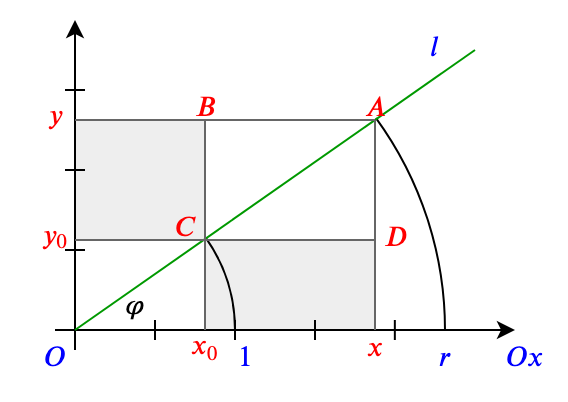
\includegraphics[scale=0.5]{linerotation.png}
\end{center}
\item Видим, что треугольники $ABC$ и $ADC$ равны по трем сторонам, также равны треугольники $Oy_0C$ и $Ox_0C$, и треугольники $OyA$ и $OxA$. Отсюда легко установить равенство площадей $x_0(y-y_0)=y_0(x-x_0)$, откуда получаем
$$
xy_0-yx_0=0.
$$
\item Поскольку $(x,y)$ --- это произвольная точка прямой $OC$ (для отрицательного $r$ все доказывается аналогично),  данное уравнение есть уравнение прямой, проходящей через начало координант с углом наклона $\ph$.
\item Отметим, что точка $(x_0,y_0)$ полностью определяется углом поворота $\ph$, т.к. является образом точки $(0,1)$ при повороте на угол $\ph$. В то же время, произвольная точка на единичной окружности однозначно задает угол поворота в интервале от 0 до $2\pi$. Таким образом, задать поворот с центром $O$ и задать точку на единичной окружности --- суть одно и то же.
\item Зная тригонометрию, можно также заметить, что $x_0=\cos\ph$ и $y_0=\sin\ph$, а отношение $y_0/x_0=\tan\ph$.
\item Кроме того, отношение $y_0/x_0$ также однозначно определяет угол поворота, но только в интервале от 0 до $\pi$.
\item Наконец, поворот прямой(!) на угол $\pi+\al$ --- это поворот на угол $\al$ с последующим отражением прямой $l$ относительно точки $O$. Но отражение прямой относительно своей же точки дает нам ту же самую прямую с тем же самым уравнением для ее точек! Таким образом, прямая, проходящая через начало координат полностью определяется тангенсом угла наклона, т.е. отношением $y_0/x_0$.
\item Но раз все дело в отношении, стало быть, прямая задается любой точкой, координаты которой находятся в таком же соотношении, что и коодинаты точки $(x_0,y_0)$, лежащие на единичной окружности. Иначе говоря, одну и ту же прямую задают также точки вида $(-x_0,-y_0)$, $(rx_0,ry_0)$, $(-rx_0,-ry_0)$, если коэффициент $r>0$. На рис. мы обозначили эти точки, соответственно, $C,A$ и $-C,-A$.
\begin{center}
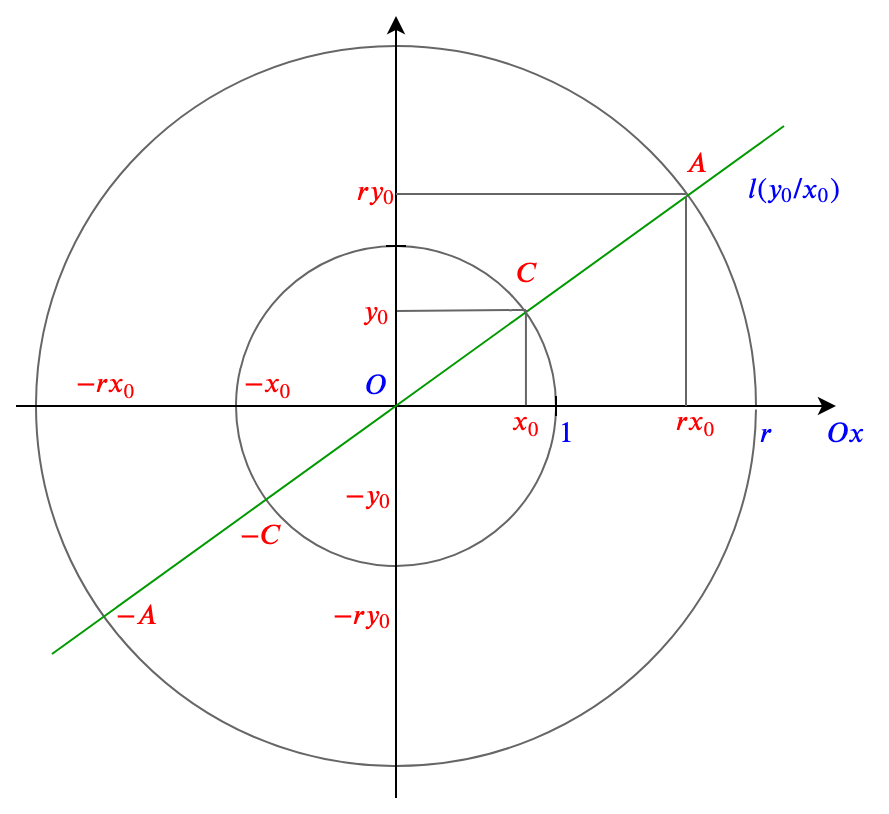
\includegraphics[scale=0.3]{line.png}
\end{center}
\item Этот вывод можно получить и более формально, просто глядя на уравнение прямой\index{Уравнение!прямой}
$$
xy_0-yx_0=0.
$$
Ведь если мы домножим обе части уравнения на $r$, ничего не изменится!
$$
x(ry_0)-y(rx_0)=0.
$$
\item Что если прямая $l$ не проходит через центр координат $O$? В этом случае мы можем сдвинуть ее на некоторый вектор так, чтобы произвольно выбранная точка этой прямой перешла в точку $O$. Обозначим эту точку на прямой $l$ за $S=(\De x,\De y)$, а сдвиг, соответственно, осуществим на вектор $(-\De x,-\De y)$.
\begin{center}
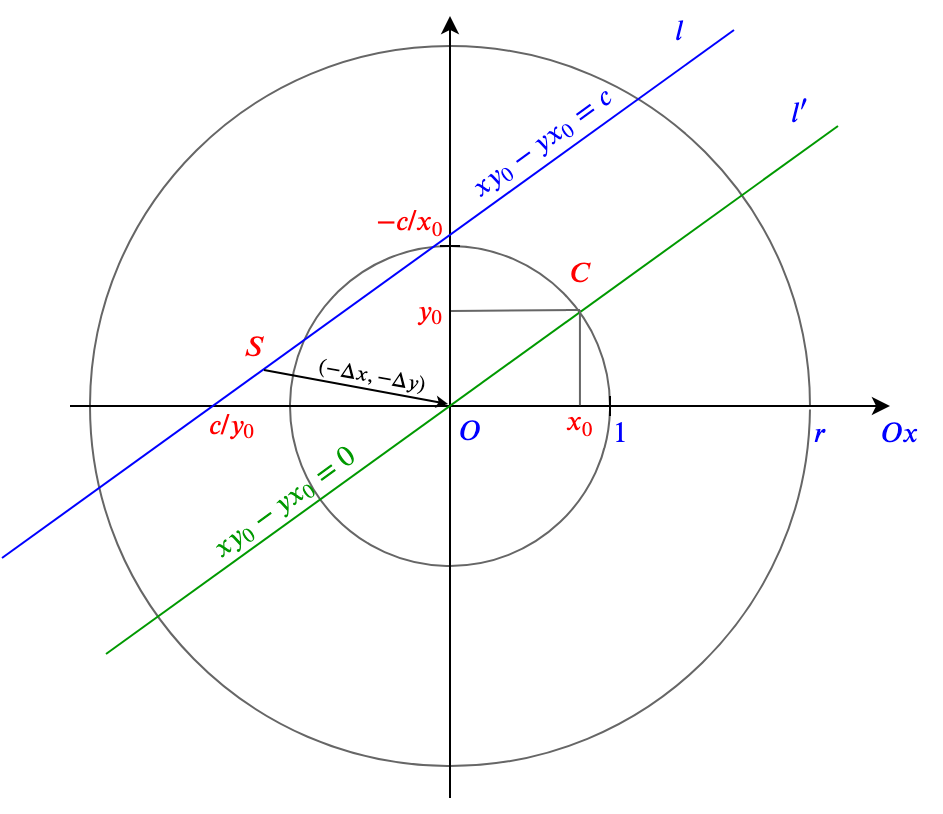
\includegraphics[scale=0.3]{lineshift.png}
\end{center}
\item Тогда смещенные координаты $(x-\De x,y-\De y)$ уже будут пробегать прямую $l'$, проходящую через центр $O$, а ее уравнение нам известно:
$$
(x-\De x)y_0 - (y-\De y)x_0=0,
$$
или
$$
xy_0-yx_0=c,\quad\mbox{где } c= y_0\De x - x_0\De y.
$$
При этом коэффициенты $(x_0,y_0)$ все так же отвечают за наклон прямой $l$ и полностью определяются тангенсом угла наклона прямой $l$ относительно положительного направления $Ox$, т.е. отношением $y_0/x_0$.
\item Может показаться, что уравнение сильно зависит от выбора точки $S$, поскольку слагаемое $c$ зависит от координат точки $S$. Покажем, что это не так. Пусть $S'=(\De x',\De y')$ --- какая-то другая точка прямой $l$. Но в этом случае она удовлетворяет найденному уравнению, т.е.
$$
\De x'y_0-\De y'x_0=c,
$$
но уравнение, найденное с помощью точки $S'$ будет иметь вид
$$
xy_0-yx_0= y_0\De x' - x_0\De y',
$$
откуда из предыдущего получаем, что вновь
$$
xy_0-yx_0=c.
$$
\item Таким образом, для нахождения $c$ мы можем выбрать любую понравившуюся нам точку прямой $l'$, например, отчку пересечения с одной из координатных осей.
\item В случае, когда $x_0\ne 0$, уравнение прямой можно переписать в виде
$$
y  = ax+b,\quad\mbox{где }a=\frac{y_0}{x_0},\; b=-\frac{c}{x_0}.
$$
В случае $x_0=0$ мы имеем вертикальную прямую $x=c$ (при угле $\ph=\pi/2$ мы получим $y_0=1$).
\end{enumerate}
\subsection*{Задачи}

\begin{enumerate}
\item В какие точки переходят точки $(0,3)$ и $(4,0)$ при повороте на $90$ градусов? На $-90$ градусов?
\item Каков угол поворота, если точка $(a,b)$ перешла в точку $(-a,-b)$? В точку $(-b,a)$? В точку $(b,-a)$?
\item Чему равен тангенс угла наклона прямой $3x-5y=7$?
\item Какой угол наклона у прямой $y=-x+3$?
\end{enumerate}


\section{Линейные уравнения в целых числах}

\lesson{Определение линейного уравнения в целях числах, однородного уравнения. Сокращение на НОД. Общее решение неоднородного уравнения.}

\begin{enumerate}
\item Поскольку мы пока владеем аппаратом только целых чисел (множество $\Z$), рассмотрим задачу о нахождении всех целых точек плоскости, через которые проходит заданная прямая. Под целыми точками плоскости мы будем понимать такие точки, координаты которых принадлежат $\Z$.
\item В общем виде \textbf{линейное уравнение в целых числах} выглядит следующим образом:\index{Линейные уравнения в целых числах}\index{Уравнение!линейное в целых числах}
$$
ax-by=c,\quad\mbox{где коэффициенты } a,b,c\in\Z.
$$
Задача: найти все такие $x,y$, тоже целые, которые удовлетворяют данному уравнению.
\item Сначала рассмотрим случай т.н. \textbf{однородного уравнения}:\index{Уравнение!линейное однородное}
$$
ax-by=0,
$$
т.е. мы отбрасываем ту часть уравнения, которая не зависит от переменных $x,y$.
\item Как мы уже знаем, данное уравнение задает прямую, проходящую через начало координат, а ее наклон определяется отношением $a/b$.
\item Для начала проверим, нельзя ли данное отношение упростить. Если числа $a,b$ имеют какой-то общий делитель, то разумно было бы на него сократить. И чтобы не проверять это много раз, сократим их сразу на $\gcd(a,b)$. Множество решений от этого не изменится, а само уравнение по-прежнему останется однородным и целочисленным:
$$
\tilde ax-\tilde by=0,\quad\mbox{где } \tilde a=\frac{a}{\gcd(a,b)},\;\tilde b=\frac{b}{\gcd(a,b)}.
$$
\item Таким образом, мы приходим к уравнению со взаимно простыми коэффициентами $\tilde a$ и $\tilde b$.
\item Перепишем уравнение иначе: $\tilde ax=\tilde by$. Заметим, что все числа здесь --- целые. Причем $\tilde by$ делится на $\tilde a$. Но так как $\tilde a$ и $\tilde b$ взаимно просты, то $y$ делится на $\tilde a$. Это есть следствие того факта, который мы доказывали ранее в разделе \ref{PrimeNumbers}: если простое число $p$ делит произведение $ab$, то оно делит $a$ или $b$ (или их обоих). Поэтому если простое $p$ делит $\tilde a$, то оно делит $\tilde by$, но оно не может делить $\tilde b$, т.к. $\gcd(p,\tilde b)=1$, значит, оно делит $y$. Это значит, что все простые, составляющие число $\tilde a$, являются делителями $y$. В то же время, эти простые не входят в $\tilde b$, поскольку $\gcd(\tilde a,\tilde b)=1$. Поэтому, если $p^\al$ входит в разложение $\tilde a$, то $p^\al$ также делит $y$. Следовательно, $y$ делится на $\tilde a$, т.е. 
$$
y=k\tilde a
$$
при некотором целом $k$.
\item Симметрично рассуждая, получаем, что $x$ делится на $\tilde b$, т.е.
$$
x=t\tilde b
$$
при некотором целом $t$.
\item Подставим эти выражения в наше однородное уравнение:
$$
\tilde a(t\tilde b)=\tilde b(k\tilde a),
$$
откуда
$$
t=k,
$$
и больше никаких ограничений на выбор коэффициента $k$ мы не имеем.
\item Таким образом, решениями уравнения $\tilde ax-\tilde by=0$ являются
$$
\begin{cases}
x  =k\tilde b=kb/\gcd(a,b), \\
y  =k\tilde a=ka/\gcd(a,b),
\end{cases}
$$
где $k\in\Z$. Эти же $x$ и $y$ являются решениями исходного однородного уравнения $ax-by=0$.
\item Вернемся к неоднородному уравнению $ax-by=c$.
\item Для начала заметим, что если данное уравнение имеет решение в целых числах, то $ax-by$ делится на $\gcd(a,b)$, а значит, $c$ делится на $\gcd(a,b)$. Поэтому, если $c$ не делится на $\gcd(a,b)$, то решений точно нет, т.е. в таком случае прямая $ax-by=c$ проходит мимо всех целых точек плоскости!
\item Покажем, что в случае делимости $c$ на $\gcd(a,b)$ решения обязательно есть, и опишем все такие решения.
\item Пусть $c=d\gcd(a,b)$.
\item В разделе \ref{PrimeNumbers} мы установили, что $\gcd(a,b)$ является линейной комбинацией чисел $a$ и $b$, т.е.
$$
\gcd(a,b) = an-bm
$$
при некоторых целых $n$ и $m$ (понятно, что знак перед $m$ можно выбирать любой, поэтому выберем так, как нам удобнее).
\item Отсюда следует, что пара чисел $(dn,dm)$ удовлетворяет уравнению $ax-by=c$, поскольку
$adn-bdm=d\gcd(a,b)=c$.
\item Итак, представив $\gcd(a,b)$ в виде линейной комбинации $a$ и $b$, мы можем найти одно решение исходного уравнения.
\item Далее применим тот же прием, что и при изучении уравнений прямых --- сдвинем прямую $ax-by=c$ так, чтобы точка $(dn,dm)$ оказалась в начале координат. Для этого введем новые переменные
$$
\hat x = x-dn,\quad \hat y = y-dm.
$$
\item Тогда получаем, что $a\hat x-b\hat y = 0$. А такое уравнение мы уже решили выше, и его решением будет пара чисел $\hat x = kb/\gcd(a,b)$ и $\hat y = ka/\gcd(a,b)$, где $k$ --- любое целое число.
\item Собирая все вместе, находим общее решение исходного уравнения:
$$
\begin{cases}
x  =kb/\gcd(a,b) + dn, \\
y  =ka/\gcd(a,b) + dm,
\end{cases}
$$
\item Таким образом, решением линейного уравнения $ax-by=c$ в целых числах является сумма общего решения однородного уравнения $ax-by=0$ и какого-нибудь частного решения исходного уравнения.

\lesson{Получение НОД с помощью алгоритма Евклида. Метод цепных дробей}

\item Основной трудностью при поиске частного решения является нахождение коэффициентов $n$ и $m$ представления $\gcd(a,b)$.
\item Это представление можно найти с помощью алгоритам Евклида. Рассмотрим для примера уравнение
$$
18x-11y=2
$$
\item Следуя алгоритму Евклида, получаем выкладки:\index{Алгоритм Евклида}
\begin{align*}
18 = & 11\cdot 1+7,\\
   & 11 = 7\cdot 1 + 4, \\
   & 7 = 4\cdot 1 + 3, \\
   & 4 = 3\cdot 1 + 1
\end{align*}
Последняя 1 --- это и есть $\gcd(18,11)$. Раскрутим алгоритм в обратную сторону:
\begin{align*}
1 & = 4-3 = 4 - (7-4) = 4\cdot 2-7 = (11-7)\cdot 2-7 =\\
  & = 11\cdot 2-7\cdot 3 = 11\cdot 2 - (18-11)\cdot 3 =\\
  & = 11\cdot 5 - 18\cdot 3.
\end{align*}
Таким образом, наши искомые числа $n=-3$, $m=-5$. Напомним, что мы ищем представление $\gcd(18,11)$ в виде $18n-11m$, исходя из чего нужно правильно выбирать знаки перед коэффициентами.

Кроме того, $d=2$, т.к. $c=2$ и $\gcd(a,b)=1$. Откуда общее решение уравнения $18x-11y=2$ получаем в виде:
$$
\begin{cases}
x  =11k - 6, \\
y  =18k - 10,
\end{cases}
$$
где $k$ --- любое целое число. Проверим:
$$
18(11k - 6) - 11(18k - 10) = 198k-198k - 108 + 110 =2.
$$
\item Наконец, приведем еще один замечательный способ найти разложение НОД. Этот метод основан на представлении дробей в виде т.н. \textbf{цепных дробей}. Пусть дано уравнение
$$
112x-34y=16.
$$
\item Ищем приближение дроби $112/34$ следующим способом:\index{Цепная дробь}
$$
\frac{112}{34} = 3 + \frac{5}{17} = 3 + \frac{1}{3+\frac{2}{5}} = 
3 + \frac{1}{3 + \frac{1}{2+1/2}}
$$
По сути дела, это --- другая запись выкладок алгоритма Евклида, поскольку мы каждый раз последовательно выделяем неполное частное предыдущих остатков.

Как только мы дошли до хвоста вида $1/k$, мы останавливаемся, отбрасываем этот хвост и сворачиваем дробь обратно, получая приближение исходной дроби:
$$
\frac{112}{34} \approx 3 + \frac{5}{17} = 3 + \frac{1}{3+\frac{2}{5}} = 
3 + \frac{1}{3 + \frac{1}{2}} = \frac{23}{7}
$$
Далее, перемножая накрест эти дроби, получаем представление для НОД:
$$
\gcd(112,34) = 112\cdot 7 - 34\cdot 23.
$$
Искомые коэффициенты: $n=7$, $m=23$. Общее решение уравнения, таким образом, получаем в виде
$$
\begin{cases}
x  = 34k +  8\cdot 7, \\
y  = 112k + 8\cdot 23 ,
\end{cases}
$$
где $k$ --- любое целое число, а $8=16/\gcd(112,34)$. Проверяем:
$$
112(34k +  8\cdot 7)-34(112k + 8\cdot 23) = 8(112\cdot 7- 34\cdot 23) = 16.
$$
\item Выше мы всюду рассматривали уравнения, в которых $x$ идет с положительным коэффициентом, а $y$ --- с отрицательным. Иначе говоря, прямая, заданная таким уравнением, имеет наклон <<вправо>>. Но уравнение может быть, например, таким
$$
5x+9y=1.
$$
Если мы хотим решать его по тем же формулам, то лучше перейти к новым переменным $\hat x=x$, $\hat y=-y$, и тогда мы получим уравнение
$$
5\hat x-9\hat y=1.
$$
Найдя его решения, мы просто меняем знак у $\hat y$, и получаем исходное уравнение.
\end{enumerate}

\subsection*{Задачи}

\begin{enumerate}
\item Найти представление $\gcd(5,9)$ с помощью алгоритма Евклида и методом цепных дробей.
\item Найти представление $\gcd(18,15)$ с помощью алгоритма Евклида и методом цепных дробей.
\item Найти представление $\gcd(225,81)$ с помощью алгоритма Евклида и методом цепных дробей.
\item Решить уравнение $5x-9y=2$ в целых числах.
\item Найти все решения уравнения $225x+81y=18$ в целях числах.
\item Найти все решения уравнения $10x-18y=3$ в целях числах или доказать, что их нет.
\end{enumerate}



\newchapter[и соизмеримость]{Рациональность}\label{Fields}

\vrezka{
В этой главе мы начинаем выход за пределы целых чисел, и прежде всего займемся построением чисел рациональных. Кроме того, мы увидим, что одними рациональными числами нельзя ограничиваться, т.к. существуют несоиземеримые с ним числа вроде корня из 2.
}


\section{Построение рациональных чисел}

\lesson{Моделирование рациональных чисел с помощью прямых с целыми коэффициентами. Прямая --- это и есть рациональное число. Умножение на целое число. Сложение прямых. Деление на целое число}

\begin{enumerate}
\item До сих пор мы часто оперировали дробями, хотя нигде их не определили. Разве что, упоминали отношение $y_0/x_0$ как некоторый параметр, определяющий угол наклона прямой на координатной плоскости в главе \ref{LinearEqs}.\index{Числа!рациональные}\index{Рациональные числа}
\item Итак, рассмотрим прямую $l$, заданную уравнением $ax-by=0$, где $a,b$ --- целые числа.
\item Для начала пусть $a=1$ и $b>1$. Легко видеть, что такая прямая проходит через точки $(0,0)$ и $(b,1)$ (см. рис.).
\begin{center}
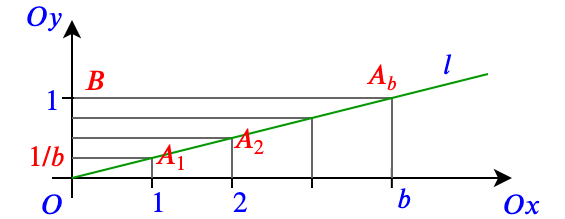
\includegraphics[scale=0.5]{section.png}
\end{center}
\item На прямой $l$ мы можем поставить точки $A_1, A_2, \dots, A_b$ в местах пересечения этой прямой с вертикальными прямыми, имеющими уравнения $x=1, x=2, \dots, x=b$, соответственно.
\item Теперь рассмотрим треугольник $OBA_b$, где точка $B=(0,1)$. В этом треугольнике мы можем провести линии, параллельные его горизонтальной стороне $BA_b$, которые отсекут на вертикальной стороне $OB$ нашего треугольника отрезки.
\item Эти отрезки будут иметь одинаковую длину по теореме Фалеса, т.к. точки на прямой $l$ также расставлены с одинаковым шагом, что следует уже из выбора вертиклаьных секущих (они идут с шагом 1).
\item Итак, на вертикальной оси мы получили $b$ одинаковых отрезков, сумма длин которых равна 1.
\item Какова же длина каждого из таких отрезков? Ответ: она равна одной $b$-ой части единицы. И эта часть записывается как дробь $1/b$. Собственно, отношение $1/b$, как мы видели ранее, является определяющим для прямой $l$.
\item Мы можем брать сумму нескольких таких частей, например, $k$ частей размера $1/b$ дают в сумме отрезок длины в $k$ раз больше, чем отрезок $1/b$. Такая часть записывается в виде дроби $k/b$.
\item Величину $k/b$ можно получить иным способом. Возьмем теперь прямую $l'$, заданную уравнением $kx+by=0$ (см. рис.).
\begin{center}
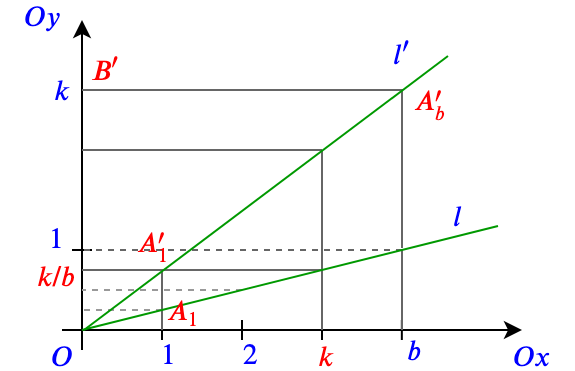
\includegraphics[scale=0.5]{sectionkb.png}
\end{center}
\item Эта прямая проходит через начало координат и точку $(b,k)$.
\item Проделаем аналогичные предыдущему построения: проведем вертикальные линии с шагом 1, а затем горизонтальные линии от точек пересечения вертикальных с прямой $l'$, и посмотрим, какие отрезки у нас получатся на оси $Oy$.
\item Нетрудно видеть, что линия, соответствующая $x=k$, для прямой $l$ отсекает на оси $Oy$ метку, которую мы обозначили как $k/b$. Но ровно ту же самую метку покажет построение с помощью вертикальной линии $x=1$ и прямой $l'$. Почему? А очень просто: достаточно сравнить уравнения этих прямых
$$
l:\;x-by=0,\quad l':\;kx-by=0.
$$
Если в первом вместо $x$ подставить $k$, а во втором вместо $x$ подставить 1, то получим одно и то же значение $y$. Отсюда и совпадение меток.
\item Таким образом, прямая $l'$ дает на оси $Oy$ шаг в $k$ раз больше, чем прямая $l$, если мы строим сечения при одном и том же $x$ (не обязательно $x=1$).
\item Получается, что прямая, заданная уравнением $kx-by=0$, задает умножение на число $k$ всех чисел, получаемых прямой, заданной уравнением $x-by=0$.
\item Рассматривая эти прямые как некие \textit{новые объекты}, мы можем ввести понятие умножения прямой на целое число. Если у нас есть прямая $\{ax-by=0\}$, то результатом ее умножения на число $k$ является прямая $\{kax-by=0\}$. Запишем это так:
$$
k\{ax-by=0\} = \{(ka)x-by=0\}.
$$
\item Заметим, что сложение (и вычитание) таких прямых определить еще проще: 
$$
\{a_1x-by=0\}\pm\{a_2x-by=0\} = \{(a_1\pm a_2)x-by=0\}.
$$
\textbf{Важно:} при сложении прямых коэффициент перед $y$ должен быть одинаковым у обеих прямых!
Только в этом случае мы получаем согласование операций сложения и умножения, а именно:
$$
\underbrace{\{ax-by=0\}+\dots+\{ax-by=0\}}_{k\mbox{ раз}} = \{kax-by=0\} = k\{ax-by=0\},
$$
\item Сложение прямых можно интерпретировать графически как сложение площадей прямоугольников с основанием $b$ и высотой $a_1$ и $a_2$. В результате получается прямоугольник с тем же основанием $b$ и высотой $a_1+a_2$. При этом прямые всегда проходят через точку $(0,0)$ и правый верхний угол прямоугольников.
\begin{center}
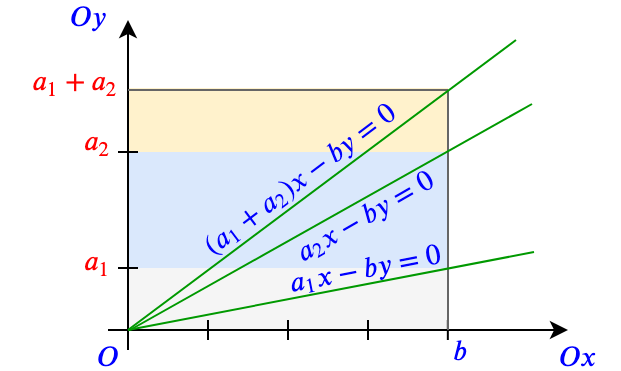
\includegraphics[scale=0.5]{linesum.png}
\end{center}
С помощью этой же картинки можно представить себе и умножение прямой на целое число $k$. Для этого нужно растиражировать соответствующий этой прямой прямоугольник вверх $k$ раз.

\item На самом же деле операции сложения, вычитания и умножения на целое число, производимые с коэффициентом перед $x$, в точности повторяют таковые операции над целыми числами (поскольку это и есть целые числа!) и, соответственно, подчиняются всем аксиомам кольца целых чисел. [А вот и более умный термин для тех, кто собирается идти в математику глубоко: \textit{прямые с общим основанием $b$ образуют векторное пространство над кольцом} $\Z$.]
\item Поэтому все прямые вида $ax-by=0$ при фиксированном $b\ne 0$ с определенныими выше операциями сложения и умножения \textit{образуют кольцо} (изоморфное кольцу целых чисел). 
\item Если вместо сложной записи $ax-by=0$, описывающей прямую, записать просто отношение $a/b$, то мы увидим, что операции с прямыми образуют в точности операции с дробями:
$$
k\frac{a}{b}  = \frac{ka}{b}\quad\mbox{и}\quad\frac{a_1}{b}+\frac{a_2}{b} = \frac{a_1+a_2}{b}.
$$
\item Заметим теперь, что уравнение $x-by=0$ прямой $l$ можно переписать иначе: $kx-(bk)y=0$. Чем оно отличается от уравнения $kx-by=0$ прямой $l'$? Очевидно, тем, что перед $y$ появился коэффициент $k$. А тепрь вспомним, что прямая $l$ задает отношение в $k$ раз меньше, чем прямая $l'$! И это значит, что если мы хотим разделить прямую $l'$ на $k$, то мы должны умножить на $k$ ее коэффициент перед $y$.
\item Итак, если мы хотим умножить прямую на число, то мы умножаем на это число коэффициент перед $x$ (прямая становится более крутой), а если мы хотим разделить прямую на число, то мы умножаем на это число коэффициент перед $y$ (прямая становится более пологой).


\lesson{Определение умножения прямых. Графическая иллюстрация умножения. Поле рациональных чисел. Почему нельзя деелить на ноль. Аксиомы поля.}


\item Делаем следующий шаг: умножение двух прямых. На самом деле, любую прямую $ax-by=0$ мы можем переписать как серию ранее определенных операций:
$$
\{ax-by=0\} = a\{x-y=0\}/b,
$$
при этом прямая $x-y=0$ имеет наклон 45 градусов и соответствует отношению 1/1, т.е. по-просту 1, и в операциях умножения может опускаться. Таким образом, умножение прямых выглядит следующим образом
\begin{gather*}
\{a_1x-b_1y=0\}\cdot\{a_2x-b_2y=0\} = \\
= a_1\{x-y=0\}/b_1\cdot a_2\{x-y=0\}/b_2 = \{a_1a_2x-b_1b_2y=0\},
\end{gather*}
а это в точности умножение дробей: $(a_1/b_1)(a_2/b_2) = (a_1a_2)/(b_1b_2)$.
\item Отсюда нетрудно получить и процедуру деления прямых друг на друга:
$$
\{a_1x-b_1y=0\}/\{a_2x-b_2y=0\} = \{(a_1b_2)x-(a_2b_1)y=0\},
$$
что соответствует операции с дробями:
$$
\frac{a_1}{b_1}/\frac{a_2}{b_2} = \frac{a_1b_2}{a_2b_1}.
$$
\item Наконец, чтобы научиться складывать произвольные прямые, мы должны уметь сводить сложение произвольных прямых к сложению прямых с одинаковым коэффициентом перед $y$, т.к. сложение мы определили выше только для данного случая.
\item Но и это не проблема:
\begin{gather*}
(a_1x-b_1y=0)+(a_2x-b_2y=0) = (a_1b_2x-b_1b_2y=0) + (a_2b_1x-b_1b_2y=0) = \\
= ((a_1b_2+a_2b_1)x-(b_1b_2)y=0),
\end{gather*}
что соответствует операциям с дробями
$$
\frac{a_1}{b_2}+\frac{a_2}{b_2} = \frac{a_1b_2+a_2b_1}{b_1b_2}.
$$
\item Следующая картинка показывает <<арифметику прямых>> с произвольными параметрами.
\begin{center}
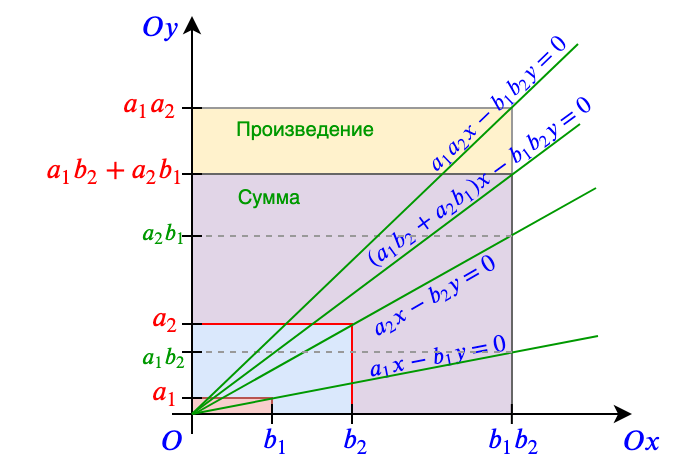
\includegraphics[scale=0.5]{linear.png}
\end{center}
Здесь маленькие прямоугольники соответствуют исходным прямым с уравнениями $a_1x-b_1y=0$ и $a_2x-b_2y=0$, пунктиром отмечены приведенные к общему основанию $b_1b_2$ прямоугольники, большой темный прямоугольник соответствует их сумме (буквально однин приставлен сверху к другому), большой светлый прямоугольник --- произведению (помножены основания и помножены высоты). Рисунок не учитывает масштаб!

\item В целом картина представления рациональных чисел с помощью прямых с целочисленными коэффициентами выглядит следующим образом:\index{Рациональные числа}\index{Числа!рациональные}
\begin{center}
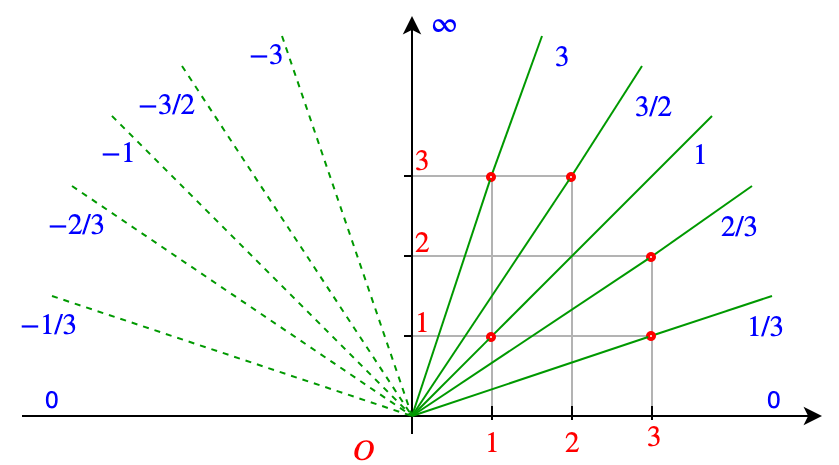
\includegraphics[scale=0.4]{ratio.png}
\end{center}

\item Итак, имея только множество целых чисел $\Z$, мы построили на плоскости всевозможные прямые, заданные линейными уравнениями с целыми коэффициентами, научились их складывать, вычитать, умножать и делить. Тем самым, мы построили новую алгебраическую структуру, которая называется \textbf{полем}. Поле --- это кольцо, в котором можно делить на любое число, кроме нуля.\index{Поле}
\item Записывая эти прямые не уравнениями, а отношением коэффициентов (вместо $ax-by=0$ пишем $a/b$), мы получаем \textbf{поле рациональных чисел}, которое принято обозначать $\Q$.
\item На самом деле, в нашем построении есть еще и такая прямая, которая соответствует бесконечности. Это прямая, заданная уравнением $x=0$. А нулевая прямая определяется уравнением $y=0$. В полном соответствии с установленными правилами, мы можем заметить, что если $a\ne 0 \ne b$, то
\begin{gather*}
\{ax-by=0\}\{y=0\}=\{y=0\},\;\{ax-by=0\}\{x=0\}=\{x=0\},\\ 
\{ax-by=0\}/\{y=0\}=\{x=0\},\;\{ax-by=0\}/\{x=0\}=\{y=0\},
\end{gather*}
или, иначе:
$$
\frac{a}{b}\cdot 0 = 0,\quad\frac{a}{b}\cdot\infty = \infty,\quad
\frac{a}{b}/ 0 = \infty,\quad\frac{a}{b}/\infty = 0
$$
при $a\ne 0\ne b$,
т.е. деление на ноль дает бесконечность, а деление на бесконечность дает ноль.
\item Но тут кроется проблема: $\{x=0\}\cdot\{y=0\}=\{0x-0y=0\}$ --- такое уравнение на задает прямую, его решением является вся плоскость! Проще говоря, при умножении $0\cdot\infty$ может получиться любое число!
\item Поэтому при определении поля бесконечный элемент не постулируется и, соответственно, деление на ноль не разрешено.
\item Приведем полный формальный список аксиом поля. Множество $F$ с операциями $+$ и $\cdot$ называется \textbf{полем}, если:\index{Поле!аксиомы поля}
\begin{enumerate}[{\bf Field}1]
\item $a,b\in F\Rightarrow a+b\in F, a\cdot b\in F$ (замкнутость операций);
\item $a,b,c\in F\Rightarrow (a+b)+c=a+(b+c), (a\cdot b)\cdot c = a\cdot (b\cdot c)$ (ассоциативность операций);
\item для всех $a,b\in F$ имеем $a+b=b+a$ и $a\cdot b=b\cdot a$ (коммутативность операций);
\item существует элемент $0\in F$ такой, что $a+0=0+a=a$ для всех $a\in F$ (аксиома нуля);
\item для всякого элемента $a\in F$ существует противоположный $-a$ такой, что $a+(-a)=0$ (аксиома противоположного элемента);
\item существует элемент $1\in F$ такой, что $a\cdot 1=1\cdot a=a$ для всех $a\in F$ (аксиома единицы),
\item для всякого элемента $a\in F$, если $a\ne 0$, то существует обратный $a^{-1}$ такой, что $a\cdot a^{-1}=1$ (аксиома обратного элемента).
\item для всех $a,b,c\in F$ имеем $(a+b)\cdot c=(a\cdot c)+(b\cdot c)$, $c\cdot(a+b)=(c\cdot a)+(c\cdot b)$ (правая и левая дистрибутивность);
\end{enumerate}
\item Иначе говоря, поле --- это \textit{коммутативное кольцо с единицей, в котором каждый ненулевой элемент обратим}. На следующей схеме представлено формирование таких понятий как поле и кольцо из более простых свойств (или аксиом):
\begin{center}
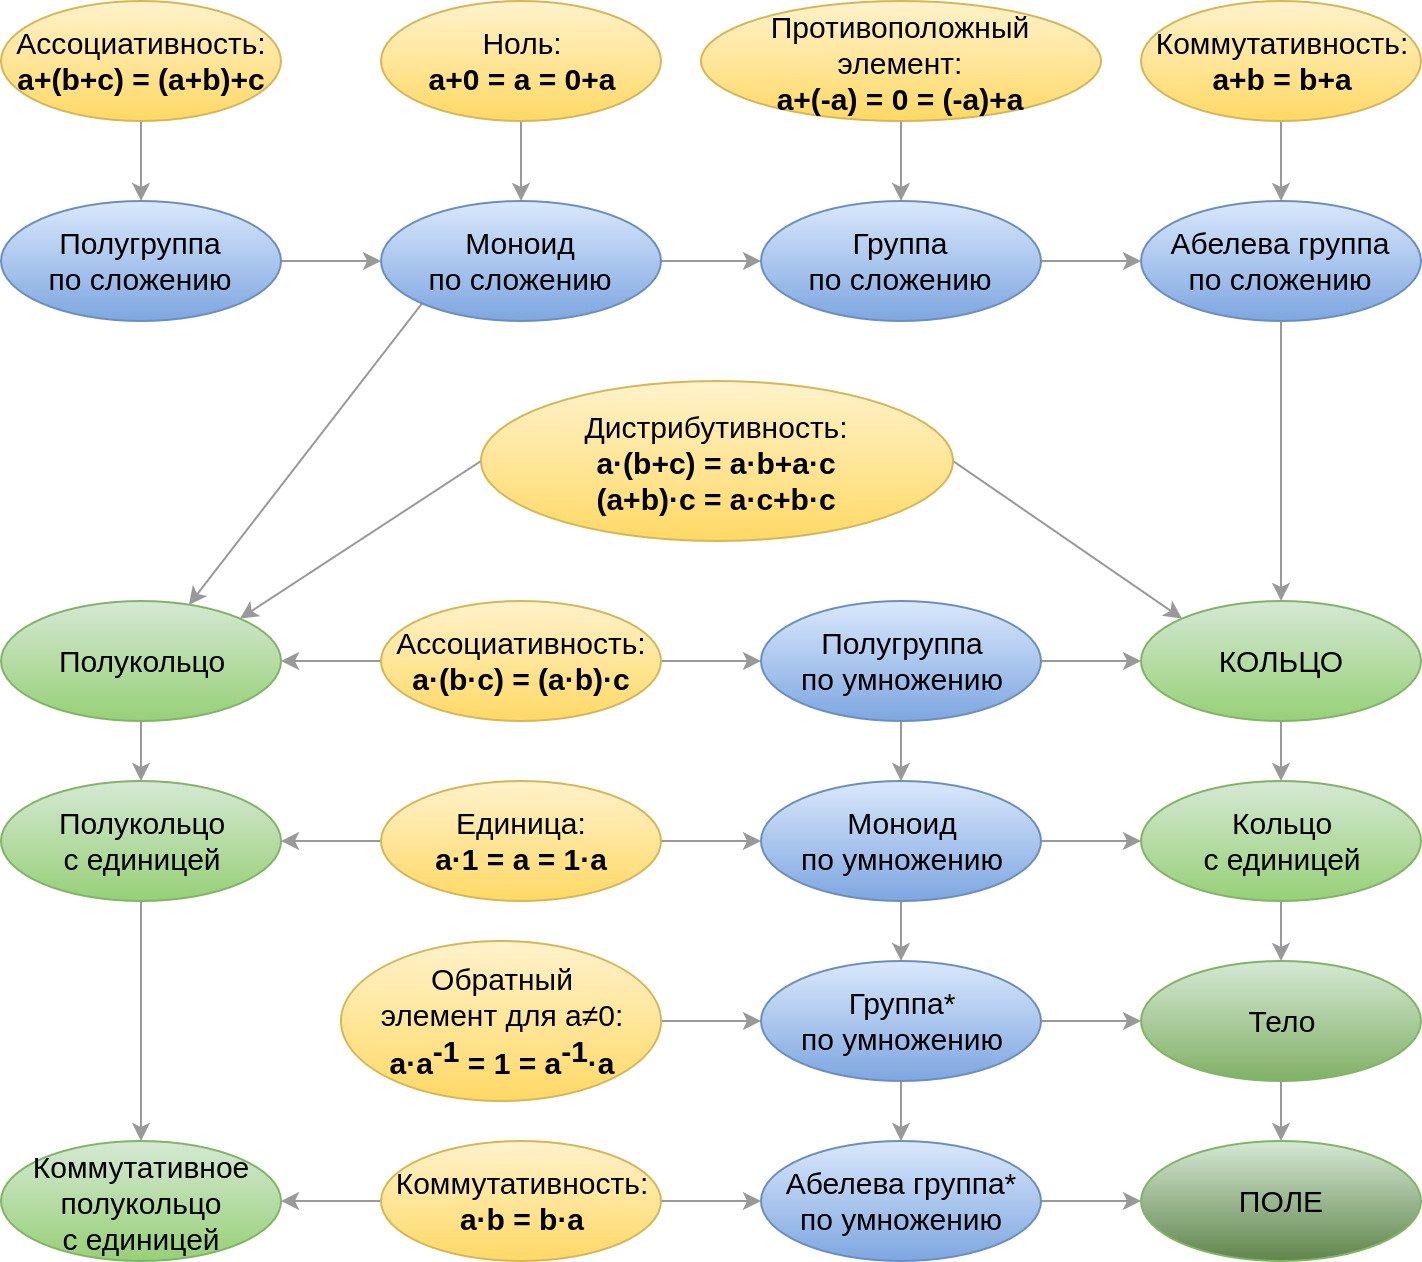
\includegraphics[scale=0.25]{Ring.png}
\end{center}
\end{enumerate}




\section{Соизмеримость. Иррациональности}

\lesson{Рциональные числа как расширение кольца целых чисел. Они определяются линейными уравнениями в целых числах. Разбор уравнения $x^2-2=0$. Доказательство иррациональности $\sqrt 2$ через ОТА, цепные дроби и графически. Несоизмеримость $\sqrt 2$ и 1. Рациональное $\Leftrightarrow$ конечная цепная дробь}

\begin{enumerate}
\item Рациональные числа мы построили с помощью прямых, заданных уравнением $ax-by=0$, где $a$ и $b$ --- произвольные целые числа, одновременно не равные нулю. Оказалось, что такая прямая отсекает отрезки длины $a/b$ на вертикальной оси, когда $x$ меняется с шагом 1, т.е. пробегает все целые числа. В частности, при $x=1$ мы получаем уравнение $by=a$, решением которого является единственное число $y=a/b$.
\item Говоря алгебраическим языком, рациональные числа --- это корни линейных уравнений, т.е. уравнений вида $a-by=0$, с целыми коэффициентами $a,b$.
\item Таким образом, выход в поле рациональных чисел происходит при попытке разрешить линейное уравнение, заданное над кольцом целых чисел.
\item Что если мы рассмотрим линейное уравнение, но над полем рациональных чичел? Будет ли оно разрешимо?
\item Пусть $rx-q=0$ и $r,q\in\Q$. Тогда представим эти рациональные числа в виде дробей $r=a/b$, $q=c/d$, откуда
$$
0=rx-q = \frac{a}{b}x-\frac{c}{d} = \frac{adx-cb}{bd},
$$
откуда ясно, что данное уравнение эквивалентно линенойму уравнению $(ad)x-(cb)=0$ с целыми коэффициентами, а значит, разрешимо в поле рациональных чисел.
\item Таким образом, поле $\Q$ замкнуто относительно линейных уравнений. Посмотрим, как оно справится с уравнениями более высокой степени! Рассмотрим уравнение $x^2-2=0$. Это уравнение с целыми коэффициентами (1 и 2). Разрешимо ли оно в $\Z$ или хотя бы в $\Q$?
\item Ответ: нет! Предположим, что $x=n/m$ разрешает такое уравнение, т.е. $(n/m)^2=2$. Предположим сразу же, что $n\perp m$, т.е. дробь $n/m$ несократимая. Далее имеем
$$
n^2=2m^2.
$$
Отсюда видно, что $n^2$ делится на 2, а значит, $2$ входит в разложение числа $n^2$ по степеням простых. Проблема в том, что если бы 2 не входила в разложение числа $n$, то ее не было бы и в разложении числа $n^2$, т.к. $n^2$ есть поризведение степеней тех же самых простых, что и $n$, только в удвоенной степени. А значит, $n$ делится на 2, откуда следует, что $n^2$ делится на 4. Но тогда $m^2$ делится на 2 и, аналогично рассуждая, получаем, что и $m$ делится на 2. А это уже противоречит тому, что дробь $n/m$ несократимая --- ее как минимум можно сократить на 2.

Следовательно, корень уравнения $x^2-2=0$ не может быть рационалным числом.
\item Тем не менее, положительный корень такого уравнения можно оценивать сверху и снизу сколь угодно точно. Например, корень извлекается из числа 2.25 и равен 1.5, при этом $x^2=2<2.25$, так что $x<1.5$. В то же время, $2>1.96=1.4^2$, так что $x>1.4$. Можно еще усилить оценку: $1.41<x<1.42$. И так далее. Это позволяет нам думать, что на самом деле число такое есть, просто оно сидит где-то между рациональными числами. Обоснование его существования мы отложим на потом, а пока просто обозначим его $\sqrt 2$.
\item Есть ее один способ удостовериться в том, что $\sqrt 2$ не является рациональным числом. И тут снова нам на выручку приходят цепные дроби. Теперь-то мы вправе ими оперировать!
\item Воспроизведем алгоритм Евклида для дроби $\al = r_0/r_1$, считая, что $r_0>r_1$ (если это не так, то приведем дробь к виду $1/(r_1/r_0)$ и будем работать дальше только со знаменателем). Как и раньше, будем выделять остаток $r_{k+1}$ от деления $r{k-1}$ на $r_k$ и сохранять неполное частное $m_k$. Только запишем весь алгоритм не в несколько строк, а в виде многоэтажной дроби. Поехали!\index{Цепная дробь}
\begin{multline*}
\frac{r_0}{r_1} = \frac{k_1r_1+r_2}{r_1} = \boxed{k_1}+\frac{1}{\frac{r_1}{r_2}} =
\boxed{k_1} + \frac{1}{\frac{k_2r_2+r_3}{r_2}} =  \\
= \boxed{k_1} + \frac{1}{\boxed{k_2} + \frac{1}{r_3/r_2}} = 
\boxed{k_1} + \frac{1}{\boxed{k_2} + \frac{1}{\boxed{k_3} + \ddots \frac{1}{\boxed{k_n}+r_{n+1}/r_n}}},
\end{multline*}
где $r_0>r_1>r_2>\dots>r_n>r_{n-1}$.

\item Поскольку остатки всегда являются натуральными числами, рано или поздно этот алгоритм прервется. Пусть это случится на шаге с номером $n$, так что мы полагаем $r_{n+1}=0$, и цепная дробь закончится на числе $k_n$.
\item В таком случае цепную дорбь принято записывать последовательностью выделенных на каждом шаге целых частей:
$$
\frac{r_0}{r_1} = [k_1,k_2,\dots,k_n].
$$
\item Отсюда следует, что всякая рациональная дробь представима в виде конечной цепной дроби. Обратное, очевидно, также верно, ибо каждую конечную цепную дробь можно свернуть по правилам арифметики в обычную рациональную дробь.
\item Заметим также, что любое целое число представлятся в виде тривиальной цепной дроби, в которой есть только $k_1$.
\item Алгоритм Евклида можно применять к любым числам, лишь бы можно было выделять остаток от деления. Например, его можно применить к паре чисел $\pi/2$ и $\pi/3$ и получить конечную цепную дробь. А все потому, что отношение этих чисел является рациональным числом $3/2$. Поэтому, если отношение двух чисел $a/b$ рационально, их принято называть \textbf{соизмеримыми}.\index{Числа!соизмеримые}
\item\label{soizm} Соизмеримые числа хорошо иллюстрируются следующей картинкой:
\begin{center}
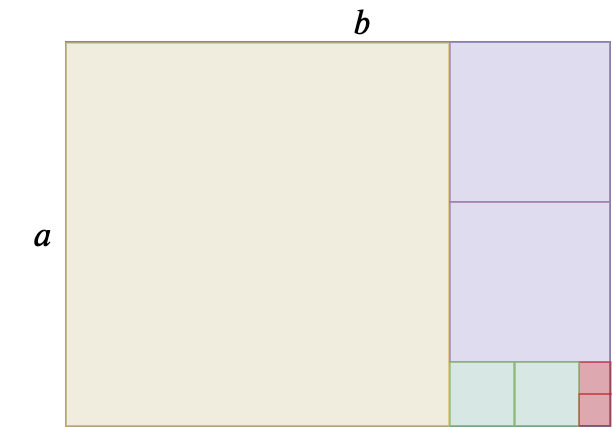
\includegraphics[scale=0.3]{soizmer.png}
\end{center}
Видим, что прямоугольник $a\times b$ мы делим на квадраты, каждый раз выбирая максимальный квадрат, который вписывается в оставшуюся область. Если $a$ и $b$ соизмеримы, то порцесс разрзания прямоугольника на квадраты закончится за конечное число шагов, причем количество одинаковых квадратов, посчитанное в порядке их убывания, есть как раз те самые числа $k_1,k_2,\dots,k_n$, появляющиеся в записи цепной дроби. Поскольку вырезание макисмального квадрата --- это не что иное как процесс выделения целой части из остатка, т.е. алгоритм Евклида.
\item То, что сами числа $a$ и $b$ при этом могт не быть целыми или рациональными --- не важно. Важно, что их отношение рационально. Также легко видеть, что всякое рациональное число соизмеримо с 1 и, наоборот, всякое число, соизмеримое с 1, рационально.
\item Посмотрим теперь, что происходит при попытке записать цепную дробь для $\sqrt 2$.
\item Мы уже знаем, что $1<\sqrt 2<2$, кроме того, $(\sqrt 2+1)=1/(\sqrt 2-1)$ так что
\begin{multline*}
\sqrt 2 = \boxed{1} + (\sqrt 2-1) = \boxed{1} + \frac{1}{1/(\sqrt 2-1)} = 
\boxed{1} + \frac{1}{\sqrt 2+1} = \\ 
= \boxed{1} + \frac{1}{\boxed{2} + (\sqrt 2-1)} = 
\boxed{1} + \frac{1}{\boxed{2} + \frac{1}{\sqrt 2+1}} = 
\boxed{1} + \frac{1}{\boxed{2} + \frac{1}{\boxed{2} + \frac{1}{\boxed{2} + \dots}}}
\end{multline*}
\item Как видим, остатком после выделения целой части всегда является одно и то же число $\sqrt 2-1$, и процесс алгоритма Евклида никогда не остановится. При этом цепная дробь характеризуется последовательностью одинаковых целых частей, равных 2. То есть представление для корня из 2 в виде цепной дроби будет бесконечным:
$$
\sqrt 2 = [1,2,2,2,2,2,\dots],
$$
и, следовательно, $\sqrt 2$ не является рациональным числом.
\item Геометричексий алгоритм Евклида здесь тоже зацикливается. Действительно, возьмем прямоугольник со сторонами $1+\sqrt 2$ и 1. Следуя алгоритму, вырежем из него два квадрата $1\times 1$. Посмотрим, какой прямоугольник остался: его сторонами будут $1$ и $\sqrt 2-1$. А в каком соотношении друг к другу они находятся?
$$
\frac{1}{\sqrt 2-1}=\frac{\sqrt{2}+1}{(\sqrt 2-1)(\sqrt 2+1)}=\sqrt 2+1.
$$
Таким образом, перед нами уменьшенная копия исходного прямоугольника. И если мы продолжим вырезать квдараты, будем вновь и вновь получать один и тот же прямоугольник, только всё меньшего размера.


\lesson{Иррациональное число. Поле $\Q[\sqrt 2]$. Дальнейшие расширения? Есть ли поле, не требущее расширения?}



\item Числа, не яляющиеся рациональными, называются \textbf{иррациональными}.\index{Числа!иррациональные}
\item Наличие иррационального числа $\sqrt 2$ позволяет нам рассмотреть числа вида $r+q\sqrt 2$, где $r,q\in\Q$.
\item Множество таких чисел, полученных присоединением к полю $\Q$ положительного корня уравнения $x^2=2$, принято обозначать $\Q[\sqrt 2]$ и называть расширением поля $\Q$.
\item Очевидно, что множество $\Q[\sqrt 2]$ замкнуто относительно сложения и вычитания, т.к.
$$
(r_1+q_1\sqrt 2)+(r_2+q_2\sqrt 2)=(r_1+r_2)+(q_1+q_2)\sqrt 2,
$$
т.е. числом такого же вида.
\item Чуть сложнее увидеть, что и умножение и деление таких чисел имеют тоже вид $r+q\sqrt 2$:
$$
(r_1+q_1\sqrt 2)(r_2+q_2\sqrt 2)=(r_1r_2+2q_1q_2)+(r_1q_2+r_2q_1)\sqrt 2,
$$
\begin{multline*}
\frac{r_1+q_1\sqrt 2}{r_2+q_2\sqrt 2}=\frac{(r_1+q_1\sqrt 2)(r_2-q_2\sqrt 2)}{(r_2+q_2\sqrt 2)(r_2-q_2\sqrt 2)}=
\frac{(r_1r_2-2q_1q_2)+(r_2q_1-r_1q_2)\sqrt 2}{r_2^2-2q_2^2}= \\
=\frac{r_1r_2-2q_1q_2}{r_2^2-2q_2^2}+\frac{r_2q_1-r_1q_2}{r_2^2-2q_2^2}\sqrt 2,
\end{multline*}
т.е. в обоих случаях результат снова находится в $\Q[\sqrt 2]$.
\item Это значит, что множество $\Q[\sqrt 2]$ с обычными операциями сложения и умножения является полем.
\item В поле $\Q[\sqrt 2]$ уравнение $x^2-2=0$ разрешимо. Причем, в нем лежат оба корня данного уравнения: $\sqrt 2$ и $-\sqrt 2$.
\item Отметим еще один важный факт. В поле $\Q[\sqrt 2]$ выражение $x^2-2$ можно записать в виде произведения линейных членов $(x-\sqrt 2)(x+\sqrt 2)$, поскольку $\sqrt 2$ здесь стал разрешенным числом. Точно так же мы ранее сначала не могли записывать уравнения $0.5x-1=0$, т.к. работали только с целыми числами (но могли заменить его эквивалентным уравнением $x-2=0$), а после выхода в поле $\Q$ у нас появилась возможность использовать дробные коэффициенты.
\item Возникает резонный вопрос: а если уравнение какое-то более сложное? Например, $x^5+3x^3-5=0$. Всегда ли его можно разложить на линейные множители в поле $\Q[\sqrt 2]$? Или понадобится какое-то новое расширение $\Q$?
Иначе говоря, всегда ли будут корни такого уравнения лежать в построенных нами полях?
\item Ответ: нет. Но существует такое всеобъемлющее поле, в котором это действительно возможно. И постепенно мы дойдем до него...
\end{enumerate}


\subsection*{Задачи}

\begin{enumerate}
\item Разложите в цепную дробь числа $9/5$, $22/7$, $3/13$, $55/27$.
\item Какое число и цепная дробь щашифрованы на картинке в пункте \ref{soizm}?
\item Найти цепную дробь для $\sqrt 3$.
\item Найти цепную дробь для отношения 
$$
\frac{\sqrt 2+1}{\sqrt 2-1}.
$$
Соизмеримы ли эти числа?
\end{enumerate}




\newchapter{Исчисление остатков}\label{ostatki}

\vrezka{
Арифметика остатков дает богатый фактологичекий материал для изучения свойств простых чисел, а также позволяет по-новому взглянуть на операции Минковского с числовыи множествами и выйти на такие важные вехи теории множеств, как виды отношений и фактормножества.
}

\section{Арифметика остатков}

\lesson{Сюжет с минутами и часами. Исчисление дней недели. Високосные годы. Определение сравнимости чисел по модулю.}

\begin{enumerate}
\item Рассмотрим бытовую задачу. Вам нужно выключить печку через 40 минут, но у вас нет таймера, зато есть будильник, на котором можно выставить время звонка. Сейчас 12:30, на какое время требуется поставить будильник? Ответ: 13:10. Почему так? Дело в том, что в часе 60 минут, и если к 30 минутам прибавить 40, получается 70 минут, что больше часа. Поэотму добавляем 1 час и остаток --- 10 минут.
\item Еще пример: сколько часов будет через 20 часов, если сейчас 8 утра? Можно решать аналогично: $8+20=28$, затем убираем полные сутки, т.е. 24 часа, остается 4 часа утра.
\item Можно решать иначе. 20 часов --- это $-4$ часа от суток. Следовательно, нужно просто вычесть из 8 утра 4 часа и получим те же 4 часа утра.
\item Во всех случаях мы решаем задачу нахождения остатка от деления на некоторое число. В случае минут это 60, в случае часов это 24.
\item Когда вас просят отметить в анкете количество полных лет, то вам по сути нужно найти неполное частное от деления вашего возраста на 1 год. Конечно, в данном случае нам это просто сделать, т.к. каждый год мы запоминаем именно количество прожитых лет, а не дней или недель.
\item Но, например, во многих сферах деятельности планирование календаря происходит неделями (и даже у себя в компьютере в настройках календаря вы можете вывести номер текущей недели в году). А сколько недель в году? Для этого нужно найти неполное частное от деления 365 (или 366) на 7, оно составляет 52.
\item Остаток от деления на неделю есть число от 0 до 6, которое определяет сдвиг вперед относительно текущего дня недели. Например, если сегодня четверг, то какой день недели будет через 30 дней? Мы выбрасываем из 30 4 полных недели, что составляет 28 дней, и находим остаток, который равен 2. Это значит, что через 30 дней будет четверг плюс 2 дня, т.е. суббота.
\item Точно так же можно легко заметить, что каждый год происходит смещение дат на 1 или два дня вперед относительно дней недели. Так, если в этом году 1 января было средой, то в следующем оно будет или четвергом (если мы не переходим через 29 февраля), или пятницей (если текущий год --- високосный, т.е. содержит 366 дней), как на картинке ниже.

\begin{center}
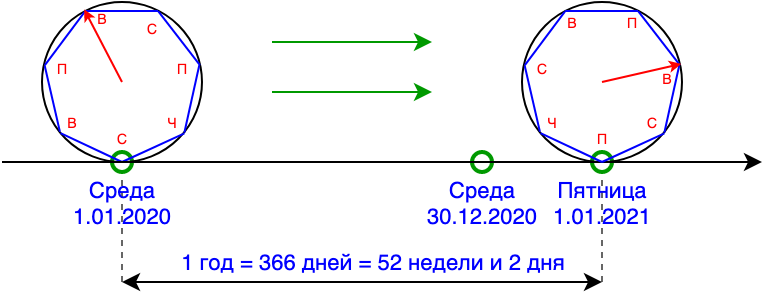
\includegraphics[scale=0.4]{weekdays.png}
\end{center}

\item Каждые 28 лет (а 28 --- это наименьшее общее кратное 7 и 4) соответствие дат и дней недели повторяется.
\item При расчетах на более длительные периоды, а именно, при переходе через 1900 год или 2100 год, нужно учитывать также, что 3 раза за 400 лет не происходит добавление лишнего дня (29 февраля) для более точного соответствия календаря астрономическому году, т.е. 1900, 1800, 1700 годы не являются високосными, как и 2100, 2200 и 2300.
\item Тем не менее, часто в жизни встречается задача вычисления дня недели, и здесь нам на помощь приходит исчисление остатков по модулю 7. Например, сегодня 21 марта 2020 суббота, а нам нужно знать, какой день недели будет 31 августа 2020. Сначала мы находим день недели 21 августа, т.к. до этой даты целое число месяцев. При этом мы 3 раза переходим через 31 число (март, май, июль) и 2 раза --- не переходим (апрель, июнь). Следовательно, 3 раза прибавляется остаток 3, и 2 раза --- остаток 2, итого сумма остатков составляет 13. Но это больше 7, причем очень близко к 14, поэтому сумму остатков мы запишем как -1. Наконец, остается добавить 10 дней (от 21 августа до 31 августа). Итого получается 9, а по модулю 7 --- всего 2. Таким образом, 31 августа 2020 года есть понедельник!
\item Из приведенной выше картинки с семиугольником на окружности, совмещенной с прямой линией, мы можем ясно представить себе, как работает исчисление остатков по модулю 7, т.е. исчисление дней недели. Мы катим окружность по прямой времени, пока не достигнем нужной нам даты. При этом неважно, сколько целых оборотов совершит семиугольник, т.е. сколько недель мы проедем, а вот последний полувиток как раз и дает нам ответ на вопрос о дне недели. Так что, если мы пронумеруем дни недели цифрами от 0 до 6, то любое расстояние между датами можно представить как какое-то целое количество недель плюс остаток, лежащие в диапазоне от 0 до 6 (включительно).
\item Эта картинка легко обобщается на случай произвольного основания. Представим, что в неделе у нас не 7 дней, а, например, 28 (лунный месяц), и тогда любое расстояние между датами выражается как целое число 28-дневных циклов плюс некоторый остаток от 0 до 27. И так далее.
\item Таким образом, мы приходим к тому, что всякое натуральное число (количество) можно представить в виде $a=km+b$, где $k$ --- неполное частное от деления $a$ на $m$, $b$ --- остаток от деления, который находится в промежутке от 0 (включая) до $m$ (не включая).
\item Равенство $a=km+b$ при исчислении остатков принято записывать так:
$$
a\equiv b\pmod m,
$$
Читается: $a$ \textbf{сравнимо с} $b$ (по модулю $m$).\index{Отношение!сравнимости по модулю}\index{Сравнение по модулю}

Причем, если модуль $m$ известен из контекста и не меняется при вычислениях, то его можно опускать, записывая просто $a\equiv b$. 

\item На картинке, приведенной выше, даты 1 января 2020 и 30 декабря 2020 сравнимы по модулю 7, т.е. по дням недели.
А про интервал в 366 дней мы запишем $366\equiv 2\pmod 7$. Такая запись никак не информирует нас о коэффициенте $k$ (количестве целых недель), но показывает самое главное --- сколько дней надо прибавить к среде.


\lesson{Таблицы сложения и умножения для разных модулей. Анализ нулевых строк и теорема об остатках. Сравниваем $\Z_5^*$ и $\Z_8^*$}

\item Остатками можно оперировать так же, как обычными числами, сбрасывая всякий раз накопленные при сложении целые <<оброты>> модулей. Иначе говоря, если мы хотим, например, к текущей среде прибавить 6 дней, то мы совмещаем наш семиугольник вершиной <<среда>> с прямой времени, а затем прокатываем его вперед на 6 делений (что чуть меньше полного оборота), и в точке касания с прямой получаем вторник. Заметим, что ровно тот же результат мы получим, если прокатим семиугольник назад на 1 деление. Это значит, что числа 6 и -1 сравнимы по модулю 7. И на практике можно также пользоваться отрицательными числами для исчисления остатков.
\item Ранее мы много времени уделяли таблицам композиций движений многоугольников. И, как мы помним, композиция вращений многоугольника соответствовала сложению углов этих вращений. При этом мы также отбрасывали 360 градусов (или $2\pi$), если сумма углов переваливала за полный оборот. При описании конечных подгрупп движений правильных многоугольников мы выяснили, что каждый поворот является степенью некоторого минимального поворота на угол $2\pi/n$ (для $n$-угольника), т.е. все повороты выражаются углами $k(2\pi/n)$, где $k=0,\dots,n-1$ (ничего не напоминает?).
\item Забудем теперь про вращения и углы, а просто понаблюдаем за степенями этих поворотов при композициях, т.е. при сложении углов. Для примера рассмотрим случаи $n=7$ и $n=8$, и выпишем таблицу композиций, которая представлят собой таблицу сложения остатков по модулям 7 и 8, соответственно.
\item Таблицы сложения остатков по модулям 7 и 8:\index{Таблица сложения по модулю}
\begin{center}
\begin{tabular}{c||c|c|c|c|c|c|c|}
  & 0 & 1 & 2 & 3 & 4 & 5 & 6 \\ \hline\hline
0 & 0 & 1 & 2 & 3 & 4 & 5 & 6 \\ \hline
1 & 1 & 2 & 3 & 4 & 5 & 6 & 0 \\ \hline
2 & 2 & 3 & 4 & 5 & 6 & 0 & 1 \\ \hline
3 & 3 & 4 & 5 & 6 & 0 & 1 & 2 \\ \hline
4 & 4 & 5 & 6 & 0 & 1 & 2 & 3 \\ \hline
5 & 5 & 6 & 0 & 1 & 2 & 3 & 4 \\ \hline
6 & 6 & 0 & 1 & 2 & 3 & 4 & 5 \\ \hline
\end{tabular}
\quad
\begin{tabular}{c||c|c|c|c|c|c|c|c|}
  & 0 & 1 & 2 & 3 & 4 & 5 & 6 & 7 \\ \hline\hline
0 & 0 & 1 & 2 & 3 & 4 & 5 & 6 & 7 \\ \hline
1 & 1 & 2 & 3 & 4 & 5 & 6 & 7 & 0 \\ \hline
2 & 2 & 3 & 4 & 5 & 6 & 7 & 0 & 1 \\ \hline
3 & 3 & 4 & 5 & 6 & 7 & 0 & 1 & 2 \\ \hline
4 & 4 & 5 & 6 & 7 & 0 & 1 & 2 & 3 \\ \hline
5 & 5 & 6 & 7 & 0 & 1 & 2 & 3 & 4 \\ \hline
6 & 6 & 7 & 0 & 1 & 2 & 3 & 4 & 5 \\ \hline
7 & 7 & 0 & 1 & 2 & 3 & 4 & 5 & 6 \\ \hline
\end{tabular}
\end{center}
Таблица сложения получается последовательными циклическими сдвигами верхней строки влево.


\item Помимо сложени остатков мы можем их умножать (в терминологии вращений многоугольника умножение соответствует многократной композиции одинаковых поворотов, так что первое число произведения отвечает за величину поворота, а второе --- за его кратность, либо наоборот).  Таблица умножения остатков по модулям 7 и 8 (отметим важную особенность этих таблиц: они имеют центральную симметрию, если вычеркнуть нулевые строку и столбец):\index{Таблица умножения по модулю}
\begin{center}
\begin{tabular}{c||c||c|c|c|c|c|c|}
  & 0 & 1 & 2 & 3 & 4 & 5 & 6 \\ \hline\hline
0 & 0 & 0 & 0 & 0 & 0 & 0 & 0 \\ \hline\hline
1 & 0 & 1 & 2 & 3 & 4 & 5 & 6 \\ \hline
2 & 0 & 2 & 4 & 6 & 1 & 3 & 5 \\ \hline
3 & 0 & 3 & 6 & 2 & 5 & 1 & 4 \\ \hline
4 & 0 & 4 & 1 & 5 & 2 & 6 & 3 \\ \hline
5 & 0 & 5 & 3 & 1 & 6 & 4 & 2 \\ \hline
6 & 0 & 6 & 5 & 4 & 3 & 2 & 1 \\ \hline
\end{tabular}
\qquad
\begin{tabular}{c||c||c|c|c|c|c|c|c|}
  & 0 & 1 & 2 & 3 & 4 & 5 & 6 & 7 \\ \hline\hline
0 & 0 & 0 & 0 & 0 & 0 & 0 & 0 & 0 \\ \hline\hline
1 & 0 & 1 & 2 & 3 & 4 & 5 & 6 & 7 \\ \hline
2 & 0 & 2 & 4 & 6 & 0 & 2 & 4 & 6 \\ \hline
3 & 0 & 3 & 6 & 1 & 4 & 7 & 2 & 5 \\ \hline
4 & 0 & 4 & 0 & 4 & 0 & 4 & 0 & 4 \\ \hline
5 & 0 & 5 & 2 & 7 & 4 & 1 & 6 & 3 \\ \hline
6 & 0 & 6 & 4 & 2 & 0 & 6 & 4 & 2 \\ \hline
7 & 0 & 7 & 6 & 5 & 4 & 3 & 2 & 1 \\ \hline
\end{tabular}
\end{center}
\item Отметим еще одно свойство таблицы умножения: строка или столбец, номер которого НЕ взаимно прост с модулем, содержит нули. Это легко доказать. Пусть номер строки равен $k$, и $s=\gcd(k,m)>1$. При этом ясно, что $s<m$, т.к. $s$ является делителем $m$. Пусть также $t=m/s$. Рассмотрим тогда строку $k$ и столбец $t$. Произведение их номеров равно $kt=km/s$. Поскольку $k/s$ также целое, получаем, что $kt$ кратно $m$, а значит, $kt\equiv 0\pmod m$. Отметим, что $s=1$ здесь не проходит ровно потому, что в этом случае $t$ не будет номером столбца таблицы умножения.
\item На самом деле, верно и обратное: если строка таблицы умножения содержит нули, то номер строки не взаимно прост с модулем. Для этого мы докажем эквивалентное утверждение
\begin{thrm}\label{k2k3k}
Пусть $k>0$  и  $k\perp m$, тогда все остатки
$$
k,\quad 2k,\quad 3k,\quad\dots,\quad (m-1)k\pmod m
$$
попарно различны и отличны от нуля.
\end{thrm}
\pf Предположим, что один из остатков равен нулю: $kl\equiv 0\pmod m$, где $l\in\{1,2,\dots,m-1\}$. Тогда $kl=mt$ при некотором $t$. Но поскольку $k\perp m$, в силу ОТА число $k$ делит $t$, а значит, $k\le t$. Однако $l<m$, следовательно, $kl<mt$. Противоречие.

Далее, если среди остатков есть равные, например, $kl\equiv kt$, то здесь же найдется и остаток $k(l-t)$ (или $k(t-l)$, если $t>l$), который равен 0. А это невозможно по доказанному. 

Таким образом, эти остатки все различны и положительны, а значит, являются перестановкой множества $\{1,2,,\dots,m-1\}$.
\epf
\item Множество $\{0,1,2,\dots,m-1\}$ с операциями сложения и умножения по модулю $m$ называется \textbf{кольцом вычетов} по модулю $m$ и обозначается $\Z_m$.\index{Группа!вычетов}\index{Кольцо!вычетов}
\item Множество $\Z_m^*$, состоящее только из взаимно простых с модулем $m$ элементов $\Z_m$, образует группу по умножению остатков. Это легко увидеть из таблиц умножения, если исключить в них строки и столбцы, содержащие нули. Например, таблицами умножения для групп $\Z_5^*$ и $\Z_8^*$ будут
\begin{center}
\begin{tabular}{c||c|c|c|c|}
$\Z_5^*$  & 1 & 2 & 3 & 4 \\ \hline\hline
        1 & 1 & 2 & 3 & 4 \\ \hline
        2 & 2 & 4 & 1 & 3 \\ \hline
        3 & 3 & 1 & 4 & 2 \\ \hline
        4 & 4 & 3 & 2 & 1 \\ \hline
\end{tabular}
\qquad
\begin{tabular}{c||c|c|c|c|}
$\Z_8^*$  & 1 & 3 & 5 & 7 \\ \hline\hline
        1 & 1 & 3 & 5 & 7 \\ \hline
        3 & 3 & 1 & 7 & 5 \\ \hline
        5 & 5 & 7 & 1 & 3 \\ \hline
        7 & 7 & 5 & 3 & 1 \\ \hline
\end{tabular}
\end{center}
\item И тут мы снова видим знакомую ситуацию: если группа $\Z_5^*$ циклическая (все ее элементы могут быть получены как степени двойки), и ее можно изоморфно сопоставить с группой $\Z_4$ с операцией сложения, а также с группой вращений квадрата, то группа $\Z_8^*$ уже не является циклической, хотя остается абелевой. И это --- еще одно проявление группы Клейна. Чуть позже мы дадим сравнение нескольких ипостасей групп 4-го порядка.

\end{enumerate}



\subsection*{Задачи}
\begin{enumerate}
\item Если сегодня понедельник, от какой день недели будет через 10 дней, через 90 дней, через 2 года (невисокосных)?
\item Найти день недели через месяц, квартал, полгода и год, отправляясь от текущей даты.
\item Построить таблицы сложения и умножения для остатков: 2,3,4,5,6.
\item Сравнить таблицу сложения остатков по модулю 2 с таблицами умножения классов сдвигов $\T$ и симметрий $\S$ для прямой и окружности.
\item Сравнить таблицу симметрий ромба с таблицей умножения группы $\Z_8^*$.
\item В группе $\Z_8^*$ найти обратные элементы: $3^{-1}, 5^{-1}, 7^{-1}$.
\item Проверить, что $\Z_m$ удовлетворяет аксиомам кольца.
\end{enumerate}

\section{Свойства арифметики остатков}


\lesson{Вывод основных арифметических свойств сравнений, китайская теорема об остатках}

\begin{enumerate}
\item Свойства сравнений таковы:
\begin{enumerate}[M1.]
\item $a\equiv b\pmod m$ тогда и только тогда, когда $a-b$ кратно $m$;
\item если $a\equiv b$, $c\equiv d$, то $a+c\equiv b+d$, $a-c\equiv b-d$ и $ac\equiv bd$;
\item для $n\ge 0$ если $a\equiv b$, то $a^n\equiv b^n$;
\item признаки делимости на $3$ и на $9$: $a_0+a_110+a_210^2+\dots+a_n10^n\equiv a_0+\dots+a_n$ по модулю $3$ и по модулю $9$;
\item если $m>0$ и $d\perp m$, то
$$
ad\equiv bd\pmod m\iif a\equiv b\pmod m
$$
\item  если $m,d>0$, то
$$
ad\equiv bd\pmod{md}\iif a\equiv b\pmod m
$$
\item  если $m>0$, то для любого $d$
$$
ad\equiv bd\pmod m\iif a\equiv b\pmod{m/\gcd(m,d)}
$$
\item  если $m,d>0$, $a\equiv b\pmod{md}$, то $a\equiv b\pmod{m}$
\item если $m,n>0$, то
$$
a\equiv b\pmod m,\quad a\equiv b\pmod n\iif a\equiv b\pmod{\nok(m,n)}
$$
\item если $m,n>0$ и $m\perp n$, то
$$
a\equiv b\pmod m,\quad a\equiv b\pmod n\iif a\equiv b\pmod{mn}
$$
\item пусть $n_p$ --- степень простого числа $p$ в разложении $n$ по степеням простых (ОТА), тогда
$$
a\equiv b\pmod n\iif \forall p\quad a\equiv b\pmod{p^{n_p}}\quad\textup{($p$ --- простое)}
$$
\end{enumerate}
\item \textbf{Китайская теорема об остатках}.\index{Теорема!китайская об остатках}
Пусть числа $m_1,\dots,m_k>0$ попарно взаимно просты, $m=m_1\dots m_k$. Тогда
$$
a\equiv b\pmod m\iif a\equiv b\pmod{m_j},\quad j=1,\dots,k
$$


\lesson{Малая теорема Ферма. Простое доказательство перемножением всех остатков и графическое доказательство с циклами}

\item \textbf{Малая теорема Ферма}: $n^{p-1}\equiv 1\pmod p$, где $p$ --- простое, и $n$ не кратно $p$.\index{Теорема!малая теорема Ферма}

Согласно теореме \ref{k2k3k} все остатки
$$
n,2n,3n,\dots,(p-1)n\pmod p
$$
различны и составляют множество $\{1,2,\dots,p-1\}$. Тогда по свойствам сравнений будем иметь
$$
n\cdot 2n\cdot 3n \dots(p-1)n\equiv 1\cdot 2\cdot 3\dots (p-1)\pmod p,
$$
откуда $n^{p-1}(p-1)!\equiv (p-1)!\pmod p$. Последнее тождество можно сократить на $(p-1)!$, поскольку все его множители взаимно просты с $p$. Откуда получаем
$$
n^{p-1}\equiv 1\pmod p.
$$

\item Малая теорема Ферма обеспечивает существование обратных элементов в группе по умножени остатков $\Z_p^*$. Достаточно $n$ умножить на $n^{p-2}$, и мы получим 1.
\item Отсюда следует, что $\Z_p$ при простом $p$ является \textbf{полем}.
\item Поле --- это кольцо, в котором все ненулевые элементы обратимы. Кольцо целых чисел не является полем. Рассмотренные нами ранее группы движений также нельзя назвать полем, т.к. в них всего одна операция. Первое поле, которое мы встречаем в курсе --- это $\Z_p$, поле вычетов по простому модулю.
\end{enumerate}
\subsection*{Задачи}

\begin{enumerate}
\item Доказать, что $2^n-1$ кратно трем тогда и только тогда, когда $n$ --- четное, и $2^n+1$ кратно трем тогда и только тогда, когда $n$ --- нечетное.
\item Что означает запись $a\equiv b\pmod 0$?
\item В силу ОТА будем записывать положительное натуральное число $m$ как последовательность $\bar m$ степеней простых:
$$
m=p_0^{\al_0}p_1^{\al_1}\dots p_k^{\al_k}\ldots\iff \bar m=(\al_0,\al_1,\dots,\al_k,\dots),
$$
где $p_0<p_1<p_2<\dots$ --- все простые числа, начиная с 2.

Докажите, что если $\bar m=(\al_0,\al_1,\dots,\al_k,\dots)$ и $\bar n=(\be_0,\be_1,\dots,\be_k,\dots)$, то
\begin{align*}
\bar{nm} = & (\al_0+\be_0,\al_1+\be_1,\dots,\al_k+\be_k,\dots) \\
\bar{\gcd(n,m)} = & (\min(\al_0,\be_0),\min(\al_1,\be_1),\dots,\min(\al_k,\be_k),\dots), \\
\bar{\nok(n,m)} = & (\max(\al_0,\be_0),\max(\al_1,\be_1),\dots,\max(\al_k,\be_k),\dots).
\end{align*}

\item Докажите, что $\gcd(n,m)\nok(n,m)=nm$.
\item Докажите, что
$$
\gcd(kn,km)=k\gcd(n,m),\quad \nok(kn,km)=k\nok(n,m).
$$
\end{enumerate}



\section{Многочлены}



\lesson{Определение многочленов и операций сложения и умножения многочленов. Теорема Безу. Количество корней многочлена. Многочлены над $\Z_8$ --- почему лучше иметь дело с полем}

\begin{enumerate}
\item Пусть дано какое-то коммутативное кольцо $K$ с единицей (например, $\Z$ или $\Z_m$). Тогда \textbf{многочленом степени $n\ge 0$ над} $K$ называется всякое выражение вида
$$
\sum_{s=0}^n k_sx^s = k_nx^n+k_{n-1}x^{n-1}+\dots+k_1x+k_0,
$$
где $k_0\ne 0$. Заметим, что многочлен степени $n=0$ --- это константа $k_0$, отличная от нуля. Тождественный ноль принято называть многочленом степени $-\infty$. Степень многочлена $P$ принято обозначать $\deg P$. Например, $\deg(x^2-1)=2$.\index{Многочлен}
\item Множество всех многочленов от переменной $x$ с коэффициентами из $K$ обозначается $K[x]$.
Например, $\Z[x]$ --- многочлены с целыми коэффициентами. $\Q[x]$ --- многочлены с рациональными коэффициентами.
\item Многочлены \textbf{равны}, если равны коэффициенты при соответствующих степенях, т.е. если $P(x)=\sum p_kx^k$ и $Q(x)=\sum q_kx^k$,
то
$$
P=Q\Leftrightarrow \forall k \; p_k=q_k.
$$
\item Многочлены можно складывать, вычитать и умножать. Операции сложения и умножения вводятся следующим образом:
$$
(P+Q)(x) = \sum_k(p_k+q_k)x^k,\quad (PQ)(x) = \sum_k\sum_{i+j=k}(p_iq_j)x^k.
$$
Множество $K[x]$ с такими операциями называется \textbf{кольцом многочленов} и действительно является кольцом.\index{Кольцо!многочленов}

\begin{thrm}[Без\'y]\index{Теорема!Безу}
Пусть $P$ --- многочлен над коммутативным кольцом $K$ с единицей. Тогда для любого $c\in K$ существует многочлен $Q\in K[x]$ такой, что
$$
P(x) = (x-c)Q(x) + P(c).
$$
\end{thrm}
\pf
Пусть $P(x)=p_0+p_1x+\dots+p_nx^n$, $Q(x)=q_0+q_1x+\dots+q_nx^n$. Тогда решим уравнение
$$
P(x) = (x-c)Q(x) + h
$$
относительно коэффициентов $q_k$. Раскрывая скобки и приравнивая коэффициенты при одинаковых степенях, получаем систему уравнений
\begin{align*}
k_0 & = h-cq_0 \\
k_1 & = q_0-cq_1 \\
\dots & \dots \\
k_{n-1} & = q_{n-2}-cq_{n-1} \\
k_n & = q_{n-1}-cq_n \\
q_n & =  0
\end{align*}
Решаяя эту систему снизу вверх, находим, что
\begin{align*}
q_{n-1} & = k_n \\
q_{n-2} & = k_{n-1} + c k_n \\
\dots & \dots \\
q_0 & = k_1+ck_2+\dots +c^{n-1}k_n \\
h & =  k_0 + k_1c+\dots +k_nc^n = P(c)
\end{align*}
Как видим, система однозначно разрешается в кольце $K$, и остаток $h$ действительно равен $P(c)$.
\epf
\textit{Теорема Безу хороша тем, что работает в кольце многочленов над любым коммутативнным кольцом с единицей}!

\item \textbf{Корнями многочлена} называются числа, зануляющие его, т.е. это такие числа, которые, будучи подставленными вместо переменной $x$ обращают значение многочлена в ноль. Например, числа $\sqrt 2$ и $-\sqrt 2$ являются корнями многочлена $x^2-2$, а числа $\pm i$ являются корнями многочлена $x^2+1$. Корни многочлена не всегда лежат в том же кольце, где и его коэффициенты. Это делает возможным расширять кольца и поля с помощью присоединения корней многочленов, заданных над этими кольцами и полями.
\item Из теоремы Безу следует, что $\al$ --- корень $P(x)$ тогда и только тогда, когда $P$ есть произведение двучлена $(x-\al)$ и другого многочлена меньшей степени, т.е. когда $P$ делится на $(x-\al)$. Например, многочлен $x^k-1$ делится на $x-1$.

\item Заметим, что в привычной нам арифметике степень произведения многочленов равна сумме степеней сомножителей:
$$
\deg(PQ)=\deg(P)+\deg(Q).
$$
Однако, это не всегда верно. Рассмотрим, к примеру кольцо вычетов по модулю $8$, т.е. множество $\Z_8$ с операциями сложения и умножения по модулю $8$. В таком кольце:
$$
(2x^2+3x+7)(4x+4) = (8x^3+20x^2+40x+28) \equiv 4x^2+4\pmod 8,
$$
т.е. правило сложения степеней нарушилось, т.к. коэффициент перед старшей степенью оказался сравним с нулем по модулю $8$.
\item Это --- не единственная проблема многочленов над произвольными кольцами. Рассмотрим многочлен $x^2-1$ над тем же самым кольцом $\Z_8[x]$.
Попробуем его разложить на множители. Школьная формула разности квадратов сразу дает ответ:
$$
x^2-1=(x-1)(x+1),
$$
но поскольку $1\equiv -7\pmod 8$, правильно будет записать так:
$$
x^2-1=(x-1)(x-7).
$$
Однако, легко проверить, что числа 3 и 5 также являются корнями многочлена $x^2-1$ в кольце $\Z_8$. Стало быть, он делится также на $(x-3)$ и $(x-5)$.

Если бы для многочленов над произвольным кольцом выполнялась ОТА, мы должны были бы предположить, что
$$
x^2-1=(x-1)(x-3)(x-5)(x-7),
$$
что невозможно из-за различия степеней многочленов слева и справа (и в данном случае различие степеней уже не спишешь на сравнение по модулю, т.к. коэффициенты при старших степенях равны 1).

На самом деле, ОТА не работает для кольца многочленов над произвольным кольцом из-за наличия делителей нуля в этом кольце (вспомним, что в кольце вычетов таблица умножения ненулевых элементов содержит нули тогда и только тогда, когда модуль вычетов не является простым числом).

Если же $K$ является кольцом без делителей нуля (в Алгебре коммутативное кольцо без делителей нуля еще называется \textit{областью целостности}, к таковым, например, относится кольцо целых чисел), а еще лучше --- полем, то такой проблемы нет, и кольцо мнгочленов $K[x]$ становится намного более привлекательным, а его арифметика --- похожей на арифметику целых чисел.


\lesson{Далее --- многочлены только над полем. Деление мнчл с остатком, неприводимость, НОД. Теорема о корнях над полем}


\item Многочлены, заданные над полем, можно делить друг на друга с остатком так же, как это делается с обычными целыми числами. Например, 
$$
2x^3-2=(3x^2-1)\left(\frac23x\right) + \left(\frac23x-2\right),
$$
т.е. при делении $(2x^3-2)/(3x^2-1)$ мы получаем неполное частное $\frac23x$ и остаток $\frac23x-2$. А, например, $x^3-1$ делится на $x-1$ без остатка, т.к.
$$
(x^3-1)=(x-1)(x^2+x+1).
$$
\item Теория делимости многочленов над полем во многом повторяет теорию делимости целых чисел. Здесь также есть простые, или \textbf{неприводимые},\index{Многочлен!неприводимый} многочлены, которые невозможно разложить в произведение многочленов меньшей степени над тем же полем, а также есть алгоритм Евклида и аналог основной теоремы арифметики о единственности разложения многочлена в произведение неприводимых.

Так, при делении многочленов в остатке всегда получается многочлен степени, меньшей, чем делитель. Точнее, пусть $P_n$ --- многочлен степени $n$, а $Q_m$ --- многочлен степени $m<n$, тогда справедливо представление\index{Алгоритм Евклида}
$$
P_n = Q_m G+H,
$$
где степень многочлена $H$ меньше $m$. При этом степень неполного частного $G$ будет равна $n-m$. Степень многочлена в данном случае следует рассматривать как его евклидову норму.

В процессе выполнения алгоритма Евклида норма (т.е. степень) остатка все время падает.
Такое снижение степени в остатке и позволяет провести алгоритм Евклида за конечное число шагов, т.к. в конце концов остаток будет иметь степень 0, т.е. будет каким-то числом, не зависящим от переменной $x$. Заметим, что на делимость многочленов делимость их коэффициентов никак не влияет, поэтому многочлен нулевой степени рассматривается как условная единица делимости.
 Если же остаток окажется чистым нулем, т.е. многочленом степени $-\infty$, то мы нашли НОД многочленов, отличный о константы.
 
Например, пусть даны два многочлена $x^2-3x+2$ и $x^2-2x-3$, тогда
\begin{align*}
x^2-3x+2 & = 1\cdot(x^2-2x-3) - (x-5) \\
x^2-2x-3 & = (x+3)(x-5) + 12
\end{align*}
В данном случае алгоритм Евклида в конце дает остаток 12, т.е. многочлен нулевой степени, и это есть НОД многочленов $x^2-3x+2$ и $x^2-2x-3$. Такие многочлены являются взаимно простыми.
Сравните этот факт с разложением исходных многочленов: $x^2-3x+2=(x-1)(x-2)$, $x^2-2x-3=(x-3)(x+1)$.

Теперь в качестве второго многочлена возьмем $x^2-1$:
\begin{align*}
x^2-3x+2 & = 1\cdot(x^2-1) - (3x-3) \\
x^2-1 & = ((1/3)x+1/3)(3x-3) + 0
\end{align*}
Выходим на остаток 0, стало быть, предпоследний остаток и есть НОД. Причем, как мы уже говорили, умножение и деление многочлена на константу можно отбрасывать, так что
$$
\gcd(x^2-3x+2,x^2-1) = x-1.
$$
Сравните этот факт с разложением исходных многочленов: $x^2-3x+2=(x-1)(x-2)$, $x^2-1=(x-1)(x+1)$.

\item Разложение многочлена на линейные множители сразу же дает нам список корней этого многочлена. Но, как мы видели выше, этот список не всегда полный. Покажем, что для многочленов над полем (а если точнее --- над целостным кольцом) такой проблемы не существует.
\begin{thrm}[о корнях многочлена над полем]\index{Теорема!о корнях многочлена над полем}
Если $K$ --- поле, то количество различных корней многочлена из $K[x]$ не преывшает его степени.
\end{thrm}
\pf
Воспользуемся индукцией. Очевидно, что для линейного многочлена $k_0+k_1x$ корень определяется однозначно: он равен числу $-k_0/k_1$.

Предположим, что для всех степеней ниже $n$ теорема верна, и рассмотрим мнгочлен $P(x)$ степени $n$ (т.е. $k_n\ne 0$).

Предположим, что $P(x)$ имеет более чем $n$ различных корней. Пусть $\al$ --- один из его корней. Тогда по теореме Безу
\begin{equation}\label{PQ}
P(x)=(x-\al)Q(x),
\end{equation}
где $Q(x)$ --- многочлен степени $n-1$. Но у $P(x)$ есть еще как минимум $n$ различных корней, кроме $\al$. Пусть $\be$ --- один из таких корней $P(x)$, тогда $\be\ne\al$ и
$$
0=P(\be)=(\be-\al)Q(\be),
$$
откуда $Q(\be)=0$ (поскольку в поле нет делителей нуля),
т.е. $\be$ оказался корнем многочлена $Q(x)$. И так -- для всех корней $P(x)$, отличных от $\al$. Следовательно, если таковых будет не меньше $n$, то многочлен $Q(x)$ имеет как минимум $n$ различных корней, в то время как его степень равна $n-1$. А это потворечит предположению индукции.

Следовательно $P(x)$ не может иметь более, чем $n$, различных корней.
\epf

\item Эту теорему можно уточнить, учитывая кратности корней. Корень $\al$ многочлена $P(x)$ имеет кратность $k$, если $P$ делится на $(x-\al)^k$ и не делится на $(x-\al)^{k+1}$. Пусть многочлен $P$ имеет степень $n$ и корни $\al_1$ кратности $k_1$, и т.д. $\al_m$ кратности $k_m$. Тогда $k_1+\dots+k_m\le n$. Для доказательства этого факта нужно в разложении \eqref{PQ} делить сразу на максимальную степень двучлена $(x-\al)$.
\item Неравенство $k_1+\dots+k_m\le n$ превращается в равенство, если мы имеем дело с многочленами над полем комплексных чисел, поскольку над этим полем любой многочлен раскладывается в произведение линейных многочленов! И этот замечательный факт называется \textbf{Основной теоремой алгебры}.\index{Теорема!основная теорема Алгебры}


\lesson{Теорема Виета. Теорема Вильсона}


\item В том случае, когда многочлен $P(x)$ полностью раскладывается на линейные множители, т.е. имеет место тождество
$$
P(x)=a_0+a_1x+\dots+a_nx^n = a_n(x-x_1)(x-x_2)\dots(x-x_n),
$$
можно кое-что сказать о соотношении между его корнями $x_1,\dots,x_n$ и его коэффициентами $a_0,\dots,a_n$.
\begin{thrm}[Виета]\index{Теорема!Виета}
Если имеет место разложение
$$
a_0+a_1x+\dots+a_nx^n = a_n(x-x_1)(x-x_2)\dots(x-x_n),
$$
то
\begin{align*}
a_0 & = (-1)^na_nx_1\dots x_n\mbox{  (произведение всех корней)} \\
a_1 & = (-1)^{n-1}a_nx_1\dots x_n/x_1+dots+(-1)^{n-1}a_nx_1\dots x_n/x_n \\
    & \mbox{  (сумма всех произведений $n-1$ корней)} \\
\dots & \dots \\
a_{n-2} & = a_n(x_1x_2+x_1x_3+\dots + x_{n-1}x_n)\mbox{  (сумма произведений всех пар корней)} \\
a_{n-1} & = -a_n(x_1+\dots+x_n) \mbox{  (сумма всех корней)}
\end{align*}
\end{thrm}

\item Теорема о корнях многочлена дает некоторые полезные следствия. Рассмотрим поле $\Z_p$ вычетов по простому модулю $p$.
\begin{thrm}[Вильсона]\label{Wilson}\index{Теорема!Вильсона}
Если $p$ --- простое число, то $(p-1)!+1$ делится на $p$.
\end{thrm}
\pf
Рассмотрим многочлен $x^{p-1}-1$ над полем $\Z_p$. В силу Малой теоремы Ферма все числа $1,\dots,p-1$ являются его корнями. причем других корней нет (хотя это и так ясно, т.к. ноль, очевидно, не является корнем). Тогда, в силу теоремы Виета данный многочлен раскладывается в произведение линейных членов:
$$
x^{p-1}-1 = (x-1)(x-2)\dots (x-(p-1)).
$$
\textbf{Внимание}: все операции в поле $\Z_p$ производятся по модулю $p$. В обычном числовом поле такое разложение не будет выполняться.

Осталось применить теорему Виета для свободного члена $a_0=-1$. Поскольку у нас $a_n=1$, получаем, что
$$
-1=1\cdot 2\dots(p-1)=(p-1)!\pmod p,
$$
что и доказывает теорему Вильсона.
\epf
\end{enumerate}


\section{*Вычеты и операции Минковского}\label{Faktor}


\lesson{Вспоминаем операции Минковского и строим кольцо $\Z/m\Z$ как фактормножество. Понятие факторкольца}


\hard{
\begin{enumerate}
\item Вернемся к арифметическим операциям над множествами. Пусть задано целое число $m>1$, тогда
$$
m\Z = \{mk\mid k\in Z\}.
$$
\item Как мы помним, это --- кольцо, т.е. в $m\Z$ можно складывать, вычитать и умножать, но нельзя делить любое число на любое ненулевое. Что будет если сдвинуть его на некоторое целое число? Т.е. взять множество
$$
m\Z+n = \{mk+n\mid k\in\Z\}
$$
\item При каких $n$ множество $m\Z+n$ останется кольцом? В кольце должен быть ноль, следовательно, если $m\Z+n$ --- кольцо, то при некотором $k$ имеем $mk+n=0$, откуда следует, что $n$ кратно $m$. Обратно, если $n$ кратно $m$, то $m\Z+n=m\Z$. Действительно, $n=km$, и тогда $ml+n=m(l+k)\in m\Z$, т.е. $m\Z+n\subseteq m\Z$. Кроме того, $ml=m(l-k)+mk=m(l-k)+n$, откуда $m\Z\subseteq m\Z+n$. Таким образом, $m\Z+n=m\Z$.
\item Итак, $m\Z+n$ остается кольцом тогда итолько тогда, когда $n$ кратно $m$, причем это все то же кольцо $m\Z$.
\item Пусть теперь $n=mk+d$, где $d$ --- остаток от деления $n$ на $m$.
\item В этом случае $m\Z+n=m\Z+mk+d=m\Z+d$. Отсюда легко получить следующее совйство
$$
m\Z+n = m\Z+n' \iff n\equiv n' \pmod m,
$$
т.е. сложение с $m\Z$ в каком-то смысле напоминает операцию сложения по модулю $m$ --- оно <<забывает>> все, что кратно $m$, оставляя только остаток.
\item Это значит, что существует ровно $m$ различных множеств вида $m\Z+n$, а именно:
$$
m\Z,\quad m\Z+1,\quad\dots,\quad m\Z+m-1.
$$
\item Далее, эти множества попарно не пересекаются и в сумме дают все $\Z$. Это утверждение предлагается доказать самостоятельно.
\item \textbf{Важный логический шаг!} Рассмотрим теперь множества $m\Z+n$ как новые элементы (т.е. мы забываем их природу и считаем их отдельными точками, такими же, как до этого считали целые числа) и соберем из них новое множество
$$
\Z/m\Z = \{m\Z,\quad m\Z+1,\quad\dots,\quad m\Z+m-1\},
$$
которое в алгебре называется \textbf{фактормножеством}.
\item Наконец, вспомним о том, что мы можем умножать и складывать множества, т.е. определны операции Минковского
$$
(m\Z+n)+(m\Z+n'),\quad (m\Z+n)(m\Z+n').
$$
\item Нетрудно показать следующие свойства этих операций:
\begin{enumerate}[Z1]
\item $(m\Z+n)+(m\Z+n') = m\Z+(n+n'\mod m)$
\item $(m\Z+n)(m\Z+n') = m\Z+(nn'\mod m)$
\end{enumerate}
Действительно, $mk+n+mk'+n'\equiv n+n'\pmod m$ и $(mk+n)(mk'+n')\equiv nn'\pmod m$.
\item Это значит, что операции Минковского над элементами $\Z/m\Z$ в точности дают алгебру остатков, которую мы рассматривали выше.
\item То есть $\Z/m\Z$ --- кольцо, построенное на фактормножестве, причем его операциями являются операйии Минковского, определенные через операции исходного кольца. Такое кольцо назвается \textbf{факторкольцом} кольца $\Z$.\index{Кольцо!факторкольцо}
\item \textbf{Зафиксируем}: в исходном кольце (например, $\Z$) рассматривается подкольцо (например, $m\Z$) и все его сдвиги, полученные смещением на элементы этого же кольца, получается набор множеств, попарно не пересекающихся и дающих в сумме исходное кольцо, далее на этих множествах вводятся операции сложения и умножения, полученные как операции Минковского. Итоговая стрктура называется факторкольцом.
\item Аналогично можно построить такое понятие как факторгруппа, воспользовавшись лишь одной операцией --- сложением.
\item Факторкольца и факторгруппы являются мощным инструментом абстракции и получения общих результатов в алгебре и теории множеств.
\end{enumerate}


\subsection*{Задачи}
\begin{enumerate}
\item Доказать, что $m\Z+n\cap m\Z+n'=\emptyset$, если $0\le n<n'\le m-1$.
\item Доказать, что
$$
m\Z\cup (m\Z+1)\cup\dots\cup (m\Z+m-1) = \Z.
$$
\item Построить факторкольцо $(\Z/6\Z)/2(\Z/6\Z)$. Алгебру остатков по какому модулю мы получим?
\item Построить факторкольцо $(\Z/6\Z)/5(\Z/6\Z)$. Почему получается одноэлементное фактормножество, т.е. тривиальное кольцо, состоящее из одного нуля.
\end{enumerate}
}

\section{Теория множеств: отношения}\label{Rels}

\vrezka{Данный раздел нужно изучать вместе с главой 0. При первом чтении можно пропустить.}

\lesson{Упорядоченная пара, прямое произведение, отношение. Виды отношений, отношение эквивалентности. Примеры}

\subsection*{Конспект}
\begin{enumerate}
\item Пусть заданы два множетва $A$ и $B$. Под их \textbf{прямым произведением}\index{Прямое произведение} мы понимаем множество всех пар точек $(a,b)$, где $a\in A$, $b\in B$. Пары при этом обладают свойством позиционного равенства, т.е.\index{Упорядоченная пара}
$$
(a,b)=(c,d) \iff (a=c)\land (b=d)
$$
\item Обозначение для прямого произведения:
$$
A\times B = \{(a,b)\mid a\in A, b\in B\}.
$$
\item В качестве примера можно рассмотреть множество пар целых чисел на плоскости или, например, таблицу умножения остатков, где помимо пары чисел еще задано значение их произведения по модулю.
\item \textbf{Отношением между множествами}\index{Отношение} $A$ и $B$ называется всякое подмножество $R\subseteq A\times B$. Обычно вместо $(a,b)\in R$ принято записывать $aRb$. В случае, когда $A=B$, говорят, что $R$ есть отношение \textbf{на множестве} $A$
\item Примеры отношений:
\begin{enumerate}[\bf R1]
\item Отношение отец--сын ($a$ есть отец $b$).
\item Отношение предок--потомок. Оно также несимметричное, но \textit{транзитивное}! Если $a$ есть предок $b$ и $b$ есть предок $c$, то $a$ есть предок $c$.
\item Отношение братства: $a$ есть брат $b$. Оно и симметричное, и транзитивное (имеются ввиду родные братья, т.е. у них общий отец).
\item Отношение $a<b$ на целых числах: транзитивное и \textit{антисимметричное}: невозможно одновременно $a<b$ и $b<c$
\item Отношение сравнения по модулю: $a\equiv b\pmod m$. Это отношение симметрично, транзитивно и \textit{рефлексивно}, т.е. всякое число само с собой сравнимо.
\end{enumerate}
\item Если отношение симметрично, рефлексивно и транзитивно, то оно называется \textbf{отношением эквивалентности}.\index{Отношение!эквивалентности}
\item Отношение сравнения по модулю --- отношение эквивалетности.
\item Обычное равенство --- отношение эквивалетности.
\item Если каждого человека считать братом самому себе, то отношение братства становится отношением эквивалентности.
\item Отношение эквивалентности разбивает множество, на котором оно задано, на неперсекающиеся классы эквивалентности:
$$
A = A_1\sqcup A_2\sqcup\dots
$$
При этом внутри каждого класса сидят эквивалентные друг другу элементы. Например, всех мужчин можно разделить на классы эквивалентности, в каждом из которых находятся родные братья.
\item А еще можно рассмотреть классы эквивалентности по отношению сравнимости целых чисел по заданному модулю. И этими классами будут:
$$
m\Z,\quad m\Z+1,\quad m\Z+2,\quad\dots,\quad m\Z+m-1
$$
Именно эти классы у нас формировали фактормножетво $\Z/m\Z$!
\item Вообще, если $R$ есть отношение эквивалентности на множестве $A$, то множество классов эквивалентности обозначается $A/R$ и называется фактормножеством множества $A$ по отношению эквивалентности $R$.
\end{enumerate}


\subsection*{Задачи}
\begin{enumerate}
\item Чему равно $\emptyset\times\emptyset$, $A\times\emptyset$, $\emptyset\times B$?
\item Найти $\{1,2,3\}\times\{\emptyset\}$.
\item В чем отличие $\{a,b\}\times\{1,2\}$ от $\{1,2\}\times\{a,b\}$?
\item Когда $A\times B = B\times A$?
\item Постройте фактормножество множества $\Z_9$ по отношению сравнимости по модулю $3$.
\item Рассмотрим группу движений правильного $n$-угольника. Пусть два движения эквивалентны, если их композиция является поворотом (или $\id$). Докажите, что это и в самом деле отношение эквивалентности, постройте классы эквивалентности, постройте факторгруппу на этих классах. Какова ее таблица умножения?
\item **Изучить картинки с примерами отношений, почему они так выглядят? Функция $\lfloor x\rfloor$ обозначает целую часть числа. Здесь мы неявно предполагаем знакомство продвинутого читателя с нецелыми числами.
\end{enumerate}
\begin{center}
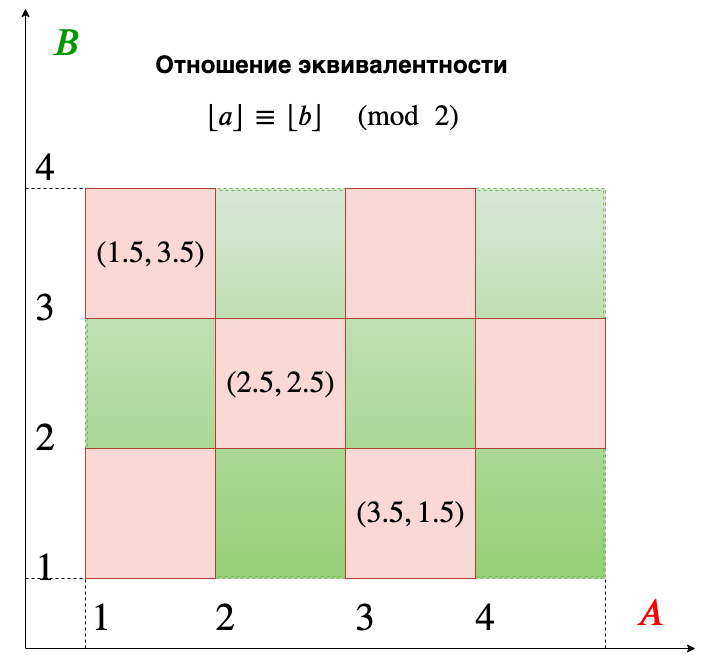
\includegraphics[scale=0.25]{equiv.png}
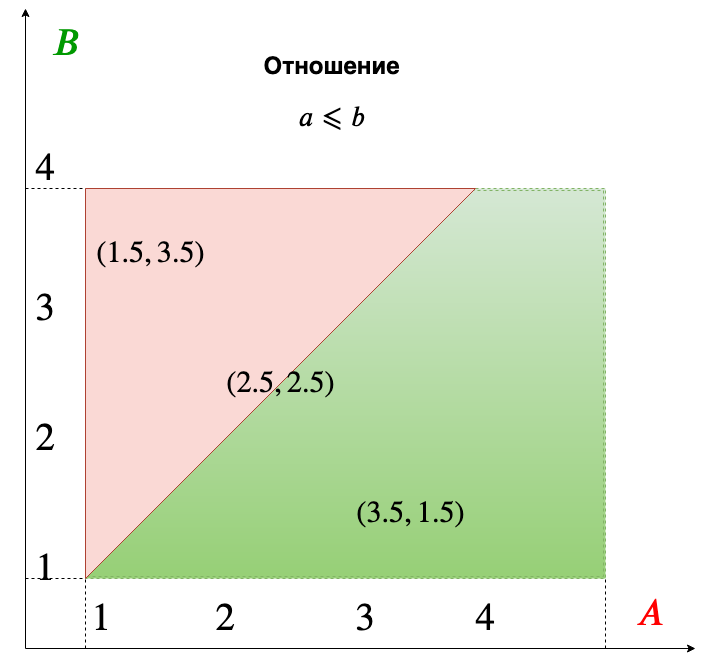
\includegraphics[scale=0.25]{lessthan.png}
\end{center}




\newchapter{Перестановки}\label{Permutations}

\vrezka{
В этой главе мы в основном изучаем конечные группы на примере перестановок. Кроме того, изучаются некоторые свойства групп и вводятся необходимые теоретико-множественные определения.
}


\section{*Теория множеств: функции}\label{functions}

\lesson{Функция как отношение, инъекция, сюръекция, биекция. Область определения, область значений. Образ и прообраз множества. Обратная функция}

\begin{enumerate}
\item Введем понятие функции. Пусть у нас имеется отношение $F$ между множествами $X$ и $Y$. Отношение $F$ называется
\begin{enumerate}[{\bf Func1}]
\item \textbf{всюду значным}, если для каждого $y\in Y$ найдется $x\in X$ такое, что $xFy$;
\item \textbf{всюду определенным}, если для каждого $x\in X$ найдется $y\in Y$ такое, что $xFy$;
\item \textbf{однозначным}, если всякий раз из одновременного выполнения $xFy$ и $xFy'$ следует, что $y=y'$, т.е. каждому $x$ соответствует не более одного $y$;
\item \textbf{обратно однозначным}, если всякий раз из одновременного выполнения $xFy$ и $x'Fy$ следует, что $x=x'$, т.е. каждому $y$ соответствует не более одного $x$;
\item \textbf{функцией из $X$ в $Y$}, если оно всюду определенное и однозначное;\index{Функция}
\item \textbf{частичной функцией из $X$ в $Y$}, если оно однозначное;
\item (частичной) \textbf{сюръекцией из $X$ на $Y$}, если это всюду значимая (частичная) функция;\index{Функция!сюръекция}
\item (частичной) \textbf{инъекцией из $X$ в $Y$}, если это обратно однозначная (частичная) функция;\index{Функция!инъекция}
\item \textbf{биекцией множеств $X$ и $Y$}, если это инъекция и сюръекция одновременно, т.е. отношение $F$ в данном случае взаимно однозначно связывает пары $(x,y)$.\index{Функция!биекция}
\end{enumerate}
\begin{center}
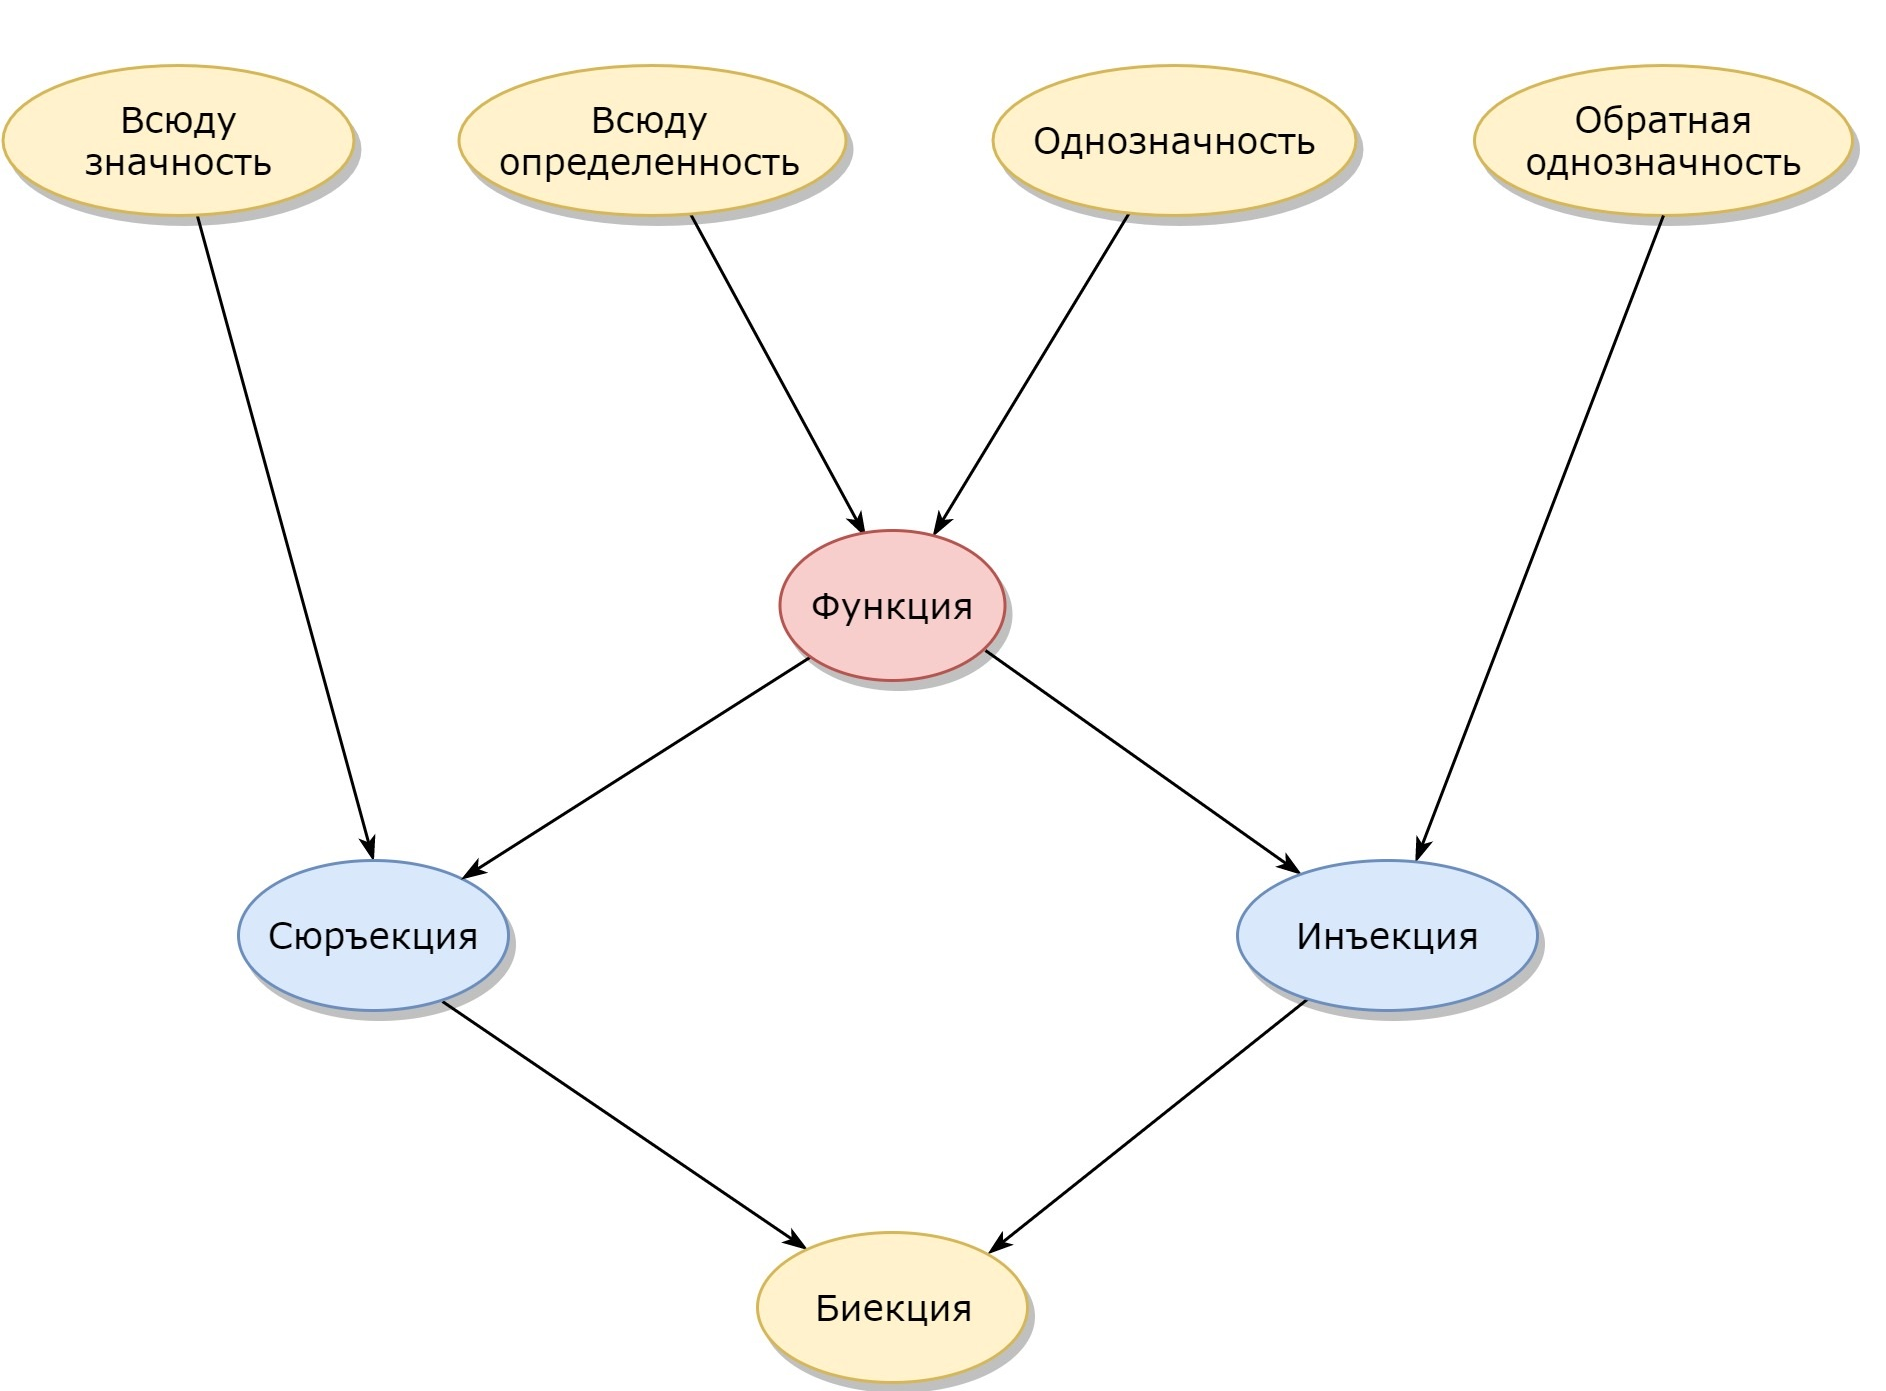
\includegraphics[scale=0.3]{function.png}
\end{center}


Обычно функция из $X$ в $Y$ обозначается $F:X\to Y$, а если $xFy$, то пишут $y=F(x)$. Для обозначения биекции часто используется символ $F:X\leftrightarrow Y$.
\item Обратным к $F$ отношением называется отношение $F^{-1}=\{(y,x)\mid xFy\}$. Если обратное отношение есть (частичная) функция, то она называется \textbf{обратной функцией}. Легко видеть, что $F(F^{-1}(y))=y$ и $F^{-1}(F(x))=x$, если только $F(x)$ и $F^{-1}(y)$ определены.
\item \textbf{Областью определения} функции $F$ называется множество $X$, а областью \textbf{определения частичной функции} $F$ --- подмножество $X$, для элементов которого $F$ определена, \textbf{областью значений} (частичной) функции $F$ называется подмножество $Y$, для элементов которого $F$ определена.
\item \textbf{Образом} множества $A\subseteq X$ относительно функции $F$ называется множество\index{Образ}
$$
F[A] = \{y\mid \exists x\in X\;y=F(x)\},
$$
т.е. образ множества --- это результат действия на него функции $F$.

Соответственно, \textbf{прообразом} множества $B\subseteq Y$ называется\index{Прообраз}
$$
F^{-1}[Y] = \{x\mid F(x)\in Y\},
$$
т.е. прообраз множества --- это такое множество исходных точек, образ которого лежит в данном множестве $Y$. Заметим, что для существования прообраза не требуется существования орбратной функции. Кроме того, заметим, что $F[F^{Y}]$ не всегда равен $Y$.
\item Итак, функция --- это есть однозначное соответствие элементов одного множества элементам другого (или того же самого). Функции обычно задаются формулами, предписывающими некоторой алгоритм вычисления $y$ через $x$. Но иногда такие формулы не указаны явно или же их указать вовсе невозможно, хотя существование функции строго доказывается (такие теоремы называют теоремами существования).
\end{enumerate}

\subsection*{Задачи}
\begin{enumerate}
\item Рассмотрим соответствие множества людей и множества всех возрастов (целых лет). В каком направлении соответствие между ними является функцией?
\item Рассмотрим соответствие множества людей и банковских счетов. Является ли это соответствие функцией хоть в каком-то направлении?
\item Докажите, что $F[A\cup C]=F[A]\cup F[C]$ и $F^{-1}[A\cup C]=F^{-1}[A]\cup F^{-1}[C]$.
\item Докажите, что $F[A\cup C]\subseteq F[A]\cup F[C]$ и $F^{-1}[A\cup C]=F^{-1}[A]\cup F^{-1}[C]$.
\item Привести примеры, когда $F[A\cup C]\ne F[A]\cup F[C]$.
\end{enumerate}


\section{Конечные группы}

\lesson{Повторение: группы. Единственность единицы и обратного элемента, порядок элемента, система образующих, циклическая группа}

\begin{enumerate}
\item Рассмотрим группу $G$, состоящую из $n$ элементов, с операцией $\cdot$ (обозначение которой часто будем пропускать для удобства). В терминах функций операция $\cdot$ есть функция из $G\times G$ в $G$:
$$
\cdot: G\times G\to G.
$$

Напомним аксиомы группы:\index{Группа}
\begin{enumerate}[G1]
\item $ab\in G$ для всех $a,b\in G$ (группоид);
\item для любых $a,b,c\in G$ имеем тождество $(ab)c=a(bc)$ (ассоциативность);
\item существует элемент $\e\in G$ такой, что $a\e=\e a=a$ для всех $a\in G$ (единица);
\item для всякого $a\in G$ существует обратный элемент $a^{-1}\in G$ такой, что $aa^{-1}=a^{-1}a=\e$ (обратный элемент).
\end{enumerate}
Кроме того, группа называется абелевой (или коммутативной), если $ab=ba$ для всех $a,b\in G$. Количество элементов в группе называется ее порядком.
\item В группе существует только одна единица. Действительно, если их две $\e$ и $\e'$, то в силу их же свойств получим
$$
\e' = \e\e' = \e
$$
(при первом равенстве мы рассматривали $\e$ как единицу, а при втором $\e'$).
\item Обратный элемент для каждого $a\in G$ определен однозначно. Предположим, что для элемента $a$ нашлось два обратных элемента $b,c$, т.е. $ab=ba=\e$ и $ac=ca=\e$. Тогда
$$
b=b\e=b(ac)=(ba)c=\e c=c.
$$
\item Степень элемента $\underbrace{a\cdots a}_{k\mbox{ раз}}$ обозначается $a^k$, где $k\in\N$. Кроме того, по определению, $a^0=\e$.
\item Отрицательная степень элемента по определению: $a^{-k}=(a^{-1})^k$, $k\in\N$.
\item Операции над степенями:
$$
(a^k)(a^m)=a^{k+m},
$$
где $k,m\in Z$. Если $k$ и $m$ одного знака, то это очевидно, а если разного, то пусть $k>0$, $m<0$, тогда
$$
(a^k)(a^m) = \underbrace{a\cdots a}_{k\mbox{ раз}}\underbrace{a^{-1}\cdots a^{-1}}_{|m|\mbox{ раз}}.
$$
Пользуясь ассоциативностью, начинаем сворачивать пары $aa^{-1}$, стоящие в середине, заменяя их на $\e$, а затем выбрасывая $\e$. В итоге либо ничего не останется (когда $k=-m$), либо останутся только $a$ в количестве $k+m$ (если $k>-m$), либо останутся только $a^{-1}$ в количестве $-m-k$ (когда $k<-m$). В любом случае это записывается как $a^{k+m}$ ($(a^{-1})^{-m-k}=a^{m+k}$ по определению).

\item В конечной группе каждый элемент в некоторой конечной степени обращается в $\e$. Действительно, все степени $a^k$ лежат в конечном множестве $G$, а число $k$ пробегает бесконечный науральный ряд. Следовательно, хотя бы два разных $k$ дадут один и тот же элемент (принцип Дирихле): $a^k=a^{k'}$, где $k<k'$. Домножим это равенство на $a^{-k}$ и получим $a^{k'-k}=\e$. Наименьший положительный показатель степени $m$ для элемента $a$, дающий равенство $a^m=\e$, называется порядком элемента $a$ в группе $G$.

Таким образом, в конечной группе у всякого элемента конечный порядок.

\item Отсюда следует, что всякую отрицательную степень элемента в конечной группе можно записать как положительную, поскольку
$$
a^k = a^{k\pmod p},
$$
где $p$ --- порядок элемента $a$.

\item Подмножество $T\subseteq G$, все возможные произведения степеней элементов которого, т.е. выражения вида $t_1^{k_1}\cdots t_m^{k_m}$, где $t_j\in T, k_j\in\N$ , образуют всю группу $G$, называется \textbf{системой образующих}\index{Группа!система образующих} или \textbf{порождающим множеством} группы $G$. При этом пишут $G=\langle T\rangle$ или $G=\langle t_1,\dots,t_m\rangle$. Элементы системы образующих называются \textbf{образующими} группы.
\item Если система образующих состоит из одного нетривиального элемента, то группа называется \textbf{циклической}.\index{Группа!циклическая} При этом ее можно записать так: $G=\langle g\rangle$, где $T=\{g\}$. Иначе говоря, циклическая группа состоит из степеней одного своего элемента.
\item Например, группа $\Z_n$ вычетов по модулю $n$ с операцией сложения является циклической: $\Z_n=\langle 1\rangle$, поскольку все ее элементы --- это конечные суммы единиц (от одной до $n$ штук). Группа вращений правильного $n$-угольника является циклической, где образующим элементом является поворот на угол $2\pi/n$. Группа $\Z_5^*$ с операцией умножения по модулю 5 является циклической вида $\langle 2\rangle$ и $\langle 3\rangle$.
\item Циклические группы являются абелевыми. Действительно, любые два элемента такой группы --- это некоторые степени образующего элемента, поэтому $(a^k)(a^m)=a^{k+m}=a^{m+k}=(a^m)(a^k)$. Коммутативность наследуется от группы $\Z$.


\lesson{Подгруппа, классы смежности, теорема Лагранжа}


\item Подмножество $H\subseteq G$ называется подгруппой группы $G$, если $H$ само является группой с той же операцией, которая определена в $G$. Например, $\{0,2\}$ образует подгруппу группы $\Z_4$. Тривиальная подгруппа $\{\e\}$ является подгруппой любой группы.

\item Операции Минковского для подгруппы:
$$
gH=\{gh\mid h\in H\},\quad Hg=\{hg\mid h\in H\},
$$
где $gH$ называется левым, а $Hg$ --- правым классом смежности, порожденным элементом $g\in G$.

\item Классы смежности содержат одинаковое количество элементов.

Действительно, пусть $h_1\ne h_2$, где $h_1,h_2\in H$. Предположим, что $gh_1=gh_2$. Домножая слева на $g^{-1}$, находим, что $h_1=h_2$. Противоерчие. Следовательно, умножение на $g$ слева различные элементы переводит в различные. Аналогично --- для умнжения справа.

\item Классы смежности подгруппы $H$ либо совпадают, либо не пересекаются, а их объединение равно $G$. То есть, классы смежности образуют разбиение множества $G$. Такую ситуацию мы уже наблюдали в связи с подгруппами $m\Z$ и их сдвигами внутри $\Z$ и получали там $m$ классов смежности.

Пусть классы $g_1H$ и $g_2H$ имеют общий элемент $g$. Этот элемент будет иметь два представления: $g=g_1h_1=g_2h_2$, где $h_1,h_2\in H$, откуда $g_1=g_2h_2(h_1)^{-1}$. Возмем любой элемент $g_1h$ из первого класса, тогда
$$
g_1h = g_2h_2(h_1)^{-1}h,
$$
где $h_2(h_1)^{-1}h\in H$, т.к. $H$ --- подгруппа. Следовательно, $g_1h\in g_2H$, и $g_1H\subseteq g_2H$. Аналогично рассуждая, находим, что $g_2H\subseteq g_1H$, т.е. $g_1H=g_2H$.

Тот факт, что любой элемент $G$ находится в каком-то классе смежности, следует из того, что $\e\in H$, так что для любого $g\in G$ имеем $g\in gH$. И аналогично для правых классов.

\item Итак, множество $G$ есть сумма непересекающихся классов одного размера, причем размер классов равен порядку подгруппы $H$. Следовательно, порядок подгруппы делит подрядок группы. Это утверждение называется \textbf{теоремой Лагранжа}.\index{Теорема!Лагранжа о порядке группы}

\item $g_1H=g_2H$ тогда и только тогда, когда $(g_1)^{-1}g_2\in H$.

Пусть $g_1H=g_2H$, тогда любой элемент из этого множества имеет представление $g_1h_1=g_2h_2$, откуда $h_1(h_2)^{-1}=(g_1)^{-1}g_2$. Элемент слева --- это элемент подгруппы $H$.

Обратно, пусть $(g_1)^{-1}g_2=h\in H$, тогда $g_1h=g_2\e$. Элемент слева принадлежит $g_1H$, элемент справа --- $g_2H$, т.е. эти классы имеют общий элемент, а значит, совпадают.

\item Если группа имеет порядок $p$, где $p$ простое число, то такая группа является циклической.

Действительно, возьмем элемент $g\ne\e$ (поскольку $p>1$, то такое всегда возможно). Пусть $H=\langle g\rangle$ --- циклическая подгруппа $G$. Ее порядок делит порядок группы $G$, т.е. простое число $p$. В то же время, порядок $H$ отличен от 1, т.к. $H$ содержит как минимум два элемента $\e,g$. Но так как $p$ делится только на 1 и на $p$, то порядок группы $H$ равен $p$. Следовательно, $G=\langle g\rangle$.


\lesson{Нормальная подгруппа, факторгруппа, изоморфизм. Примеры: $\Z_2\times\Z_2$ и $\Z_8^*$}


\item Подгруппа $H$ группы $G$ называется \textbf{нормальной}\index{Группа!нормальная подгруппа}, если для любого $g\in G$ верно равенство $gH=Hg$, т.е. левые и правые классы не различаются. Обозначение: $H\vartriangleleft G$.

В абелевых группах любая подгруппа будет нормальной. В частности, $m\Z$ --- нормальная в $\Z$.

\item Следующее вложение является как критерием нормальной подгруппы, так и, зачастую, используется в качестве ее определения:
\begin{equation}\label{normcriteria}
g^{-1}Hg\subseteq H,\quad (gHg^{-1}\subseteq H).
\end{equation}

Неравенство в скобках равносильно первому, поскольку $g$ --- произвольный элемент $G$, а значит, вместо него можно подставить ему обратный.

Проверим этот критерий. Пусть $H$ --- подгруппа $G$, и выполнено тождество $gH=Hg$ для всех $g\in G$. В частности, это значит, что $Hg\subseteq gH$, т.е.
$$
\forall g\;\forall h\;\exists h'\;(hg=gh')
$$
(не обязательно $h'=h$). Домножая это равенство слева на $g^{-1}$, получаем $g^{-1}hg=h'$, т.е.
$$
\forall g\;\forall h\;(g^{-1}hg\in H),
$$
т.е. $g^{-1}Hg\subseteq H$.

Обратно. Пусть выполнено вложение $g^{-1}Hg\subseteq H$. То есть, для любых $g\in G$ и $h\in H$ найдется такой $h'\in H$, что $g^{-1}hg=h'$, откуда умножением слева на $g$ получаем $hg=gh'$. Откуда следует, что $Hg\subseteq gH$.

С другой стороны, $gHg^{-1}\subseteq H$, откуда следует, что для любых $g\in G$ и $h\in H$ найдется такой $h'\in H$, что $ghg^{-1}=h'$, откуда умножением справа на $g$ получаем $gh=h'g$. Откуда следует, что $gH\subseteq Hg$. Окончательно получаем $gH=Hg$.

\item Условие \eqref{normcriteria} равносильно равенству
$$
g^{-1}Hg=H.
$$
Действительно, из этого равенства автоматически следует \eqref{normcriteria}. Поэтому необходимо показать обратное. Выше мы показали, что из \eqref{normcriteria} следует $gH=Hg$. Пусть $h\in H$, тогда
$$
h=(g^{-1}g)h(g^{-1}g)=g^{-1}(ghg^{-1})g=g^{-1}h'g\in g^{-1}Hg,\quad h'\in H,
$$
где $h'\in H$ в силу вложения $gHg^{-1}\subseteq H$. Таким образом, $H\subseteq g^{-1}Hg$, что вместе с вложением \eqref{normcriteria} дает равенство $g^{-1}Hg=H$.


\item Классы смежности нормальной подгруппы можно умножать так же, как сами элементы группы $G$:
$$
(g_1H)(g_2H)=(g_1g_2)H.
$$
Это следует из того, что $(g_1h_1)(g_2h_2)=g_1(h_1g_2)h_2$, и при этом $h_1g_2=g_2h_3$ при некотором $h_3$ в силу нормальности $H$. Следовательно,
$$
(g_1h_1)(g_2h_2) = g_1(h_1g_2)h_2 = g_1(g_2h_3)h_2=(g_1g_2)(h_3h_2)\in (g_1g_2)H.
$$
Обратно, $(g_1g_2)h=(g_1\e)(g_2h)$. Здесь первый множитель принадлежит $g_1H$, второй $g_2H$. Так что мы имеем взаимное вложение множеств $(g_1H)(g_2H)$, $(g_1g_2)H$, т.е. их равенство.

\item Такое свойство умножения классов смежности по нормальной подгруппе позволяет задать групповую операцию на множестве всех классов смежности, которое обозначается
$$
G/H = \{gH\mid g\in G\}
$$
и называется \textbf{фактор-группой}\index{Группа!Фактор-группа} группы $G$ по нормальной подгруппе $H$. Опять же, мы уже сталкивались с примером фактор-группы $\Z/m\Z$ при изучении группы вычетов (см. раздел \ref{Faktor})

\item Факторизацию группы можно воспринимать как делимость групп, и в этом смысле группы становятся подобны числам. Есть простые группы --- они ни на что не делятся, а есть составные --- они делятся на нормальные подгруппы.

\item Естественно ввести и умножение групп. Пусть даны две группы $G_1$ и $G_2$ с операциями $\circ$ и $\star$, соответственно. Тогда на прямом произведении $G_1\times G_2$ определим операцию умножения по правилу
$$
(g_1,g_2)(g_1',g_2') = (g_1\circ g_1', g_2\star g_2'),
$$
т.е. будем покомпонентно перемножать все пары элементов прямого произведения. Легко проверить, что это --- групповая операция, т.е. она ассоциативна, имеет единицу, а для каждой пары есть обратная. Все эти свойства наследуются от исходных групп напрямую. Кроме того, если исходные группы абелевы, то и произведение групп будет абелевой группой. Такая конструкция называется внешним \textbf{прямым произведением групп} $G_1$ и $G_2$.

Если в исходных группах операция интерпретируется как сложение, то прямое произведение называют прямой суммой групп. Но, учитывая, что это может привести к путанице понятий, мы в любом случае будем пользоваться мультипликативной терминологией и символикой. Тем более, что она согласуется с теоретико-множественным прямым произведением.

\item Рассмотрим простой пример произведения групп: $\Z_2\times\Z_2$. Вот ее таблица умножения:

\begin{center}
\begin{tabular}{c|cccc}
$\Z_2\times\Z_2$ & 00 & 01 & 10 & 11\\  \hline
00 & 00 & 01 & 10 & 11 \\
01 & 01 & 00 & 11 & 10 \\
10 & 10 & 11 & 00 & 01 \\
11 & 11 & 10 & 01 & 00
\end{tabular}
\end{center}
где вместо пары $(i,j)$ мы просто пишем $ij$ для краткости.

Видим, что эта группа абелева, но не циклическая. В этой группе есть три подгруппы $\{00,01\}$, $\{00,10\}$ и $\{00,11\}$.

Если сравнить ее с группой $\Z_4$ по сложению, то мы увидим существенную разницу. Во-первых, в $\Z_4$ только одна подгруппа $\{0,2\}$, а во-вторых, $\Z_4$ является циклической группой.

Этот пример показывает нам, что порядок группы не определят однозначно ее структуру (как нам того бы хотелось, памятуя об основной теореме арифметики).

Однако, нам уже хорошо знакома группа, которая имеет такую же таблицу умножения, как и $\Z_2\times\Z_2$. Это все та же группа симметрий ромба, т.е. четверная группа Клейна. Чуть позже мы к ней вернемся.

\item Говорят, что функция $f:G_1\to G_2$ является \textbf{изоморфизмом}\index{Изоморфизм групп} групп $(G_1,\circ)$ и $(G_2,\star)$, если $f$ осуществляет взаимно однозначное соответствие обеих групп $g_2=f(g_1)$ так, что и результат операций в первой группе переходит в результат операций во второй:
$$
f(g_1\circ g_1') = f(g_1)\star f(g_1').
$$

Например, если мы рассмотрим группы $G_1=\Z_2\times\Z_2$ и $G_2=\Z_8^*$, то следующее соответствие
$$
01\mapsto 1,\quad 01\mapsto 3,\quad 10\mapsto 5, \quad 11\mapsto 7
$$
будет изоморфизмом этих групп. Это видно из следующих таблиц:

\begin{center}
\begin{tabular}{c|cccc}
$\Z_8^*$ & 1 & 3 & \cellcolor{lightRed} 5 & 7 \\  \hline
1 & 1 & 3 & 5 & 7 \\
3 & 3 & 1 & 7 & 5\\
5 & 5 & 7 & 1 & 3\\
7 & 7 & \cellcolor{lightRed} 5 & 3 & 1
\end{tabular}
\qquad
\begin{tabular}{c|cccc}
$\Z_2\times\Z_2$ & 00 & 01 & \cellcolor{lightRed} 10 & 11\\  \hline
00 & 00 & 01 & 10 & 11 \\
01 & 01 & 00 & 11 & 10 \\
10 & 10 & 11 & 00 & 01 \\
11 & 11 & \cellcolor{lightRed} 10 & 01 & 00
\end{tabular}
\end{center}

\end{enumerate}





\section{Арифметика перестановок}

\lesson{Перестановка, группа перестановок, порядок группы пеерестановок. Теорема Кэли. Обозначения перестановок}

\begin{enumerate}
\item Рассмотрим множество $X_n=\{x_1,\dots,x_n\}$, состоящее из $n$ элементов. На этом множестве рассмотрим все возможные биекции множества $X_n$ в себя. Обозначим
$$
\Sb(X_n) = \{f\mid f:X_n\leftrightarrow X_n\},
$$
проще говоря, это множество всех возможных \textbf{перестановок} элементов множества $X_n$.
\item Для функций, заданных на множестве, естественной операцией является операция композиции, т.е. последовательное применение функций друг к другу. Обычно композиция функций записывается символом $\circ$ или пропускается как умножение. Мы будем пользоваться первым вариантом, так что:
$$
(f\circ g)(x) = f(g(x))
$$
по определению.
\item Итак, мы имеем множество биекций (перестановок) с операцией композиции. Свойства композиции биекций таковы:
\begin{enumerate}[1.]
\item композиция биекций есть снова биекция;
\item $f\circ (g\circ h) = (f\circ g)\circ h$, поскольку это последовательное вычисление $f(g(h(x)))$;
\item существует функция, которая ничего не меняет: $\id(x)=x$, она также является биекцией;
\item для всякой биекции существует обратная функция, которая также является биекцией: $f\circ f^{-1}=f^{-1}\circ f=\id$;
\end{enumerate}

Таким образом, множество $\Sb(X_n)$ (и вообще, для любого множества $X$) с операцией композиции является группой. Эта группа называется \textbf{группой перестановок}\index{Группа!перестановок} множества $X_n$, а ее элементы--биекции называются \textbf{перестановками} (или подстановками).\index{Перестановка}
\item Один простой пример такой группы перестановок мы уже встречали, когда рассматривали все возможные симметрии правильного треугольника. Именно в этом случае все перестановки вершин треугольника оказались движениями, и только они.
\item Сколько всего перестановок в группе $\Sb(X_n)$?

Для ответа на этот вопрос посмотрим, сколько существует вариантов перехода одних элементов в другие. Очевидно, что первый элемент может перейти в любой, в том числе в самого себя, так что для него существует $n$ вариантов. Второй элемент может перейти куда угодно, кроме того места, которое занял первый, так что для него существует $n-1$ вариант. Третьему остается $n-2$ варианта. И т.д. Последнему элементу остается выбор из одного оставшегося места. Таким образом, всего вариантов перестановок на $n$ элементах существует ровно
$$
n(n-1)(n-2)\dots 2\cdot 1=n!
$$
Иначе говоря, группа $\Sb(X_n)$ имеет порядок $n!$.

\item Группа перестановок на 3х элементах имеет порядок $3!=6$, что соответствует количеству симметрий правильного треугольника.
Однако уже для квадрата число перестановок равно $24$, в то время как число всех движений составляет всего лишь 8, а для ромба так и вовсе 4. Вообще, как мы помним, количество движений правильного $n$-угольника равно $2n$. С ростом $n$ это число становится во много раз меньше, чем $n!$ (а точнее, в $3\cdot 4\cdots (n-1)=(n-1)!/2$ раз).
\item Чтобы не заострять внимание на происхождении элементов множества $X_n$, обычно они обозначаются числами от $1$ до $n$, так что $X_n=\{1,2,\dots, n\}$, а соответствующая группа биекций --- $\Sb_n$. Легко видеть, что группы $\Sb_n$ и $\Sb(X_n)$ изоморфны, т.е. между ними существует биекция, сохраняющая операцию композиции. Поэтому в дальнейшем, говоря о группе перестановок, мы будем иметь ввиду $\Sb_n$, заданную на множестве чисел $1,\dots, n$.
\item Теория групп в XIX в. начиналась именно с изучения групп подстановок, и лишь позже понятие группы было обобщено Артуром Кэли. Он же сделал первый важный шаг на пути классификации групп.
\begin{thrm}[Кэли]\index{Теорема!Кэли}
Любая конечная группа порядка $n$ изоморфна некоторой подгруппе $\Sb_n$.
\end{thrm}
Для доказательства достаточно заметить, что каждый элемент $g$ исходной группы $G$ порождает биекцию на $G$ по правилу $h\mapsto gh$ (<<правые>> биекции), а эти биекции образуют изоморфную $G$ подгруппу внутри группы биекций на $G$.
\item В группе $\Sb_n$, как и в любой другой, можно построить циклическую подгруппу, отправляясь от произвольно взятого элемента, т.\,е. биекции на $X_n$. Например, пусть $s\in\Sb_n$, тогда можно рассмотреть циклическую подгруппу $G(s)=\{s,s^2,s^3,\dots\}$, где под степенью понимается многократная композиция биекции $s$ с самою собой. Ясно, что эта подгруппа не может быть бесконечной, т.\,к. она входит в конечную группу, поэтому при некотором $k$ имеем $s^k=\id$.

\item Рассмотрим некоторую перестановку $s\in \Sb_n$. Ее можно записать в виде таблицы аргумент--значение:
$$
s=
\begin{pmatrix}
1 & 2 & \dots & n-1 & n \\
s_1 & s_2 & \dots & s_{n-1} & s_n
\end{pmatrix}
$$
т.\,е. $s(i)=s_i$. При этом $\{1,2,\dots,n\}=\{s_1,s_2,\dots,s_n\}$ в полном соответствии с определением равенства множеств.

\item Возьмем теперь элемент 1 и начнем <<раскручивать>> его так же, как мы <<раскручивали>> степени элемента в циклической группе:
$$
1\mapsto s(1)\mapsto s(s(1))\mapsto\dots\mapsto s^k(1)
$$
Мы получим то, что называется \textbf{орбитой} элемента 1 при действии группы $G(s)$ на множестве $X_n$. Действительно, все элементы данной цепочки составляют множество $G(s)1=\{g(1)|\;g\in G(s)\}$. Кроме того, если $s^k=\id$, то $s^k(1)=1$, и мы получаем \textbf{цикл}:
$$
(1\; s(1)\; s(s(1))\;\dots\; s^{k-1}(1))
$$
(единицу в конце мы не пишем, подразумевая, что последний элемент цикла переходит в первый).

\item Действие группы $G(s)$ на множестве $X_n$ позволяет разбить это множество на несколько попарно непересекающихся орбит или циклов. Отсюда мы получаем представление самой перестановки $s$ как набора независимых циклов. Поэтому перестановки принято записывать в виде последовательности циклов. Например, пусть
$$
s=
\begin{pmatrix}
1 & 2 & 3 & 4 & 5 \\
2 & 4 & 1 & 3 & 5
\end{pmatrix}
$$
В этой перестановке мы наблюдаем два цикла: $(1 2 4 3)$ и тривильный $(5)$. Тогда
$$
s=(1 2 4 3)(5),
$$
причем, тривиальные циклы принято пропускать в такой <<циклической>> записи, т.\,к. они однозначно восстанавливаются по всем остальным циклам и по параметру $n$ (в нашем случае $n=5$).
\item Рассмотрим более сложный пример:
$$
s=
\begin{pmatrix}
1 & 2 & 3 & 4 & 5 & 6 & 7 \\
2 & 4 & 3 & 1 & 7 & 5 & 6
\end{pmatrix}
=(1 2 4)(3)(5 7 6)=(1 2 4)(5 7 6)
$$

\item Предположим теперь, что у нас имеется три перестановки:
$$
s_1=
\begin{pmatrix}
1 & 2 & 4 \\
2 & 4 & 1
\end{pmatrix}
\quad s_2=
\begin{pmatrix}
5 & 6 & 7 \\
7 & 5 & 6
\end{pmatrix}
\quad s_3=\id
$$
Тогда исходная перестановка $s$ получается как последовательное применение этих новых перестановок:
$$
s=s_1s_2s_3,
$$
причем порядок перестановок в композиции неважен, т.\,к. две из них <<работают>> на разных орбитах, а третья тождественна и коммутирует с любой перестановкой.

\item Таким образом, каждую перестановку из $\Sb_n$ можно единственным образом (с точностью до порядка) представить как композицию циклов, и, таким образом, запись перестановки в виде набора ее циклов является не только удобным соглашением, но еще и функционально верной.


\lesson{Транспозиция. Теорема о четности перестановки. Гомоморфизм, ядро. Основная тоерема о гомоморфизмах}


\item Наконец, введем такое понятие как \textbf{транспозиция}. Это --- микроцикл, состоящий из двух элементов, например, (12) или (59) и т.п. Транспозиция меняет местами два элемента $X_n$, а остальные оставляет на месте. Любой цикл длины $k$ можно представить как композицию $k-1$ транспозиции. Например,\label{transpose}\index{Транспозиция}
$$
(1234) = (14)(13)(12),
$$
причем, это представление неоднозначное, поскольку:
$$
(2341) = (21)(24)(23),
$$
тем не менее, любая перестановка (не только цикл) имеет \textit{инвариант} по разложению в транспозиции.
\begin{thrm}
Если перестановка $g\in\Sb_n$ имеет два представления транспозициями
$$
t_1\dots t_k=g=\tau_1\dots\tau_m,
$$
то $k\equiv m\mod 2$.
\end{thrm}
Иначе говоря, четность перестановки, определяемая количеством входящих в ее разложение транспозиций, не зависит от способа этого разложения. Величина $\sgn(g)=(-1)^k=(-1)^m$ называется \textbf{знаком перестановки} $g$.

\item Функция $\sgn$, определенная на элементах группы $\Sb_n$ и принимающая значения из множества $B=\{-1,1\}$, является гомоморфизмом групп $\Sb_n$ и $B$ (проверьте, что $(B,\cdot)$ есть группа по умножению, изоморфная $\Z_2$).

\item В связи с этим дадим общее определение: \textbf{гомоморфизмом групп} $(G,\cdot)$ и $(G',\circ)$ называется всякая функция $h:G\to G'$, сохраняющая групповую операцию, т.\,е. $$h(g_1\cdot g_2)=h(g_1)\circ h(g_2).$$

Изоморфизм --- частный случай гомоморфизма. Ядром гомоморфизма $h$ называется прообраз единицы:
$$
\Ker(h)\rightleftharpoons h^{-1}\{\e'\}\rightleftharpoons\{g\in G|\;h(g)=\e'\},
$$
где $\e'$ --- единица группы $G'$.

Гомоморфизм обладает слеюущими свойствами
\begin{enumerate}[\bf Hom1]
\item Гомоморфизм единицу переводит в единицу. Действительно, пусть $h(\e)=g'$. Тогда
$$
g'=h(\e)=h(\e\e)=h(\e)h(\e)=g'g',
$$
откуда, используя сокращение в группе $G'$, получаем, что $\e'=g'$.

\item Гомоморфизм обртаный элемент переводит в обратный. Пусть $g'=h(g)$ и $g''=h(g^{-1})$, тогда
$$
g'g'' = h(g)h(g^{-1})=h(gg^{-1})=h(\e)=\e',\quad g''g'=\e',
$$
т.е. элемент $g''$ --- обратный к $g'$, т.е. $h(g^{-1})=h(g)^{-1}$.

\item Ядро гомоморфизма есть нормальная подгруппа: $\Ker(h)\vartriangleleft G$.

Проверим аксиомы группы. Пусть $g_1, g_2\in G$, тогда $h(g_1g_2)=h(g_1)h(g_2)=\e'$, откуда $g_1g_2\in\Ker(h)$, т.е. ядро замкнуто относительно групповой операции в $G$. Ассоциативность в ядре не зависит от гомоморфизма, она наследуется из $G$. Единица также остается единицей и в ядре.

Пусть $g\in\Ker(h)$, тогда $h(g^{-1})=h(g)^{-1}=(\e')^{-1}=\e'$, откуда $g^{-1}\in\Ker(h)$. Таким образом, все требования группы выполнены. $\Ker(h)$ является группой. Проверим ее нормальность.

Пусть $g\in G$ и $k\in\Ker(h)$, тогда $h(g^{-1}kg)=h(g)^{-1}h(k)h(g)=h(g)^{-1}\e'h(g)=\e'$. Отсюда следует, что $g^{-1}kg\in\Ker(h)$, т.е. $g^{-1}\Ker(h)g\subseteq \Ker(h)$.

А это, по доказанному ранее критерию нормальности, означает, что $\Ker(h)\vartriangleleft G$.

\end{enumerate}

\item Поскольку функция $\sgn$ на группе $\Sb_n$ действует как гомоморфизм в группу $B$, прообраз 1 в группе $\Sb_n$ относительно данного гомоморфизма, а именно, \textit{все четные перестановки} образуют нормальную подгруппу в группе подстановок $\Sb_n$. Эта нормальная подгруппа обозначается $A_n$ и называется \textbf{знакопеременной группой}\index{Группа!знакопеременная} порядка $n$. Не следует путать употребленное здесь слово <<порядок>> с порядком группы, означающим количество ее элементов, поскольку в $A_n$ находится ровно половина элементов группы $\Sb_n$, т.\,е. $n!/2$, что значительно больше $n$.

\item О тесной связи гомоморфизмов и нормальных групп говорит следующая

\begin{thrm}[Основная теорема о гомоморфизмах групп]\index{Теорема!основная о гомоморфизмах}
Пусть $h:G\to G'$ --- гомоморфизм, тогда
фактор-группа $G/\Ker(h)$ изоморфна области значений $h$ в группе $G'$. Наоборот, если $H\vartriangleleft G$, то существует гомоморфизм $h:G\to G/H$ такой, что $H=\Ker(h)$.
\end{thrm}
\hard{
\pf
Обозначим $K=\Ker(h)$, а область значений $h$ в группе $G'$ обозначим за $H'$. Необходимо построить изоморфизм между $G/K$ и $H'$.

Положим $f(gK)=h(g)$. Для начала необходимо показать корректность такого определения, а точнее, однозначность $f$, т.е. что значение $f$ не зависит от выбора представителя класса смежности $gK$.
Пусть $g_1K=g_2K$, т.е. $g_1k=g_2k'$ при некоторых $k,k'\in K$. Тогда $h(g_1k)=h(g_1)h(k)=h(g_1)$ и $h(g_2k')=h(g_2)h(k')=h(g_2)$, откуда $h(g_1)=h(g_2)$, т.е. $f$ определено корректно.

Далее, $f$ является сюръекцией на множество $H'$, поскольку для всякого $h'\in H'$ существует $g$ такой, что $h(g)=h'$, следовательно, $f(gK)=h'$.

Кроме того, $f$ является инъекцией в $H'$. Действительно, если $f(g_1K)=f(g_2K)$, то $h(g_1)=h(g_2)$, откуда следует, что $g_1g_2^{-1}\in K$. Но тогда $g_1=kg_2$ при некотором $k\in K$, т.е. $g_1\in Kg_2=g_2K$ (последнее равенство следует из нормальности $K$). Но тогда $g_1K\cap g_2K\ne\emptyset$, а значит, эти классы равны. Следовательно, $f$ --- инъекция.

Таким образом, $f$ --- биекция между $G/K$ и $H'$. Осталось показать, что она сохраняется групповую операцию.
$$
f(g_1Kg_2K)=f(g_1g_2K)=h(g_1g_2)=h(g_1)h(g_2)=f(g_1K)f(g_2K).
$$
Итак, $f$ --- изоморфизм.

Пусть $H\vartriangleleft G$. Определим гомоморфизм из $G$ в $G/H$ следующим образом:
$$
h(g)=gH, \quad g\in G.
$$

$h$ сохраняет групповую операцию, т.к. $h(g_1g_2)=(g_1g_2)H=(g_1H)(g_2H)=h(g_1)h(g_2)$. Поскольку единицей группы $G/H$ является $H$, очевидно, что $\Ker(h)=H$.
\epf}



\lesson{Сопряженные элементы. Автоморфизмы, классы сопряженности, критерий нормальности}

\item Пусть $g,x\in G$, где $G$ --- группа. Элемент $x^{-1}gx$ называется \textbf{сопряженным} к элементу $g$ при помощи $x$. Если сопряженный элемент обозначить как $g^x$, то у нас получаются знакомые свойства:
\begin{enumerate}[1)]
\item $g^{xy}=(g^x)^y$;
\item $(g_1g_2)^x=g_1^xg_2^x$;
\item $(g^{-1})^x=(g^x)^{-1}$;
\end{enumerate}

\begin{lem} Скажем, что $g_1\sim_G g_2$, если при некотором $x$ имеет место равенство $g_1^x=g_2$. Отношение $\sim$ является отношением эквивалентности.
\end{lem}
\pf Рефлексивность: $g=g^\e$. Симметричность: если $g_1^x=g_2$, то $g_2^{x^{-1}}=g_1$. Транзитивность: если $g_1^x=g_2$ и $g_2^y=g_3$, то $g_1^{xy}=g_3$.
\epf

Таким образом, группа $G$ разбивается на классы эквивалентности по отношению $\sim_G$, которые называются \textbf{классами сопряженности}. Класс сопряженности элемента $g$ обозначается $g^G$. Это --- возведение в степень по Минковскому, т.е.
$$
g^G=\{g^x\mid x\in G\}.
$$

\begin{lem} $g^x$ при фиксированном $x$ является изоморфизмом $G\leftrightarrow G$.
\end{lem}
\pf
Во-первых, $f(g)=g^x$ сохраняет операцию группы $G$, поскольку $f(g_1g_2)=f(g_1)f(g_2)$. Во-вторых, это мономорфизм (инъекция с сохранением операции), т.е. если $x^{-1}g_1x=x^{-1}g_2x$, то $g_1=g_2$. В-третьих, это эпиморфизм (сюръекция с сохранением операции), т.к. для любого $g\in G$ найдется $g'=xgx^{-1}$ такой, что $g=f(g')$.
\epf

Итак, при каждом $x$ функция $f(g)=g^x$ является изоморфизмом группы $G$ на себя. Такой изоморфизм называется \textbf{автоморфизмом} группы $G$.\index{Автоморфизм группы}

\item Посмотрим, как работает отношение сопряженности на группе перестановок.

Пусть $G=\Sb_3 = \{\id,(12),(13),(23),(123),(132)\}$. Будем записывать действие $g^x$ в виде таблицы, похожей на таблицу умножения, предплагая, что на верхнюю строку мы действуем функцией $g^x$, где $x$ берется из левого столбца:
\begin{center}
\begin{tabular}{c|c|ccc|cc}
$x$&  $\id$	& (12)	& (13)	& (23)	& (123)	& (132) \\ \hline
$\id$&$\id$	& (12)	& (13)	& (23)	& (123)	& (132) \\
(12)& $\id$	& (12)	& (23)	& (13)	& (132)	& (123) \\
(13)& $\id$	& (23)	& (13)	& (12)	& (132)	& (123) \\
(23)& $\id$	& (13)	& (12)	& (23)	& (132)	& (123) \\
(123)&$\id$	& (23)	& (12)	& (13)	& (123)	& (132) \\
(132)&$\id$	& (13)	& (23)	& (12)	& (123)	& (132)
\end{tabular}
\end{center}
Видим, что когда $x$ есть транспозиция, она себя и $\id$ оставляет на месте, а остальные элементы переставляет местами, оставляя их в своих классах, т.е. транспозиции переходят в транспозиции, а 3-циклы в 3-циклы. Если же $x$ --- это 3-цикл, то транспозиции он перемешивает, ни одну не оставляя на месте, а 3-циклы и $\id$ сохраняет.

Коме того, каждая строка таблицы --- это перестановка элементов группы $\Sb_3$, т.е., по сути, элемент группы $\Sb(\Sb_3)$, изоморфной группе $\Sb_6$.

Все перестановки, получаемые сопряжением элементов, имеют строгие ограничения. Мы специально разделили таблицу на три части, включив в первую $\id$, во вторую --- транспозиции, а в третью --- 3-циклы. Такое разделение соответствует найденному нами выше 
разбиению на классы сопряженности по
отношению эквивалентности $\sim_G$ (в нашем случае это $\sim_{\Sb_3}$). И действительно, если смотреть теперь на столбцы таблицы, то мы заметим, что, меняя $x$, мы ходим только в пределах своего класса сопряженности!

Мы можем построить аналогичную таблицу для $\Sb_4$ и убедиться в том, что (a) каждая строка таблицы есть перестановка элементов $\Sb_4$ и (b) каждый столбец --- выборка с повторениями из соответствующих классов сопряженности. Таковыи классами для $\Sb_4$ являются классы одинаковой цикловой формы:

\begin{tabular}{c|l|c}
()    & $\id$ & 1 \\
(**)   & (12),(13),(14),(23),(24),(34) & 6 \\
(***)  & (123),(132),(124),(142),(134),(143),(234),(243) & 8\\
(**)(**) & (12)(34), (13)(24), (14)(23) & 3 \\
(****) & (1234),(1243),(1324),(1342),(1423),(1432) & 6
\end{tabular}


Эти классы можно обозначить как $\id^{\Sb_4}$, $(12)^{\Sb_4}$, $(123)^{\Sb_4}$, $[(12)(34)]^{\Sb_4}$, $(1234)^{\Sb_4}$.

\item Классы сопряженности напрямую связаны с нормальными подгруппами.
\begin{thrm}\index{Подгруппа!критерий нормальности}
Подгруппа $H$ группы $G$ является нормальной тогда и только тогда, когда она есть объединение нескольких классов сопряженности.
\end{thrm}
\pf
Пусть $H\vartriangleleft G$, тогда $H=x^{-1}Hx$ для любого $x\in G$. Тогда вместе с любым элементом $h\in H$ имеем вхождение всего класса $h^G\subseteq H$.

Обратно, пусть $H=g_1^G\cup\dots\cup g_n^G$. Тогда, поскольку операция сопряжения сохраняет классы сопряженности, получаем, что
$$
x^{-1}Hx=x^{-1}g_1^Gx\cup\dots\cup x^{-1}g_n^Gx =g_1^G\cup\dots\cup g_n^G=H,
$$
откуда следует, что подгруппа $H$ является нормальной.
\epf

Отметим, что просто любое объединение классов сопряженности не обязано быть подгруппой, а значит, и нормальной подгруппой. Однако, нормальные подгруппы следует искать только среди таких объединений. Важно, чтобы эти объединения оказались замкнутыми относительно групповой операции! Поэтому такое объединение должно включать как минимум тривиальный класс $\{\e\}$.


\lesson{Нормальные подгруппы групп $\Sb_3$ и $\Sb_4$. Ипостаси четверной группы Клейна}


\item В группе $\Sb_3$ есть только две возможности создать нетривиальную нормальную подгруппу: на основе класса $(12)^{\Sb_3}$ и на основе класса $(123)^{\Sb_3}$. Но в первом случае подгруппа не получается, поскольку $(12)(23)=(123)$ выходит из класса транспозиций. Зато второй случай позволяет создать подгруппу
$$
A_3 = \{\id,(123),(132)\},
$$
и по доказанной теореме она является нормальной.

\item В группе $\Sb_4$ возможностей сильно больше, но далеко не все они приводят к подгруппе. Вспомним, что порядок подгруппы делит порядок группы (теорема Лагранжа). Следовательно, собственные нетривиальные подгруппы $\Sb_4$ должны иметь порядок из множества $\{2,4,6,8,12\}$. А перечисленные выше классы сопряженности имеют размеры 1,6,8,3,6. И так как подгруппа должна включать класс $\{\id\}$, ее порядок может скадываться только следующими способами: $1+3$, $1+3+8$. И действительно, в группе $\Sb_4$ существует ровно две нетривиальные собственные подгруппы:
\begin{align*}
V_4 = & \{\id,(12)(34),(13)(24),(14)(23)\},\\
A_4 = & \{\id,(12)(34),(13)(24),(14)(23), \\
      & \;(123),(132),(124),(142),(134),(143),(234),(243)\}
\end{align*}
Первая --- это уже известная нам четверная группа Клейна, которая изоморфна группе симметрий ромба, группе $\Z_8^*$ и группе $\Z_2\times\Z_2$. Можно построить гомоморфизм из $\Sb_4$ в $\Sb_3$ с ядром $V_4$. У этого факта существует простое геометрическое доказательство. Дело в том, что группа $\Sb_4$ является группой симметрий тетраэдра (включая отражения), тогда, если в тетраэдре соединить середины противоположных ребер, получится три отрезка. При движениях тетраэдра движутся и эти отрезки, переходя друг в друга, и эти движения образуют группу, изоморфную $\Sb_3$. При этом, как легко проверить, движения вершин тетраэдра, соответствующие перестановкам из группы Клейна, не меняют положение этих отрезков (они могут переворачиваться, но переходят каждый сам в себя), т.е. группа Клейна является ядром такого гомоморфизма. Из основной теоремы о гомоморфизмах также следует, что $\Sb_4/V_4$ изоморфна $\Sb_3$, поскольку $\Sb_3$ --- образ гомоморфизма с ядром $V_4$.

Вторая --- подгруппа $A_4$, и вместе с ней $A_3\subset\Sb_3$, --- это знакопеременные подгруппы, содержащие все четные перестановки, и только их.

\item Соберем известные нам группы 4го порядка в одну таблицу для сравнения.

\noindent
\begin{table}[h!]
\begin{tabular}{c||c}
Четверная группа Клейна & Циклическая 4-го порядка \\ \hline\hline
\\

\begin{tabular}{c|cccc}
$\Diamond$ & $\id$     & $R$   & $S_1$ & $S_2$ \\ \hline
     $\id$ & $\id$     & $R$   & $S_1$ & $S_2$ \\ 
     $R$   & $R$       & $\id$ & $S_2$ & $S_1$ \\
     $S_1$ & $S_1$     & $S_2$ & $\id$ & $R$ \\
     $S_2$ & $S_2$     & $S_1$ & $R$   & $\id$
\end{tabular}
 & \footnotesize
\begin{tabular}{c|cccc}
$\Box$ & $\id$ & $R_{\pi/2}$ & $R_{\pi}$ & $R_{3\pi/2}$ \\[1pt]  \hline \\[-6pt]
$\id$  & $\id$ & $R_{\pi/2}$ & $R_{\pi}$ & $R_{3\pi/2}$ \\[3pt]
$R_{\pi/2}$  & $R_{\pi/2}$ & $R_{\pi}$ & $R_{3\pi/2}$ & $\id$ \\[3pt]
$R_{\pi}$ & $R_{\pi}$ & $R_{3\pi/2}$ & $\id$ & $R_{\pi/2}$\\[3pt]
$R_{3\pi/2}$ & $R_{3\pi/2}$ & $\id$ & $R_{\pi/2}$ & $R_{\pi}$
\end{tabular}
\\

\\


\begin{tabular}{c|cccc}
$\Z_8^*$ & 1 & 3 & 5 & 7 \\  \hline
1 & 1 & 3 & 5 & 7 \\
3 & 3 & 1 & 7 & 5\\
5 & 5 & 7 & 1 & 3\\
7 & 7 & 5 & 3 & 1
\end{tabular}
 &
\begin{tabular}{c|cccc}
$\Z_4$ & 0 & 1 & 2 & 3 \\  \hline
0 & 0 & 1 & 2 & 3 \\
1 & 1 & 2 & 3 & 0\\
2 & 2 & 3 & 0 & 1\\
3 & 0 & 1 & 2 & 3
\end{tabular}
\\

\\


\begin{tabular}{c|cccc}
$\Z_2\times\Z_2$ & 00 & 01 & 10 & 11\\  \hline
00 & 00 & 01 & 10 & 11 \\
01 & 01 & 00 & 11 & 10 \\
10 & 10 & 11 & 00 & 01 \\
11 & 11 & 10 & 01 & 00
\end{tabular}
 &
\begin{tabular}{c|cccc}
$\Z_5^*$ & 1 & 2 & 4 & 3 \\  \hline
1 & 1 & 2 & 4 & 3 \\
2 & 2 & 4 & 3 & 1\\
4 & 4 & 3 & 1 & 2\\
3 & 3 & 1 & 2 & 4
\end{tabular}
\\
\\

\footnotesize %\sffamily
\begin{tabular}{cc|cc}
 $\id$    & (12)(34) & (13)(24) & (14)(23) \\[5pt]
 (12)(34) & $\id$    & (14)(23) & (13)(24) \\[3pt]\hline
 &&& \\[-5pt]
 (13)(24) & (14)(23) & $\id$    & (12)(34) \\[5pt]
 (14)(23) & (13)(24) & (12)(34) & $\id$
\end{tabular}
 &
\begin{tabular}{c|cccc}
$\sqrt[4]{1}$ & 1    & $i$  & $-1$ & $-i$ \\  \hline
1             & 1    & $i$  & $-1$ & $-i$ \\
$i$           & $i$  & $-1$ & $-i$ & 1    \\
$-1$          & $-1$ & $-i$ & 1    & $i$  \\
$-i$          & $-i$ & 1    & $i$  & $-1$
\end{tabular}
\\
\\

\hline

\end{tabular}
\end{table}

Отметим, что с точностью до изоморфизма существует всего две группы 4-го порядка: группа Клейна и циклическая группа. Несмотря на все разнообразие их представителей!


\lesson{Игра <<Пятнадцать>>. Инварианты. Нормальный ряд, разрешимость. Анонс теории Галуа}


\subsection*{Игра <<Пятнадцать>>}


\item Четность перестановки является инвариантом на подгруппе $A_n$ (т.е. принимает одно и то же значение на всех ее элементах), а также на ее смежном классе в $\Sb_n$ (принимает другое постоянное значение). Поиск инвариантов является одним из мощных математических инструментов при поиске закономерностей и доказательстве невозможности некоторых объектов или действий.

\item С конца XIX века известна игра <<пятнадцать>>, суть которой в следующем. Имеем поле 4x4, в котором расставлены одинаковые по размеру фишки размером 1x1. Всего фишек 15, и они пронумерованы числами от 1 до 15. Одно место на поле пустое, что позволяет производить следующие простые манипуляции: занимать данное место фишкой с любого смежного места, т.\,е. передвигать ее на это место, освобождая соседнее.
При этом нельзя совершать никакие другие действия, например, вынимать фишки с поля и расставлять их произвольным образом.

В результате таких действий порядок номеров у фишек меняется, т.\,е. мы осуществляем перестановку из группы $\Sb_{15}$.

<<Фишка>> этой игры в том, что все разрешенные манипуляции не меняют четности исходной перестановки номеров. А это значит, что никакую нечетную изначальную расстановку невозможно привести (разрешенными действиями) к четной перестановке, и наоборот. Например, две расстановки фишек, отличающиеся лишь одной транспозицией (обменом двух соседних фишек местами), не могут быть переведены одна в другую.

Создатель игры (никто еще не знал тогда алгебраического решения задачи) даже обещал приз 100 долларов тому, кто приведет расстановку
\begin{center}
\begin{tabular}{|c|c|c|c|}
\hline
1 & 2 & 3 & 4 \\ \hline
5 & 6 & 7 & 8 \\ \hline
5 & 6 & 7 & 8 \\ \hline
9 & 10 & 11 & 12 \\ \hline
13 &15 & 14 & \\ \hline
\end{tabular}
\quad к виду \quad
\begin{tabular}{|c|c|c|c|}
\hline
1 & 2 & 3 & 4 \\ \hline
5 & 6 & 7 & 8 \\ \hline
5 & 6 & 7 & 8 \\ \hline
9 & 10 & 11 & 12 \\ \hline
13 &14 & 15 & \\ \hline
\end{tabular}
\end{center}
(они отличаются транспозицией (15\ 14)).

С тех пор прошло больше 100 лет, и до сих пор многие пытаются это сделать, но алгебра дает нам беспощадный ответ: это сделать невозможно! Потому что четность перестановки инвариантна относительно действий с фишками!

\item Другой замечательный пример инварианта --- теорема Эйлера о числе выпуклого многогранника: величина В-Р+Г=2 для всех выпуклых многогранников (В --- число вершин, Р --- ребер, Г --- граней). Отсюда, в частности, следует, что на футбольном мяче, сшитом только из правильных 5- и 6-угольников, может быть только 12 пятиугольников, никакое другое число не удовлетворяет этому инварианту.


\subsection*{Нормальный ряд}

\item Выше мы отыскали все нормальные подгруппы $\Sb_3$ и $\Sb_4$. В таблице \ref{SymmetricS4} (в конце книги) помещена полная таблица умножения группы $\Sb_4$ с использованием кратких обозначений перестановок как произведений циклов. Там же выделены две подтаблицы, отвечающие группам $A_4$ и $V_4$, а также отмечены (жёлтым) элементы (и их произведения) некоторой подгруппы 8-го порядка, которая не является ни нормальной, ни абелевой (и поэтому она не является суммой классов сопряженности).

Выделенная подгруппа 8-го порядка:
$$\{\e, (12)(34), (13)(24), (14)(23), (12), (34), (1324), (1423)\}.
$$
Все подгруппы 8-го порядка изоморфны. Аналогичная ситуация с подгруппами 6-го порядка, вот одна из них:
$\{\e, (123), (132), (12), (13), (23) \}$, которая совпадает с $\Sb_3$.

\item В группе $\Sb_4$ существует только 2 нетривиальные нормальные подгруппы: $A_4$ и $V_4$. Все подгруппы порядков 2,3,6,8 не являются нормальными.

\item Говорят, что группа $G$ имеет \textbf{субнормальный ряд} (называемый также \textbf{субнормальной башней}, \textbf{субинвариантным рядом}, \textbf{субнормальной матрёшкой} или просто \textbf{рядом}) длины $n$, если имеют место вложения:
$$
\{\e\}=G_0\vartriangleleft G_1\vartriangleleft\dots\vartriangleleft G_{n-1}\vartriangleleft G_n=G,
$$
где $G_i$ --- собственная нормальная подгруппа в $G_{i+1}$. Ряд называется \textbf{нормальным}, если все $G_i$ нормальны также в исходной группе $G$. Факторгруппы $G_{i+1}/G_i$ называются \textbf{факторами} (факторгруппами) \textbf{ряда}.

Для простых групп (например, $\Z_p$) тривиальный субнормальный ряд длины 1 является единственно возможным: $\{\e\}\vartriangleleft G$.

Для группы $\Sb_4$ имеем: 
$$
\{\e\}\vartriangleleft V_4\vartriangleleft A_4\vartriangleleft\Sb_4,\quad\{\e\}\vartriangleleft V_4\vartriangleleft\Sb_4
$$
Эти утверждения можно извлечь непосредственно из таблицы \ref{SymmetricS4}. Например, нормальность $V_4$ в $A_4$ следует из того, что симметричные столбец и строка в зеленой области напротив и под группой $V_4$ совпадают с точностью до перестановки элементов (т.\,е. выполняется условие $gH=Hg$).

\item Если для группы $G$ существует такой субнормальный ряд, что все его факторы --- абелевы группы, то группа $G$ называется \textbf{разрешимой}.

Так как
\begin{enumerate}[a)]
\item $\Sb_4/A_4\simeq\Z_2$, т.\,е. является циклической и, тем более, абелевой группой,
\item $A_4/V_4\simeq\Z_3$, т.\,е. является циклической и, тем более, абелевой,
\item $V_4/\{\e\}$ --- абелева группа (см. таблицу \ref{SymmetricS4}),
\end{enumerate}
то $\Sb_4$ разрешима. Заметим, что ряд $\{\e\}\vartriangleleft V_4\vartriangleleft\Sb_4$ не годится для установления разрешимости, поскольку фактор $\Sb_4/V_4\simeq\Sb_3$ не является абелевой группой.

Для $n=3$ имеем $\{\e\}\vartriangleleft A_3\simeq\Z_3\vartriangleleft\Sb_3$ и, таким образом, $\Sb_3$ также разрешима. Тем более разрешима и $\Sb_2\simeq\Z_2$.

Известно, что все $\Sb_n$ порядка $n\ge 5$ неразрешимы. Именно на этом замечательном факте построено доказательство знаменитой теоремы Галуа о неразрешимости в радикалах уравнений степени 5 и выше.



\lesson{Образующие группы перестановок. Перестановки и определители матриц 2 и 3 порядка}


\subsection*{Образующие группы перестановок}


\item Покажем, что любая перестановка в $\Sb_n$ может быть получена с помощью только лишь двух перестановок (возможно, их многократными композициями)
$$
(12)\quad\mbox{и}\quad(12\dots n).
$$
\item Ранее мы уже видели, что всякая перестановка есть композиция циклов, а всякий цикл --- композиция транспозиций:
\begin{equation}\label{transp}
(a_1a_2\dots a_{n-1}a_n) = (a_1a_n)(a_1a_{n-1})\cdots(a_1a_2).
\end{equation}

Стало быть, нужно научиться получать только транспозиции.
\item Заметим, что если $a<b$, то
$$
(ab)=(a\;a+1)(a+1\;a+2)\cdots(b-2\; b-1)(b-1\;b)(b-1\; b-2)\cdots(a+2\;a+1)(a+1\;a),
$$
так что любая транспозиция (а значит, любая перестановка) сводится к транспозициям вида $(a\;a+1)$, т.е. из соседних символов.

Например,
$$
(25) = (23)(34)(45)(43)(32).
$$
\item Предположим, что мы уже умеем задавать транспозиции $(12),(23),\dots,(k-1\;k)$. Как получить транспозицию $(k\;k+1)$? И вот тут понадобится самый длинный цикл $(12\dots n)$. Действительно,
$$
(12\dots n-1\; n)(k-1\;k)(n\;n-1\dots 21)=(k\;k+1).
$$
Например,
$$
(12345)(34)(54321)=(45).
$$

Таким образом, имея на старте транспозицию $(12)$ и полный цикл $(12\dots n)$, мы можем получить все транспозиции из соседних элементов, из ни --- вообще все транспозиции, а из них --- все перестановки.

\item Покажем, что любая четная перестановка (т.е. элемент группы $A_n$) может быть получена с помощью композиции 3-циклов.
Для этого снова представим перестановку в виде композиции транспозиций, как в \eqref{transp}. Поскольку наша перестановка четная, этих транспозиций четное число. Разобьем их по парам и докажем, что любую комбинацию вида $(ij)(kl)$ можно заменить 3-циклом.

\item Если $(ij)=(kl)$, то $(ij)(kl)=\id$, и такую пару можно сразу исключить из представления четной перестановки.

Если $k$ --- один из символов $i,j$, а $l$ --- какой-то третий, то случай сводится к паре $(ij)(jl)=(ijl)$, т.е. 3-циклу.

Если же все 4 символа разные, то $(ij)(kl)=(ijk)(jkl)$, т.е. тоже композиция 3-циклов.


\subsection*{Определители}

\item Рассмотрим на координатной плоскости параллелогорамм, построенный на векторах $u$ и $v$. Пусть эти векторы заданы координатами
$$
\vec u=(a,b),\quad \vec v=(c,d).
$$
Найдем площадь этого параллелограмма, глядя на картинку:

\begin{center}
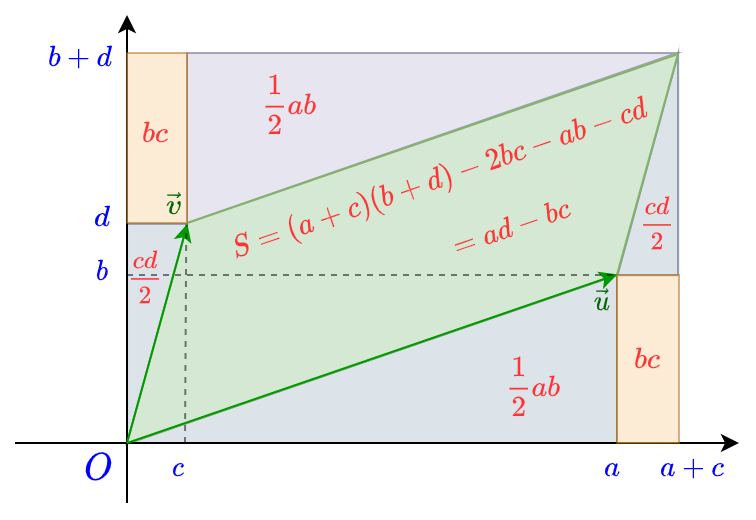
\includegraphics[scale=0.4]{paralel.png}
\end{center}

Теперь введем следующие переобозначения, чтобы связать площадь параллелогорамма с нашей основной темой главы. Положим
$$
\vec u = \vec u^{(1)} = (u^{(1)}_1,u^{(1)}_2), \quad \vec v = \vec u^{(2)} = (u^{(2)}_1,u^{(2)}_2).
$$

Тогда площадь $S$ параллелограмма вычисляется по формуле:
$$
S=\left|u^{(1)}_1u^{(2)}_2-u^{(1)}_2u^{(2)}_1\right|.
$$

\item Мы специально дали номера и векторам, и координатам, чтобы заметить одну особенность: первое произведение в этой формуле выбирает у первого вектора первую координату, а у второго вектора --- вторую. Во втором произведении номера векторов и координат перемешаны. Кроме того, данное выражение, если его взять без модуля, представляет собой определитель матрицы $2\times 2$. Определители матриц используются везде, где работает линейная алгебра --- от решения систем линейных уравнений и искусственного интеллекта до статистики и квантовой механики. В терминах определителя нахождение площди выглядит так:
\begin{center}
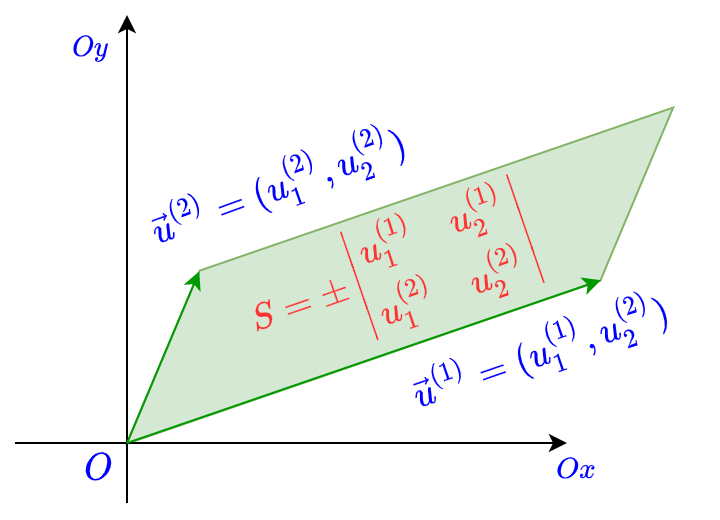
\includegraphics[scale=0.4]{paralel2.png}
\end{center}
Знак $\pm$ означает, что выбирается положительное итоговое значение, т.к. площадь не может быть отрицательной.
\item Но вернемся к перестановкам. Пусть номера векторов --- это элементы множества, на котором выполняется перестановка, а номера координат, выбранных у этих векторов, --- это перестановка номеров векторов. Тогда произведение $u^{(1)}_1u^{(2)}_2$ можно соотнести с тождественной перестановкой $\id=(1)(2)$, а произведение $u^{(1)}_2u^{(2)}_1$ --- с инверсной перестановкой $(12)$. Заметим также, что в случае переставленных номеров перед произведением появляется минус. В то же время, перестановка (12) является нечетной и ее знак тоже равен -1.
\item Аналогичным способом вычисляется объем $V$ параллелепипеда, построенного на трех векторах. Пусть даны три вектора в порстранстве:
$$
u^{(1)}=(u^{(1)}_1,u^{(1)}_2,u^{(1)}_3),\quad u^{(2)}=(u^{(2)}_1,u^{(2)}_2,u^{(2)}_3),\quad u^{(3)}=(u^{(3)}_1,u^{(3)}_2,u^{(3)}_3).
$$
Тогда объем $V$ равен модулю определителя координат трех векторов
$$
V=\pm\begin{vmatrix}
u^{(1)}_1 & u^{(1)}_2 & u^{(1)}_3 \\
u^{(2)}_1 & u^{(2)}_2 & u^{(2)}_3 \\
u^{(3)}_1 & u^{(3)}_2 & u^{(3)}_3 
\end{vmatrix},
$$
а определитель, в свою очередь, вычисляется следующим образом:
\begin{align*}
&
\begin{vmatrix}
u^{(1)}_1 & u^{(1)}_2 & u^{(1)}_3 \\
u^{(2)}_1 & u^{(2)}_2 & u^{(2)}_3 \\
u^{(3)}_1 & u^{(3)}_2 & u^{(3)}_3 
\end{vmatrix} = \sum_{\si\in\Sb_3} \sgn(\si) u^{(1)}_{\si(1)} u^{(2)}_{\si(2)} u^{(1)}_{\si(3)}= \\
& u^{(1)}_1 u^{(2)}_2 u^{(3)}_3 + u^{(1)}_2 u^{(2)}_3 u^{(3)}_1 +
u^{(1)}_3 u^{(2)}_1  u^{(3)}_2 - u^{(1)}_1 u^{(2)}_3  u^{(3)}_2 
 -u^{(1)}_3 u^{(2)}_2  u^{(3)}_1 -u^{(1)}_2 u^{(2)}_1 u^{(3)}_3,
\end{align*}
т.е. мы складываем трехкомпонентные произведения координат от каждого из векторов, используя все перестановки номеров и выставляя знак соответствующей перестановки.

Следующая графическая схема помогает запомнить правило вычисления определителя третьего порядка:
\begin{center}
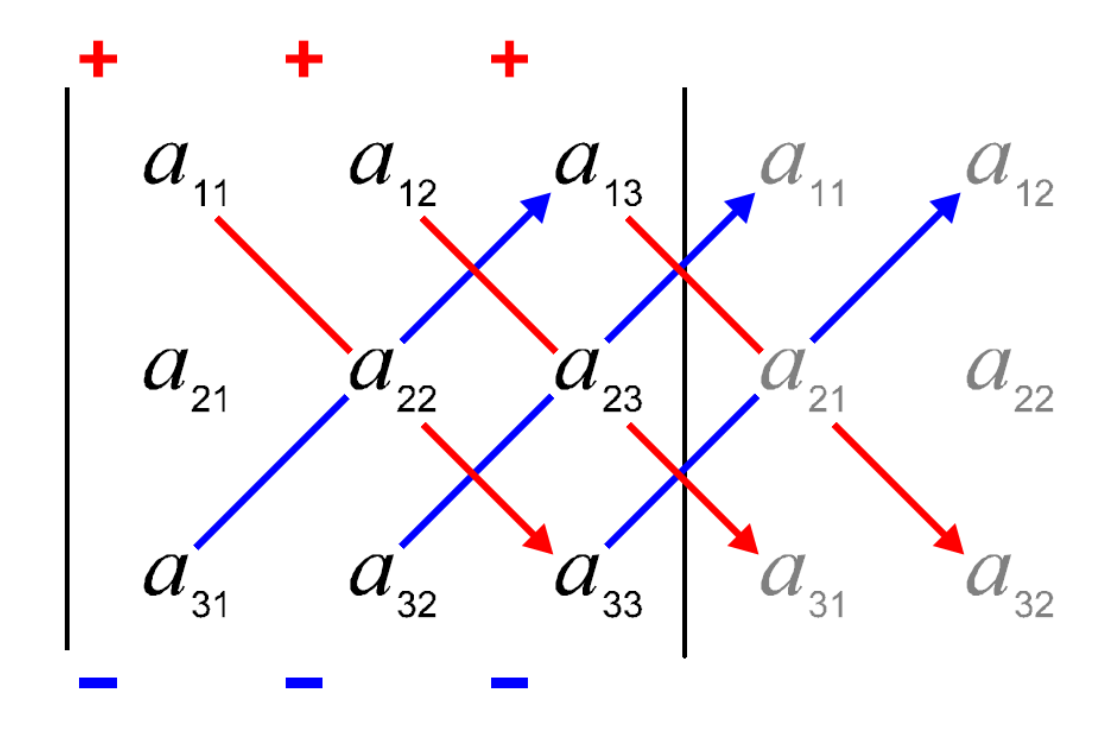
\includegraphics[scale=0.15]{Det.png}
\end{center}

\item На самом деле, и все определители более высокого порядка, и многомерные объемы вычисляются аналогичным способом.

\end{enumerate}



\newchapter[и пространства]{Движения плоскости}

\vrezka{Данная глава продолжает тему групп движений. Здесь мы получаем теорему Шаля (для движений плоскости), а затем широкими мазками освещаем тему движений сферы и пространства. 

Разделы о сфере и пространстве могут быть пропущены при первом ознакомлении с текстом.
}

\section{Виды движений плоскости. Теорема Шаля}

\lesson{Байка про парад. Три вида движения плоскости. Связь с движениями окружности в случае неподвижной точки. Теоремы о неподвижных точках --- двух и трех}

\begin{enumerate}
\item \textbf{Иллюстративная сказка}. Представим себе Красную площадь и парад 9 мая. По площади идут ровные коробки участников парада. Чтобы не нарушать красоту и геометрию движения коробок, солдаты маршируют так, чтобы в каждый момент времени между любыми двумя из них сохранялось одно и то же расстояние. Иначе говоря, они осуществляют движение прямоугольной фигуры по плоскости площади. Затем точно так же делают колонны боевой техники.\index{Движения!плоскости}

По площади все они движутся равномерно и прямолинейно, пока им не придется осуществить поворот сначала на лобном месте на Васильевский спуск, а затем и на Кремлевскую набережную. И всякий поворот ради сохранения стройности шеренг и колонн нужно также осуществлять с сохраненим расстояний между всеми участниками парада. Таким образом движение плоскости можно иллюстрировать прямолинейным смещением и поворотом, а также их последовательными комбинациями.

Наконец, как и в случае окружности, возможно перестроение, при котором внутри одной коробки шеренги меняются ролями: первая шеренга становится последней, вторая --- предпоследней, и так далее. Здесь мы можем вспомнить аналогичную картинку с парковкой автомобилей, которую мы рассматривали ранее при описании движений прямой. Только вместо одного ряда машиномест у нас несколько шеренг. при перестроении они проходят в противоположных направлениях на равные расстояния относительно центральной шеренги. В итоге получается такая ж коробка, только стоявшие впереди участники оказываются сзади, и наоборот. И тут мы снова наблюдаем явление, при котором путаются направления --- вперед и назад. А если бы точно так же переместились колонны внутри коробки, то перепутались бы стороны --- правая и левая. Такое движение, переводящее коробку в себя и меняющее право-лево, либо перед-зад, называется осевой симметрией и оно также, как и в случае окружности, меняет пространственную ориентацию коробки.

\item Вернемся к геометрии.
Из приведенной иллюстрации понятно, что на плоскости существует как минимум три вида движений: параллельный перенос на некоторый вектор $v$, поворот на некоторый угол $\al$ относительно центра вращения в некоторо точке $O$ и симметрия относительно некоторой оси $l$. Первое мы обозначим $T_v$, второе --- $R^O_\al$, третье --- $S_l$. Параллельный перенос на вектор $v$ --- это такое движение, при котором все точки смещаются на вектор $v$ (т.е. в одном и том же направлении на одно и то же расстояние). Поворот --- это такое движение, при котором все точки сдвигаются по концентрическим окружностям на один и тот же угол в одном и том же направлении. Симметрия относительно оси $l$ --- это такое движение, при котором все точки плоскости переходят в симметричные относительно данной оси (т.е. из точки на ось $l$ опускается перпендикуляр, который затем продолжается на такое же расстояние, а все точки $l$ при этом остаются на месте).

\item Для движений плоскости, являющихся параллельным переносом, действует правило сложения параллелограмма. А именно, 
$$
T_v\circ T_u = T_{v+u},
$$
где сумма векторов $v+u$ осуществляется по правилу параллелограмма. Из этого же правила следует, что композиция параллельных переносов есть параллельный перенос, причем порядок слагаемых не имеет значения, т.е. параллельные переносы коммутируют друг с другом.

Для вращений существует аналогичное правило. если они имеют общий центр вращения:
$$
R^O_\al\circ R^O_\be = R^O_{\al+\be}.
$$
Ясно также, что в данном случае вращения коммутируют. т.к. они просто повторяют движения окружности с центром $O$.

Заметим также, что и параллельный перенос, и вращение, и осевая симметрия имеют обратные преобразования. Точнее, $T_v\circ T_{-v}=\id$, $R^O_\al\circ R^O_{-\al}=\id$, а также $S_l\circ S_l=\id$. То есть, эти движения обратимы. Отсюда же следует, что они являются биекциями.

Для вывода остальных свойств арифметики движений нам потребуются некоторые дополнительные сведения о движениях плоскости.

\item Для начала мы рассмотрим случай, когда движение плоскости сохраняет на месте хотя бы одну точку. Назовем такое движение буквой $G$. Выберем какую-нибудь неподвижную точку  движения $G$ и обозначим ее за $O$. Теперь возьмем любую окружность с центром $O$  обозначим ее $S^1$. Что происходит с ней при таком движении? Ясно, что она переходит в себя, поскольку движение сохраняет расстояние, а все точки окружности равноудалеын от центра $O$.

Но тогда получается, что движение $G$ порождает движение окружности $S^1$. Покажем, что разные движения плоскости порождают разные движения окружности. Пусть движения плоскости $G_1$ и $G_2$ оставляют на месте точку $O$, но при этом не равны, т.е. как минимум одна точка $A$ на плоскости переходит в первом случае в $A_1$, а во втором --- в $A_2$, причем $A_1\ne A_2$.

Здесь мы обратимся к одному из важнейших методов геометрии: \textit{проецированию}. А конкретно, --- к проецированию точки на окружность. Соединим точку $O$ с точкой $A$ и, в случае необходимости, продолжим отрезок до пересечения его с окружностью $S^1$ так, чтобы точки $A$ и $A'$ (точка пересечения) лежали по одну сторону от центра $O$. Аналогично построим точки $A_1'$ и $A_2'$.

Далее заметим, что если бы $A_1'=A_2'$, то, очевидно, $A_1$ и $A_2$ оказались бы на одной прямой, причем по одну сторону от $O$. Но в силу свойств движения, т.е. равенства расстояний $|OA_1|=|OA|=|OA_2|$, оказалось бы также, что $A_1=A_2$, что противоречит предположению.

Итак, разные движения плоскости, сохраняющие точку $O$, порождают и разные движения окружности $S^1$ с центром $O$.

Обратно, всякому движению окружности соответствует движение плоскости. Действительно, как мы знаем, движение окружности есть либо вращение, либо симметрия относительно оси, проходящей через центр $O$. В таком случае, возьмем в качестве движения $G$ плоскости либо вращение относительно центра $O$ на тот же угол, либо симметрию относительно той же оси.

Сказанное выше означает, что \textit{все движения плоскости, имеющие общую неподвижную точку $O$, взаимно однозначно определяются одноименными движениями окружности с центром в той же точке $O$}. Говоря алгебраическим языком, множество движений плоскости содержит в себе группы, изоморфные группе движений окружности. Этих групп столько, сколько точек на плоскости.

Чтобы доказать, что все движения плоскости образуют группу, нам потребуется описать все виды движений и построить их таблицу умножения.

\item Редуцирование движений плоскости с неподвижной точкой к движениям окружности, сразу же дает нам возможность понять, что такие движения бывают всего двух видов: повороты (в том числе $\id$) и осевые симметрии. Причем, первый случай получается тогда, когда у движения есть ровно одна неподвижная точка, либо вся плоскость неподвижна. А симмметрия окружности предполагает неподвижность двух диаметриально противоположных точек. Ясно, что при этом не только эти две точки $S^1$ останутся неподвижными.
\begin{lem} Если движение плоскости сохраняет неподвижными две различные точки, то оно сохраняет неподвижными все точки прямой, проходящей через данные две точки.
\end{lem}
\pf Пусть движение $G$ плоскости оставляет на месте точки $A\ne B$. Для начала заметим, что движение $G$ в этом случае прямую $AB$ переводит в саму себя. Действительно, если бы это было не так, то три различные точки $A,B,C$, лежащие на этой прямой, перешли бы в треугольник $ABC'$, где $C'=G(C)$. Но тогда нарушается неравенство треугольника, при котором сумма двух сторон всегда больше третьей, а для трех точек на одной прямой это не так.

Следовательно, $G$ порождает движение прямой $AB$. Но для движения прямой нам уже хорошо известно, что если движение сохраняет на месте две точки на месте, то оно сохраняет все точки этой прямой на месте!
\epf

\item Наконец, остается тривиальный вариант для случая неподвижных точек у движения плоскости.
\begin{thrm}\index{Теорема!о трех гвоздях}
Если движение $G$ плоскости оставляет на месте три точки, не лежащие на одной прямой, то $G=\id$.
\end{thrm}
\pf
Пусть даны три точки $A,B,C$, не лежащие на одной прямой, такие, что $G(A)=A$, $G(B)=B$ и $G(C)=C$. Возьмем окружность $S^1$ с центром в точке $A$. Движение $G$ порождает на этой окружности либо поворот, либо симметрию. Построим проекции точек $B$ и $C$ на данную окружность, получим точки $B'$ и $C'$.

Из доказанной выше леммы следует, что движение $G$ сохраняет на месте прямые $AB$ и $AC$. Эти прямые различны, т.к. иначе бы точки $ABC$ оказались на одной прямой. Следовательно, $A'\ne B'$. В то же время, это точки прямых $AB$ и $AC$, а значит, они являются стационарными точками движения $G$. 

Итак, мы имеем движение окружности, которое сохраняет на месте две различные точки, не являющиеся диаметрально противоположными. А про такое движение мы уже знаем, что является $\id$, т.е. поворотом на нулевой угол. Стало быть, таковым же является и $G$.
\epf

\item Движение плоскости различные точки переводит в различные. Действительно, если бы это было не так, и мы бы имели $G(A)=G(B)$, хотя $A\ne B$, то, взяв произвольную точку $C$, отличную от $A$ и $B$, мы бы получили, что движение $G$ переводит треугольник в отрезок $G(A)G(C)$, что приводит к нарушению неравенства треугольника. Итак, движение плоскости является инъекцией.


\lesson{Движения плоскости: Нет неподвижных точек. Композиция не более трех симметрий. Скользящая симметрия. Теорема Шаля}

\item Посмотрим, что происходит, когда у движения $G$ нет неподвижных точек. Возьмем произвольную точку $O$ и обозначим $A=G(O)$. По предположению $A\ne O$. В таком случае, мы можем построить серединный перпендикуляр отрезка $AO$, который мы обозначим за $l$, и рассмотреть симметрию $S_l$ плоскости относительно него. Тогда, очевидно, композиция движений $S_l\circ G$ сохраняет на месте точку $O$, и мы оказываемся в описанных выше условиях.

Это значит, что движение $S_l\circ G$ является либо поворотом $R^O_\al$ с центром в точке $O$ на угол $\al$, либо симметрией $S_m$ относительно прямой $m$, проходящей через точку $O$. Но тогда, применяя слева симметрию $S_l$, находим, что
$$
G=S_l\circ R^O_\al,\mbox{ либо }G=S_l\circ S_m.
$$

В свою очередь, поворот $R^O_\al$, если его рассматривать как движение окружности $S^1$ с центром $O$, как мы ранее выяснили, является композицией двух симметрий относительно осей $n,k$, угол между которыми равен $\al/2$. Таким образом,
$$
G=S_l\circ S_n\circ S_k,\mbox{ либо }G=S_l\circ S_m.
$$

\item Итак, в том случае, когда движение не сохраняет на месте ни одной точки, оно является композицией двух или трех симметрий.
\begin{thrm}
Всякое движение плоскости есть композиция не более чем трех осевых симметрий.
\end{thrm}
\item Отсюда, в частности, следует, что всякое движение плоскости биективно.

\item Выше мы дали обозначения трем видам движений плоскости: параллельный перенос, поворот и осевая симметрия. Возникает вопрос: исчерпываются ли движения плоскости только такими движениями или есть какие-то еще?

\item Пусть снова движение $G$ таково, что оно не сохраняет на месте ни одной точки. Возьмем произвольную точку $A$ и далее обозначим $B=G(A)$, $C=G(B)$. Поскольку $G$ --- движение (изометрия), $AB=BC$. Если $C$ лежит на прямой $AB$, то вся прямая $A$ под действием движения $G$ пеереходит в себя (иначе бы нарушалось неравенство треугольника), причем точки располагаются в порядке $A<B<C$ (иначе бы мы получили $A=C$, и тогда середина отрезка $AB$ будет стационарной точкой $G$).

Предположим далее, что $C$ не лежит на прямой $AB$. В этом случае обозначим за $X$ середину $AB$, за $Y$ --- середину $BC$, и через точки $X,Y$ проведем прямую $L$. Необходимо показать, что $L$ переходит в себя под действием $G$.

\begin{center}
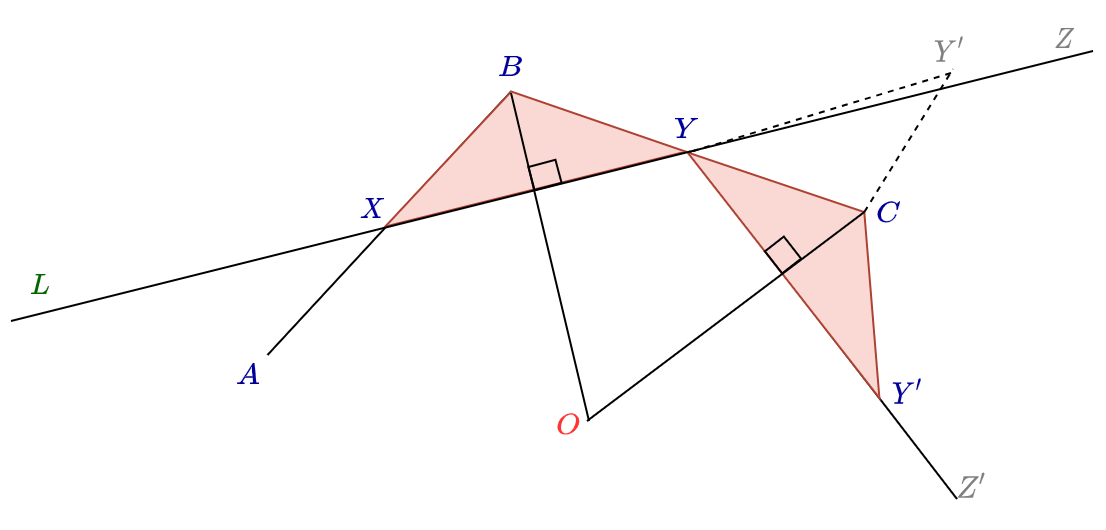
\includegraphics[scale=0.3]{Skolz.png}
\end{center}


Пусть $Y'=G(Y)$. Ясно, что $XY=YY'$, причем $X\ne Y'$, иначе бы середина $XY$ оказалсь стационарной точкой $G$. Точки $X$ и $Y'$ могут лежать по одну или по разные стороны прямой $BC$. Если они лежат по разные стороны, от рассмотрим треугольники $\triangle XYB$ и $\triangle YY'C$. Они равны по трем сторонам в силу того, что $G$ является движением, кроме того, они оба равнобедренные с основаниями $XY$ и $YY'$, соответственно. Но тогда равны углы $\angle XYB=\angle Y'YC$ при вершине $Y$, отложенные в разные стороны прямой $BC$, т.е. эти углы являются вертикальными, откуда следует, что точка $Y'$ находится на прямой $L$. Мы снова получаем ситуацию трех точек в порядке $X<Y<Y'$, откуда следует, что вся прямая $L$ переходит в себя под действием $G$.

Наконец, предположим, что $X$ и $Y'$ оказались по одну сторону прямой $BC$. В этом случае мы можем построить серединные перпендикуляры отрезков $XY$ и $YY'$, которые пересекутся в некторой точке $O$. Пусть $O'=G(O)$. Треугольник $XOY$ равнобедренный, он переходит под действием $G$ в треугольник $YO'Y'$, также равнобедренный. Это значит, что точка $O'$ лежит на серединном перпендикуляре отрезка $YY'$, причем на таком же расстоянии от середины $YY'$, как и точка $O$ от середины  $XY$. Но отрезок $BO$ пересекает отрезок $XY$. Значит, в силу свойств движения, отрезок $CO$ пересекает отрезок $YY'$. И тогда для точки $O'$ остается единственная возможность: $O=O'$. А это противоречит тому, что $G$ не имеет стационарных точек.

Итак, предположение о том, что $G$ не имеет неподвижных точек, приводит к тому, что найдется прямая $L$, которая под действием $G$ переходит в себя. Это значит, что $G$ действует на $L$ как смещение (отражение имело бы неподвижную точку, а других движений на прямой не существует).

Смещение на $L$ задается вектором $XY$ (или $AB$, если мы остались в первом варианте). Составим композицию $G\circ T_{-XY}$. Очевидно, что такое движение плоскости оставляет на месте прямую $L$. Как мы уже выяснили, это соответствует либо $\id$, либо осевой симметрии $S_L$. Таким образом, $G=T_{XY}$, либо $G=S_L\circ T_{XY}$, причем вектор $XY$ параллелен прямой $L$.

\item Итак, движение $G$, которое не сохраняет на месте ни одной точки, является либо параллельным переносом, либо симметрией с последующим параллельным переносом вдоль оси симметрии на ненулевой вектор. Во втором случае движение $G$ называется \textbf{скользящей симметрией}.

\item Легко понять, что скользящая симметрия не сводится к другим видам движений, если ее смещение не нулевое. Действительно, $\id$, поворот и осевая симметрия исключаются из-за наличия неподвижных точек. Параллельный перенос исключается, поскольку при нем отрезок $AG(A)$ не может пересекать никакую прямую, параллельную сдвигу.

\item Скользящую симметрию с осью симметрии $l$ и параллельным переносом вдоль этой оси на вектор $u$ будем обозначать $T_uS_l$ (без значка композиции). Для ее обозначения часто используют символ $W_u$, не указывая явно ось симметрии, т.к. вектор $u$ однозначно ее задает. Но в случае $u=0$ это не так, и поэтому для надежности мы будем использовать два индекса, понимая, что вектор $u$ параллелен оси $l$.

\item Окончательно получаем
\begin{thrm}[Шаля] Всякое движение плоскости (без разложения его на компоненты) есть движение одного из следующих классов:\index{Теорема!Шаля}
\begin{enumerate}[a)]
\item класс параллельных переносов (на произвольный вектор, в том числе нулевой), который мы обозначим $\rightrightarrows$;
\item класс поворотов относительно произвольного центра, который мы обозначим $\circlearrowleft$;
\item класс \textbf{скользящих симметрий} (осевая симметрия с последующим сдвигом на произвольный вектор, параллельный оси симметрии), который мы обозначим $\leftharpoonup\leftharpoondown$.
\end{enumerate}
\end{thrm}
Обычную симметрию относительно неподвижной оси мы теперь отнесем также в класс скользящих симметрий как частный случай при нулевом сдвиге. Точно так же, как относим $\id$ к классу параллельных переносов и поворотов.


\lesson{Построение полной таблицы композиций движений плоскости: переносы и повороты}

\item Таблица композиций для таких классов выглядит следующим образом:\index{Таблица композиций}
\begin{center}
\begin{tabular}{c|ccc}
 & $\rightrightarrows$ & $\circlearrowleft$ &  $\leftharpoonup\leftharpoondown$ \\ \hline
$\rightrightarrows$ & $\rightrightarrows$ &  $\circlearrowleft$ &  $\leftharpoonup\leftharpoondown$  \\ 
$\circlearrowleft$ & $\circlearrowleft$ & $\rightrightarrows$ или $\circlearrowleft$ & $\leftharpoonup\leftharpoondown$  \\ 
$\leftharpoonup\leftharpoondown$ & $\leftharpoonup\leftharpoondown$ & $\leftharpoonup\leftharpoondown$ & $\rightrightarrows$ или $\circlearrowleft$  \\ 
\end{tabular}
\end{center}

Наша дальнейшая задача --- обосновать данную таблицу, построив полную таблицу композиций движений плоскости.

\item Итак, нам нужно найти все попарные комбинации композиций переноса, поворота и скользящей симметрии, причем мы выделим отдельно частный ее случай --- симметрию.

\item Ясно, что $T_u\circ T_v=T_{u+v}$, причем данная композиция коммутативна.

\item Рассмотрим композицию $T_v\circ R_\al^O$. Из свойств движений окружности мы знаем, что поворот можно представить как композицию двух симметрий , а из свойств движений прямой --- что сдвиг тоже можно представить как композицию двух симметрий. Пусть $R_\al^O=S_2\circ S_1$ и $T_v=S_4\circ S_3$. При этом оси симметрий $1$ и $2$ пересекаются в точке $O$, а угол между ними равен $\al/2$ и откладывается от оси 1 к оси 2. Оси 3 и 4 параллельны друг другу и перпендикулярны направлению сдвига, причем расстояние между ними равно $v/2$, а направление сдвига --- от оси 3 к оси 4.

Заметим, что выбор осей 1 и 2 произволен в рамках требований общей точки пересечени и угла между осями. Сама пара осей может быть повернута как угодно, в частности, можно выбрать ось 2 так, чтобы она оказалась перпендикулярной вектору сдвига $v$. Кроме того, выбор осей 3 и 4 также произволен в рамках требований расстояния между ними и строго перпендикулярного положения к вектору сдвига. Саму пару осей можно двигать вдоль вектора $v$ как угодно. Поэтому совместим ось 3 с осью 2.

Имеем следующее:
$$
T_v\circ R_\al^O = (S_4\circ S_3)\circ (S_2\circ S_1) = S_4\circ (S_3\circ S_2)\circ S_1 = S_4\circ S_1,
$$
где мы сократили $S_3\circ S_2$, т.к. это одна и та же симметрия. Полученная композиция $S_4\circ S_1$ является поворотом на тот же угол $\al$, только с новым центром $O_1$, который получем как пересечение осей 1 и 4.
\begin{center}
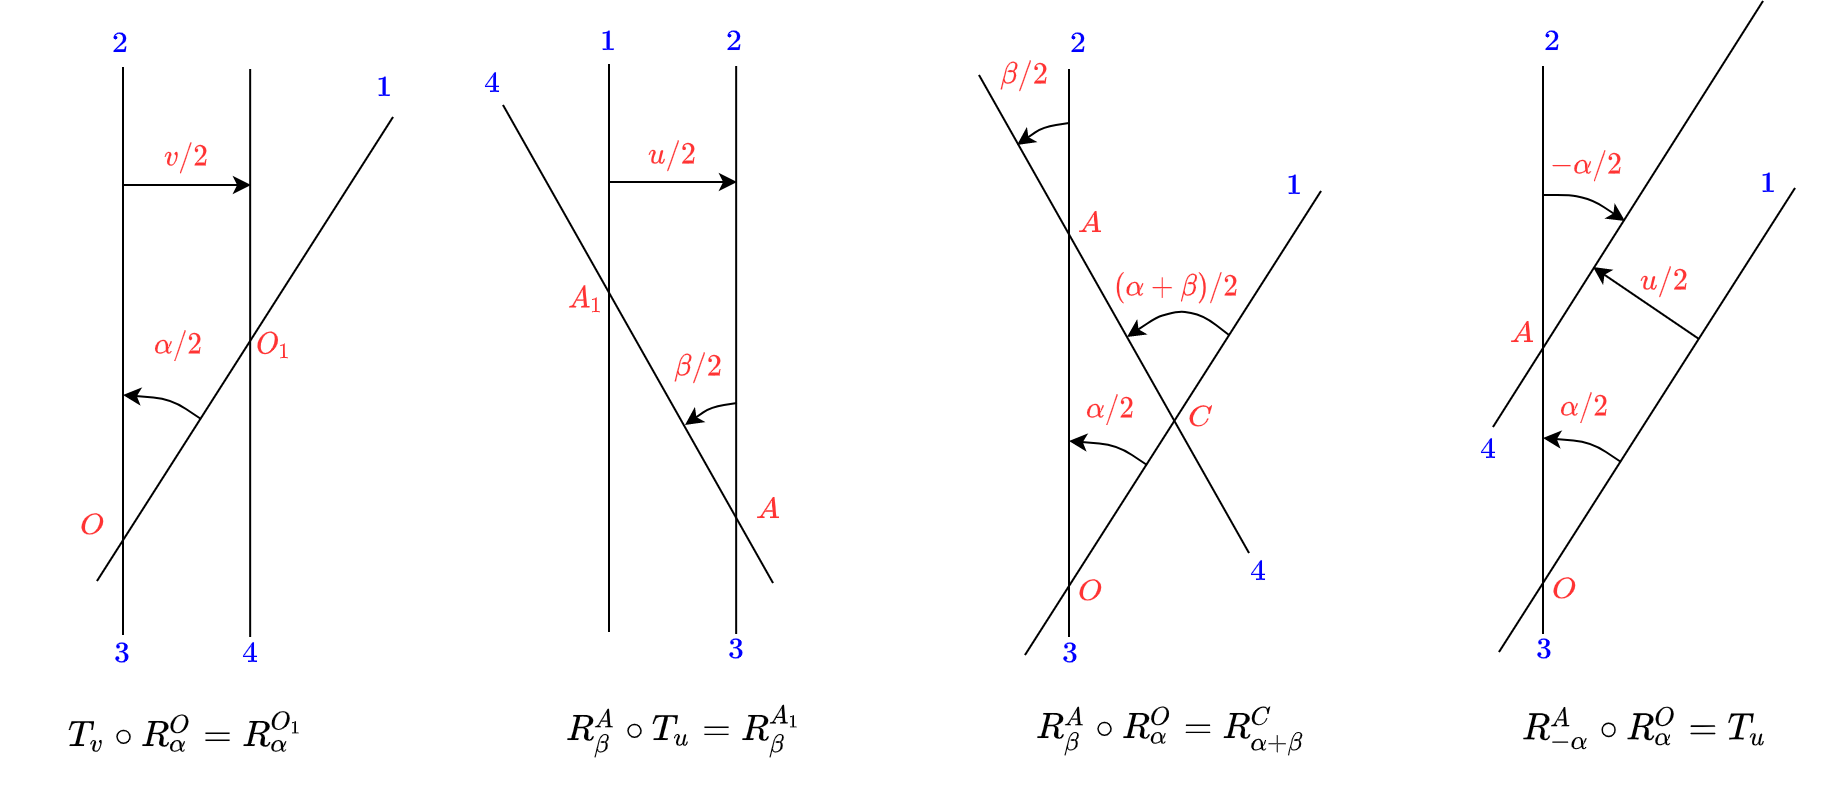
\includegraphics[scale=0.2]{plane_transit.png}
\end{center}

Аналогично поступаем в случае композиции $R_\be^A\circ T_u$ (см. рисунок). При этом новый центр поворота смещается на вектор $-u/2$ и перпендикулярно ему на величину $|u/2|/\tan(\be/2)$. Видим также, что композиция сдвига и поворота не коммутативна (кроме случая, когда перенос осуществляется на нулевой вектор).

\item Рассмотрим композицию двух поворотов $R_\be^A\circ R_\al^O$. Снова представим кажджый поворот как композицию симметрий, и снова, пользуясь произвольностью наклона пары осей симметрий, расположим их так, чтобы вторая ось первого поворота и первая ось второго поворота совпали с прямой $OA$ (см. рисунок). Если углы таковы, что их сумма не равна нулю, то 1 и 4 оси пересекутся, и точка $C$ их пересечения окажется центром результирующего поворота. А угол поворота станет равным $\al+\be$.

Если же $\al+\be=0$, то оси 1 и 4 будут параллельны, и композиция поворотов превратится в паралельный перенос на расстояние $2AO\sin(\al/2)$.

Заметим также, что два поворота будут коммутировать тогда и только тогда, когда $\al=\be$, т.к. только в этом случае точка $C$ будет одна и та же при различном порядке композиции.


\lesson{Таблица композиций движений плоскости: отражения и скользящая симметрия}

\item Рассмотрим композицию $G=T_{\vec v}\circ S_l$. Чтобы понять, что это такое, воспользуемся тем же приемом, с помощью которого мы показали наличие еще одного вида движений плоскости --- скользящей симметрии. Именно, возьмем на прямой $l$ точку $A$ и проследим за ее судьбой при двух итерациях преобразования $G$. Получатся точки $B$ и $C$. Далее, через точки $X$ и $Y$, являющиеся серединами отрезков $AB$ и $BC$, проведем прямую $m$. Эта прямая при преобразовании $G$ переходит сама в себя. Все остальные точки сначала отражаются относительно $m$, затем смещаются в направлении вектора $\vec{AC}$, но на половину его длины. Обозначим $\vec w=\vec{AB}$. Тогда получим, что $G=T_{\vec w}\circ S_m$.

\begin{center}
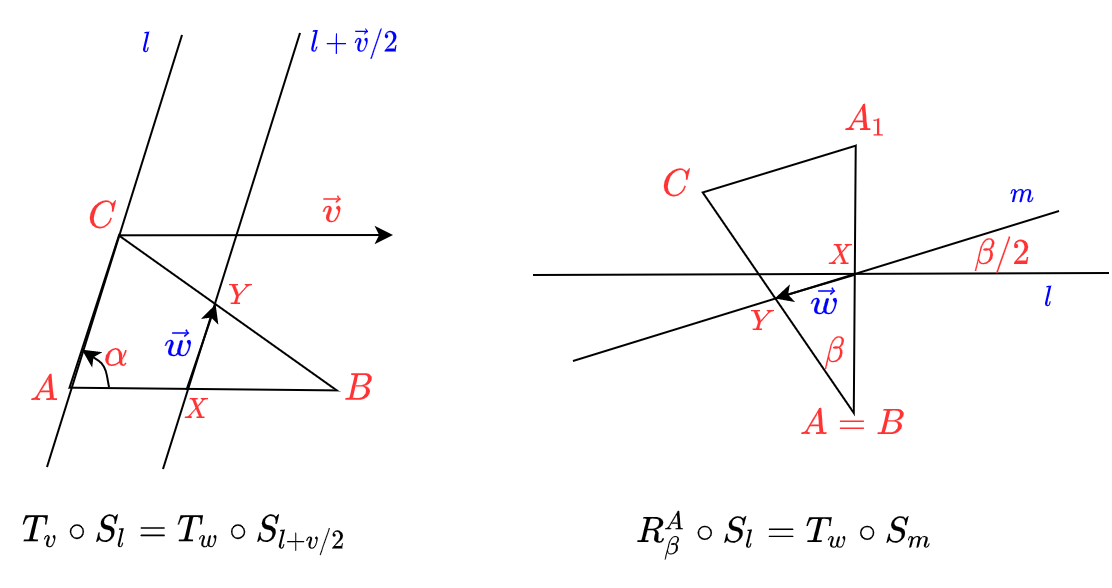
\includegraphics[scale=0.3]{slides.png}
\end{center}

Условимся записывать $\vec w=\Pr_l\vec v$, что означает проекцию вектора $\vec v$ на ось $l$, а также $m=l+\vec v/2$, что означает сдвиг оси $l$ в направлении $\vec v$ на половину его длины. Тогда получим, что
$$
T_{\vec v}\circ S_l = T_{\Pr_l\vec v}\circ S_{l+\vec v/2},
$$
а это не что иное, как скользящая симметрия.

В симметричном случае получим
$$
S_l\circ T_{\vec u} = T_{\Pr_l\vec u}\circ S_{l-\vec u/2},
$$
т.е. тоже скользащая симметрия с тем же сдвигом, но с симметричной относительно $l$ осью симметрии.

Все сказанное справедливо, если угол наклона $l$ не прямой и не нулевой относительно вектора $\vec v$. Если окажется, что $l\perp\vec v$, то $G=S_{l+\vec v/2}$, поскольку смещение $\Pr_l\vec v=0$. Если же $l\parallel\vec v$, то исходное преобразование $G$ уже есть скользаящая симметрия с осью $l$ и смещением $\vec v$. Эти случаи вписываются в общую формулу, если иметь ввиду, что $l+\vec v/2=l$ в том случае, когда $l\parallel\vec v$.

\item Рассмотрим композицию $G=R_\be^A\circ S_l$. В качестве отправной точки $A_1$ возьмем точку, симметричную центру вращения $A$ относительно $l$. Тогда $A_1$ переходит в $A=B$, а далее $B$ переходит в $C$ (см. рисунок). Снова проводим среднюю линию $XY$ в полученном равнобедренном треугольнике. Тогда вектор $\vec w = \vec{XY}$ есть смещение новой скользящей симметрии, а ось $m$, полученная вращением оси $l$ вокруг точки $X$ на угол $\be/2$ --- осью скользящей симметрии.
$$
R_\be^A\circ S_l = T_{\vec w}\circ S_m,\quad \vec w  = 2 \Pr_m\vec{XA},\quad X = \Pr_lA.
$$
Заметим, что в том случае, когда $A\in l$, получаем $\vec w=0$, и композиция $G$ становится просто симметрией $S_m$.

В симметричном случае получим
$$
S_m\circ R_\al^O = T_{-\vec w}\circ S_k,\quad \vec w  = 2 \Pr_k\vec{XO},\quad X = \Pr_mO.
$$

Для внесения данных в итоговую таблицу обозначим за $l+\be/2$ ось $m$, полученную из оси $l$ поворотом на угол $\be/2$ относительно точки $X$ --- проекции центра вращения $A$ на ось $l$. Аналогично, $m-\al/2$. Тогда
$$
R_\be^A\circ S_l = T_w\circ S_{l+\be/2},\quad S_m\circ R_\al^O = T_{-w}\circ S_{m-\al/2}.
$$

\item Композиция двух симметрий $S_m\circ S_l$, как и в случае окружности, есть поворот $R_{2\angle lm}^{l\cap m}$, где $\angle lm$ есть угол от оси $l$ до оси $m$, а центр вращения есть общая точка этих осей. Если угол между осями равен нулю, и при этом они не совпадают, а просто параллельны друг другу, то, как мы уже знаем, их композиция есть параллельный перенос в направлении от $l$ к $m$ (перпендикулярно им) на удвоенное расстояние между осями симметрии. Такой перенос обозначим $T_{2(m-l)}$.

\item Осталось рассмотреть композиции со скользящей симметрией. Пусть $G=T_v\circ T_uS_l$. Очевидно, что это на самом деле композиция $T_{u+v}\circ S_l$, и мы приходим к уже рассмотренному случаю композиции переноса и симметрии. Обратно, если $G$ есть композиция $T_vS_m\circ T_u$, то поскольку в скользящей симметрии перенос и симметрия коммутируют, запишем $G$ как
$S_m\circ T_{v+u}$, и мы снова имеем дело с изученной ситуацией.

\item Пусть далее $G=R_\be^A\circ T_uS_l$. В таком случае
$$
G = (R_\be^A\circ T_u)\circ S_l = R_\be^{A_1}\circ S_l,
$$
т.е. снова приходим к изветсному случаю с заменой лишь центра вращения. В симметричном случае $T_vS_m\circ R_\al^O$ все аналогично.

\item Наконец, пусть $G=S_m\circ T_uS_l$. Здесь можно пойти разными путями для получения результата. Проще выглядит путь, при котором мы сначала найдем композицию двух симметрий:
$$
G = (S_m\circ S_l)\circ T_u = \begin{cases} R_{2\angle ml}^O, & l\not\parallel m, \\
T_{2(m-l)+u}, & l\parallel m,\end{cases}
$$
в первом случае центр симметрии $O$ зависит от вектора $u$.

Аналогично,
$$
T_vS_m\circ S_l = T_v\circ(S_m\circ S_l) = \begin{cases} R_{2\angle ml}^O, & l\not\parallel m, \\
T_{2(m-l)+v}, & l\parallel m,\end{cases}
$$
где центр симметрии $O$ зависит от вектора $v$.

\item Осталось рассмотреть случай композиции двух скользящих симметрий:
$$
T_vS_m\circ T_uS_l = T_v\circ(S_m\circ S_l)\circ T_u =\begin{cases} R_{2\angle ml}^O, & l\not\parallel m, \\
T_{2(m-l)+u+v}, & l\parallel m,\end{cases}
$$
где центр симметрии $O$ зависит уже от обоих переносов $u$ и $v$.

\item Сведем все полученные результаты в таблицу.\index{Группа!движений плоскости}

\renewcommand{\arraystretch}{1.8}\renewcommand{\tabcolsep}{1mm}
\begin{center}\tiny
\begin{tabular}{c|c|c|c|c|}
$\id$  &  $T_u$      &   $R_\al^O$   &   $S_l$   & $T_uS_l$  \\
\hline
$T_u$  &  $T_{u+v}$  &   $R_\al^{O_1}$ & $T_{\Pr_lv}S_{l+v/2}$ & $T_{\Pr_l[u+v]}S_{l+(u+v)/2}$ \\ \hline 
$R_\be^A$ & $R_\be^{A_1}$ & \specialcell{$R_{\al+\be}^C$ ($\al+\be\ne 0$) \\ $T_w$ ($\al+\be=0$)} & \specialcell{$T_wS_{l+\be/2}$ ($A\notin l$) \\ $S_{l+\be/2}$ ($A\in l$)} & \specialcell{$T_wS_{l+\be/2}$ ($A_1\notin l$) \\ $S_{l+\be/2}$ ($A_1\in l$)} \\ \hline 
$S_m$ & $T_{\Pr_lu}S_{m-u/2} $ & \specialcell{$T_wS_{m-\al/2}$ ($O\notin m$) \\ $S_{m-\al/2}$ ($O\in m$)} &
\specialcell{$R_{2\angle lm}^{l\cap m}$ ($l\not\parallel m$) \\ $T_{2(m-l)}$ ($l\parallel m$)} & 
\specialcell{$R_{2\angle lm}^O$ ($l\not\parallel m$) \\ $T_{2(m-l)+u}$ ($l\parallel m$)} \\ \hline 
$T_vS_m$ & $T_{\Pr_l[u+v]}S_{m-(u+v)/2}$ & \specialcell{$T_wS_{m-\al/2}$ ($O_1\notin m$) \\ $S_{m-\al/2}$ ($O_1\in m$)} &
\specialcell{$R_{2\angle lm}^O$ ($l\not\parallel m$) \\ $T_{2(m-l)+v}$ ($l\parallel m$)} &
\specialcell{$R_{2\angle lm}^O$ ($l\not\parallel m$) \\ $T_{2(m-l)+u+v}$ ($l\parallel m$)} \\ \hline
\end{tabular}
\end{center}

\end{enumerate}


\subsection*{Задачи}
\begin{enumerate}
\item Найти композицию отражения относительно вертикальной оси и поворота на $180^o$ относительно точки, не лежащей на оси симметрии.
\item Пусть дан произвольный треугольник. На его сторонах построим правильные треугольники и соединим их центры. Жоказать, что полученный треуголник --- правильный.
\end{enumerate}


\section{Сравнение движений прямой, окружности и плоскости}


\lesson{Общие слова о схожести движенией прямой и окружности, окружности и плоскости. Понятие ориентации}

\begin{enumerate}
\item Отметим несколько общих свойств рассмотренных нами движений прямой, окружности и плоскости.
\item Во-первых, их всех можно свести к композиции симметрий. Для одномерных объектов (прямая и окружность) --- не более двух, для двумерных --- не более трех.
\item Во-вторых, все движения можно разделить на два класса: сохраняющие и меняющие \textbf{ориентацию}. Те движения, которые сводятся к композиции четного числа симметрий, сохраняют ориентацию фигур, а те, которые сводятся к композиции нечетного числа симметрий, --- меняют ориентацию фигур. Изменение ориентации означает, что право и лево меняются местами, т.е. мы как бы переходим в зазеркалье. 
\item При этом нужно отметить, что преобразования, меняющие ориентацию, обязательно требуют выхода в пространство более высокой размерности (для прямой --- в плоскость, а для окружности и плоскости --- в пространство размерности 3), если мы хотим осуществить их непрерывным движением.
\item В-третьих, есть и более глубинная связь движений прямой, окружности и плоскости. Мы уже отмечали, что окружность можно рассматривать как прямую, у которой склеили противоположные концы (где-то на бесконечности). И с этой точки зрения сдвиг на прямой является прямой аналогией вращения окружности. Особенно, если величина сдвига сильно меньше радиуса.
\item А симметрия прямой при этом естественным образом превращается в симметрию окружности. Только ось симметрии должна проходить через место склейки двух бесконечностей. Остальные же симметрии можно получить дополнительным сдвигом, т.е. вращением.
\item Далее, окружность находится на плоскости. И поэтому вращение окружности полностью аналогично вращению плоскости, если при этом совместить их центры.
\item Еще проще увидеть совпадения понятий сдвига на прямой и плоскости. В обоих случаях мы просто смещаем все точки на какой-то вектор.
\item Тем не менее, на плоскости появляется новый вид движения, который комбинирует в себе сдвиг и отражение относительно оси сдвига. Это --- скользаящая симметрия, т.е. симметрия с последующим применением сдвига вдоль оси симметрии. На одномерных объектах такое движение в принципе невозможно. На прямой симметрия относительно этой же прямой ничего не дает, т.е. является $\id$, а на окружности симметрия относительно самой окружности вообще требует специального построения в геометрии плоскости.
\end{enumerate}



\section{Пара слов о движениях сферы}


\lesson{Движения сферы: вращения, отражения, зеркальные вращения (аналог скользящей симметрии). Теорема Шаля}

\begin{enumerate}\index{Движения!сферы}
\item Имея опыт перехода от прямой к окружности, мы можем легко найти движения сферы, отправляясь от движений плоскости.
\item Представим себе сферу как плоскость, у которой бесконечно удаленный край был стянут в точку (метод <<хинкали>>).
\item Во что превращаются при этом движения плоскости?
\item Сдвиг, он же параллельный перенос, превращается в такое движение, при котором все точки движутся по параллельным траекториям. С точки зрения географии это есть движение вдоль широтных линий. Да, проходят они при этом разное расстояние! Из-за чего, кстати, и появляются силы Кориолиса, создающие океанические течения вроде Гольфстрима. Но собственные расстояния между точками сохраняются, и это, несомненно, движение.
\item Вращение, которое, как мы помним, на окружности соответствует сдвигу на прямой, в случае сферы в прямом смысле слова совпадает со сдвигом! Дело в том, что вращение сферы вокруг оси, --- это вращение вокруг полюса, при котором угол поворота измеряется меридианом. Но ведь то же самое движение около экватора есть то, что мы только что отнесли к сдвигам вдоль широтных линий.
\item Таким образом, сдвиг прямой и вращение окружности в случае сферы чудесным образом объединяются в один вид движений --- осевое вращение. И это делает движения сферы чуть проще, чем движения плоскости, где сдвиг можно представить лишь как композицию двух вращений.
\item Далее, симметрия плоскости относительно прямой естественным образом переходит в отражение сферы относительно центральной секущей плоскости или, иначе говоря, относительно окружности большого круга. При такой симметрии полюса сферы меняются местами (полюса определются пересечением со сферой прямой, пересекающей плоскость отражения в центре сферы и перпендикулярной ей), а плоскость отражения остается на месте.
\item Наконец, скользящая симметрия плоскости есть композиция сдвига и осевой симметрии, и ей на сфере соответствует \textbf{зеркальное вращение}, т.е. композиция отражения и вращения параллельно плоскости отражения.
\item Таким образом, все движения сферы распадаются на два класса: вращения и зеркальные вращения. При этом, все движения есть композиция не более чем трех отражений.
\item Этот аналог теоремы Шаля для сферы можно доказать, используя очередную лемму о гвоздях, предполагая неподвижность пары противоположых точек (случай одной точки на плоскости), неподвижность целой окружности большого круга (случай двух точек на плоскости), отсутствие неподвижных точек.
\end{enumerate}

\subsection*{Задачи}
\begin{enumerate}
\item Построить таблицу движений сферы аналогично таблице движений плоскости (символику придумайте сами).
\item **Доказать, что других движений на сфере не существует (лемма о гвоздях).
\end{enumerate}


\section{Пара слов о движениях пространства}



\lesson{Движения пространства: винт (в частности, сдвиг, осевое вращение, $\id$), зеркальное вращение (в частности, отражение), скользящая симметрия (в частности, отражение). Итоговая таблица классов собственных и несобственных движений прямой, окружности, плоскости, сферы и пространства}

\begin{enumerate}\index{Движения!пространства}
\item Наконец, мы можем от сферы перейти к пространству. На самом деле, переход в пространство сопровождается лишь добавлением сдвига в пространстве. Т.е. любое движение сферы можно рассматривать как движение пространства с одной неподвижной точкой --- центром сферы. После чего можно применить сдвиг этого центра, и получить новые движения. Понятно, что никаких других движений тут быть не может.
\item Тем не менее, классификация движений пространства становится сложнее примерно так же, как классификация движений плоскости превосходит классификацию движений окружности. А именно, в пространстве появляется \textbf{винтовое движение} как композиция осевого вращения и сдвига вдоль оси вращения. Это --- обобщение скользящей симметрии на плоскости (если винт осуществляет поворот на $180^0$, мы как раз получаем скользящую симметрию).
\item Есть также и собственно \textbf{скользящая симметрия пространства}. Это --- отражение относительно плоскости с последующим сдвигом вдоль направления, параллельного данной плоскости. Такое движение также является обобщением скользящей симметрии на плоскости.
\item Заметим, что более сложное движение винт включает в себя более простые. Так, если винт имеет нулевой сдвиг, то он доставляет осевое вращение, а если винт имеет нулевой поворот, то он доставляет сдвиг. Понятно, что в случае полного зануления параметров винта мы получим $\id$.
\item Точно так же, \textbf{зеркальное вращение}, как и в случае сферы, при нулевом повороте доставляет просто симметрию.
\item Наконец, скользящая симметрия своим частным случаем имеет просто симметрию относительно плоскости.
\item Таким образом, классификация движений пространства включает следующие виды движений:
\begin{enumerate}[a)]
\item винт (в частности, сдвиг, осевое вращение, $\id$);
\item зеркальное вращение (в частности, отражение);
\item скользящая симметрия (в частности, отражение).
\end{enumerate}
\end{enumerate}

\subsection*{Задачи}
\begin{enumerate}
\item Построить таблицу движений пространства аналогично таблице движений плоскости (символику придумайте сами).
\item *Показать, что центральная симметрия пространства --- это зеркальное вращение.
\item **Доказать, что других движений в пространстве не существует (лемма о гвоздях).
\end{enumerate}


\begin{sidewaystable}
\caption{Сравнение движений.}
\label{Transitions}
\begin{tabular}{p{2cm}|p{2.5cm}p{2.5cm}p{2.5cm}p{2cm}p{2.5cm}p{2.5cm}}
\rowcolor{darkred}
& \multicolumn{3}{P{8.5cm}}{\textcolor{white}{\bfseries Собственные движения\linebreak (не меняют ориентацию)}} & \multicolumn{3}{P{8cm}}{\textcolor{white}{\bfseries Несобственные движения\linebreak (меняют ориентацию)}} \\ 
& Перенос & Поворот & Смещение поворота & Симметрия & \multicolumn{2}{p{5cm}}{Смещенная симметрия} \\ \hline \hline
Прямая     & сдвиг на число & & & относи\-тель\-но точки & & \\  \hline
Окруж\-ность & \multicolumn{2}{p{5cm}}{\centerline{вращение}} & & осевая симметрия & & \\ \hline
Плос\-кость  & параллель\-ный перенос & относи\-тель\-но точки & & осевая симметрия & скользящая симметрия (перенос+ сим\-мет\-рия) & \\  \hline
Сфера & вращение вблизи экватора & вращение вблизи полюса & & отражение относительно плоскости & \multicolumn{2}{p{5cm}}{зеркальное вращение (вращение+симметрия)} \\ \hline
Прост\-ранство & параллель\-ный перенос & осевое вращение & винт (перенос + вращение) & отражение относительно плоскости & скользящая симметрия (перенос+ сим\-мет\-рия) & зеркальное вращение (вращение+ сим\-мет\-рия) \\ \hline \hline
\end{tabular}
\end{sidewaystable}


